\documentclass{beamer}
\usepackage{amsmath}
\usepackage{amssymb}
\usepackage{graphics}
\usepackage{booktabs}
\usepackage{hyperref}
\usepackage{rotating}
\usepackage{multirow}
\usepackage{eurosym}
\usepackage{colortbl,color}
\usetheme{default}
\renewcommand{\theenumii}{\alph{\enumii}}
\defbeamertemplate{itemize subitem}{dash}{--}
\defbeamertemplate{itemize subsubitem}{dash}{--}
\setbeamertemplate{itemize item}[circle]
\setbeamertemplate{itemize subitem}[dash]
\setbeamertemplate{itemize subsubitem}[dash]
\setbeamertemplate{enumerate item}{\arabic{enumi}.}
\setbeamertemplate{enumerate subitem}{(\alph{enumii})}
\usefoottemplate{}
\newcommand{\RedOverlay}[1]{\only{\color{red}{#1} }}
\newcommand{\bluetext}[1]{{\color{blue}{#1} }}
\newcommand{\redtext}[1]{{\color{red}{#1} }}
\newcommand{\UNCOVER}[3]{\only<#2>{\color{white}{#1}}\only<#3>{#1}}
\newcommand{\UNCOVERR}[4]{\only<#2>{\color{white}{#1}}\only<#3>{\color{red}{#1}}\only<#4>{#1}}
\newcommand{\showOn}[3]{\only<#2>{\color<#2>{black} #1}\only<#3>{\color<#3>{white} #1}}
\setbeamertemplate{headline}{}
\usenavigationsymbolstemplate{}
\setbeamercolor{titlelike}{fg=black}
\setbeamercolor{item}{fg=black}

\newcommand{\indicator}[1]{\mathrm{1}\left\{{#1}\right\}}

\title{\LARGE Econ 2220: Experimental Economics \\ Dynamic Games}
\author{Alistair J. Wilson }
\date{Fall 2018}
\begin{document}
\maketitle


\begin{frame}{Introduction}
	\begin{itemize}
		\item Many interesting one-shot interactions have inefficient Nash outcomes
		\item But observed lab behavior frequently exhibits deviations to efficiency
		\item In longer-run relationships, players who value the future enough can
		obtain efficient outcomes in equilibrium
			\begin{itemize}
				\item Observed behavior indicates an affinity for conditionally cooperative
			responses to achieve efficiency
			\end{itemize}
		\item In environments where the game is also evolving (\textbf{dynamic games}),
		the standard solution concept ignores the most-efficient equilibrium
		strategies
	\end{itemize}
\end{frame}



\begin{frame}{One-Shot Prisoner's Dilemma}
	\begin{center}
		\begin{tabular}{cc|p{0.14\textwidth}|p{0.14\textwidth}|}
		 & \multicolumn{1}{c}{} & \multicolumn{2}{c}{2:}\\
		 & \multicolumn{1}{c}{} & \multicolumn{1}{p{0.14\textwidth}}{\textbf{C}} & \multicolumn{1}{p{0.14\textwidth}}{\textbf{D}}\\
		\cline{3-4}
		\multirow{2}{*}{1:} & \textbf{C} & 100,100 & 30, 125\\
		\cline{3-4}
		 & \textbf{D} & 125, 30 & \textbf{60,60}\\
		\cline{3-4}
		\end{tabular}
	\end{center}

	\begin{itemize}
		\item Unique Nash prediction is joint defection
		\item But the outcome is inefficient
	\end{itemize}
\end{frame}

\begin{frame}{One-Shot Prisoner's Dilemma}
\begin{center}
\begin{tabular}{cc|p{0.14\textwidth}|p{0.14\textwidth}|}
 & \multicolumn{1}{c}{} & \multicolumn{2}{c}{2:}\\
 & \multicolumn{1}{c}{} & \multicolumn{1}{p{0.14\textwidth}}{\textbf{C}} & \multicolumn{1}{p{0.14\textwidth}}{\textbf{D}}\\
\cline{3-4}
\multirow{2}{*}{1:} & \textbf{C} & 100,100 & 30, 125\\
\cline{3-4}
 & \textbf{D} & 125, 30 & \textbf{60,60}\\
\cline{3-4}
\end{tabular}
\end{center}
\begin{itemize}
\item Even when the game is repeated finitely, the unique equilibrium prediction
is joint defection.
\end{itemize}
\end{frame}

\begin{frame}{Prisoner's Dilemma Experiments}
Early experiments in the 1950s on behavior in one-shot PD games (but
with repeated play) led to the following point made my John Nash:
\begin{quotation}
The flaw in the experiment as a test of equilibrium point play is
that the experiment really amounts to having the players play one
large multimove game... In this view, it is still true that the only
real absolute equilibrium point is for {[}1+2 to always play C{]}.
However, the strategies:\end{quotation}
\begin{itemize}
\item {[}1{]} plays {[}C{]} til {[}2{]} plays {[}D{]}, then {[}D{]} ever
after,
\item {[}2{]} plays {[}C{]} til {[}1{]} plays {[}D{]}, then {[}D{]} ever
after,\end{itemize}
	\begin{quotation}
	are very nearly at equilibrium, and in a game with an indeterminate
	stop point or an infinite game with interest on utility, it \textbf{is}
	an equilibrium point.
	\end{quotation}
\end{frame}

\begin{frame}{Indefinitely Repeated Prisoner's Dilemma}
\begin{center}
\begin{tabular}{ccccp{0.14\textwidth}|p{0.14\textwidth}cp{0.4\textwidth}}
 & \multicolumn{3}{c}{\textbf{Game }$\Gamma:$} & \multicolumn{2}{c}{\textbf{Play}} &  & \textbf{Then}\\
 &  &  &  & \multicolumn{2}{c}{2:} &  & \\
 &  &  &  & \multicolumn{1}{p{0.14\textwidth}}{\textbf{C}} & \textbf{D} &  & \\
\cline{5-6}
 &  & \multirow{2}{*}{1:} & \multicolumn{1}{c|}{\textbf{C}} & 100,100 & \multicolumn{1}{p{0.14\textwidth}|}{30, 125} &  & Probability $\delta$, play $\Gamma$\\
\cline{5-6}
 &  &  & \multicolumn{1}{c|}{\textbf{D}} & 125, 30 & \multicolumn{1}{p{0.14\textwidth}|}{60,60} &  & Probability $(1-\delta)$, End\\
\cline{5-6}
\end{tabular}
\par\end{center}
\begin{itemize}
\item Model of an ongoing relationship
\item We can interpret $\delta$ here as

\begin{itemize}
\item the amount we value the future,
\item the present value of future gains $\nicefrac{1}{(1+r)}$
\item likelihood of relationship surviving \pause
\end{itemize}
\item So long as $\delta$ is large enough we get the result Nash alludes
to
\end{itemize}
\end{frame}\begin{frame}{Conditional Cooperation}
\begin{itemize}
\item Take an infinitely repeated Prisoner's Dilemma with Nash's strategy

\begin{itemize}
\item Partner cooperates so long as I have (historically), but, if they
observe a defection, they switch to a punishment
\item If the punishment's costs are larger than the benefits from deviating,
then efficient cooperation can be sustained
\end{itemize}
\end{itemize}
\end{frame}\begin{frame}{Conditional Cooperation}

\begin{center}
\begin{tabular}{cc|p{0.14\textwidth}|p{0.14\textwidth}|}
 & \multicolumn{1}{c}{} & \multicolumn{2}{c}{2:}\\
 & \multicolumn{1}{c}{} & \multicolumn{1}{p{0.14\textwidth}}{\textbf{C}} & \multicolumn{1}{p{0.14\textwidth}}{\textbf{D}}\\
\cline{3-4}
\multirow{2}{*}{1:} & \textbf{C} & 100,100 & 30, 125\\
\cline{3-4}
 & \textbf{D} & 125, 30 & 60,60\\
\cline{3-4}
\end{tabular}
\par\end{center}
\begin{itemize}
\item If both players follow the strategy the expected outcome is:

\begin{itemize}
\item $100+\delta\cdot100+\delta^{2}\cdot100+\ldots\sim(1-\delta)100+\delta\cdot100$\pause
\end{itemize}
\item Consider a deviation to playing $D$, this yields

\begin{itemize}
\item $125+\delta\cdot60+\delta^{2}\cdot60+\ldots\sim(1-\delta)125+\delta\cdot60$\pause
\end{itemize}
\item Gain from deviation of $(1-\delta)\cdot25$, cost of $\delta\cdot40$
\item Equilibrium to conditionally cooperate whenever $\delta\cdot40\geq(1-\delta)\cdot25\rightarrow\delta\geq\nicefrac{5}{13}$
\end{itemize}
\end{frame}\begin{frame}{Folk Theorems}
\begin{itemize}
\item Moreover, if $\delta$ is large enough, we get the folk theorem result
that

\begin{itemize}
\item Any payoff profile for the agents in the game that is above the individually
rational payoff is supportable as a sub-game perfect equilibrium outcome
\end{itemize}
\end{itemize}
(cf. Fudenberg \& Maskin, EMA 1986)

\end{frame}

\begin{frame}{Folk Theorem: Graphical Representation}

\begin{center}
	\includegraphics<1>[width=0.6\textwidth]{../../../../p/vw_MPE/img/col_GamePayoffsLow.pdf}
\end{center}
	\begin{itemize}
		\item Multiplicity of equilibrium outcomes
	\end{itemize}
\end{frame}

\begin{frame}{Experimental Selection}
	\begin{itemize}
	\item Given a multiplicity of outcomes for $\delta$ large enough, an experimental
	literature has examined selection in these environments\pause
	\item Main findings:

		\begin{itemize}
		\item where $\delta$ allows for conditional cooperation to emerge, human
		subjects for the most part select cooperative strategies (Dal B\'o,
		AER 2005)
		\item The riskiness of coordinating on cooperation helps us understand selection
		(Dal B\'o and Fr\'echette, AER 2011)
		\item In extensions to environments with imperfect monitoring we see greater
		forgiveness and leniency in strategy selections (Fudenberg et al,
		AER 2013)
		\end{itemize}
	\end{itemize}
\end{frame}

\begin{frame}{Future payoffs determined by actions today}

\begin{itemize}
\item In infinitely repeated games, the strategic environment each period
is constant
\item In dynamic environments, the game being played evolves through time

\begin{itemize}
\item For instance, Prisoner's Dilemma with changing stakes
\item Classic example: common-pool problems\pause

\begin{itemize}
\item State is the number of fish in the pond
\item In each period, participants choose to take a large or small number
of fish
\item The stock of fish next period depends on the number of fish not taken
today.
\item Efficient outcome to grow the stock, and farm the resource
\end{itemize}
\end{itemize}
\item Dynamic incentives can act through the state transition and other's
actions
\end{itemize}
\end{frame}

\begin{frame}{Dynamic Game}
\begin{itemize}
\item Basic features

\begin{itemize}
\item Players $i\in\mathcal{I}$
\item Periods $0,1,\ldots,t,\ldots$
\item Period action $a_{t}^{i}\in A_{i}$; action profile $a_{t}\in\mathcal{A}=\times_{i\in\mathcal{I}}\mathcal{A}_{i}$\pause
\item State $\omega_{t}\in\Omega$
\item State Transition Rule $\psi:\Omega\times\mathcal{A}\rightarrow\Delta\Omega$,
next period's state $\omega_{t+1}=\psi(\omega_{t},a_{t})$\pause
\item Period payoffs: $\pi_{t}^{i}=u^{i}(a_{t},\omega_{t})$
\item History: $h_{t}=\left((a_{1},\omega_{1}),...,(a_{t-1},\omega_{t-1})\right)$\pause
\end{itemize}
\item Large set of SPE is possible (Folk theorem, Dutta, JET 1995)
\end{itemize}
\end{frame}


\begin{frame}{Dynamic Game}
\begin{itemize}
\item Whereas infinitely repeated games look at \emph{sub-game perfect}
outcomes, dynamic games focus on refinement: \emph{Markov Perfection}

\begin{itemize}
\item a Markov Strategy profile ($\alpha:\Omega\rightarrow\mathcal{A}$)
\item Players actions

\begin{itemize}
\item does not depend on any element of $h_{t}$
\item stationary (no time dependence)
\item reacts only to the contemporaneous state $\omega_{t}$
\end{itemize}
\item For an infinitely repeated PD games this picks $(D,D)$ forever
\end{itemize}
\end{itemize}
\end{frame}\begin{frame}{Markov Strategies (from Maskin \& Tirole, 2001)}

Why the Markov Perfect restriction?
\begin{itemize}
\item Philosophically:

\begin{itemize}
\item ``Simplest form of behavior consistent with rationality''
\item ``Bygones are bygones''
\item ``Minor causes should have minor effects''
\end{itemize}
\item Practically:

\begin{itemize}
\item Easy to solve with dynamic programming tools

\begin{itemize}
\item Reduces multiplicity
\item Allows for econometric estimation of models
\item Markov restriction can in principle be tested
\end{itemize}
\end{itemize}
\end{itemize}
\end{frame} \begin{frame}{Markov Strategies: Practical Uses}

Used as main solution concept in dynamic environments
\begin{itemize}
\item Theory

\begin{itemize}
\item Oligopoly with investment
\item Political economy models with durable public goods
\item Environmental economics
\end{itemize}
\item IO assessments of model parameters estimated using MPE to identify
\end{itemize}
\end{frame}
\begin{frame}{Markov Strategies }

\begin{itemize}
\item Potential issues:

\begin{itemize}
\item Inefficiency (does not necessarily lead to efficient outcomes)
\item Lack of precise evidence for the restriction
\item Policy recommendations can depend on equilibrium selection
\item What exactly is the correct set of states?

\begin{itemize}
\item (for Maskin \& Tirole states must be payoff relevant)
\end{itemize}
\end{itemize}
\item Our aim is to examine the Markov Perfect restriction
\end{itemize}
\end{frame}

\begin{frame}{Battaglini, Nunnari and Palfrey (2014)}
\begin{itemize}
	\item Examine a dynamic public good problem
	\item Round payoff is given by
	$$ u_i(x^j_t,g_t)=x^j_t+\alpha \cdot \sqrt{g_t}$$
	\begin{itemize}
	\item $g_t$ is the stock of the public good
	\item $x^j_t$ is private consumption
	\end{itemize} \pause
	\item Payoff for entire supergame is
	$$ \sum_{t=1}^{\infty} \delta^{t-1} \cdot u_i(x^j_t,g_t) $$
\end{itemize}
\end{frame}

\begin{frame}{Battaglini, Nunnari and Palfrey (2014)}
\begin{itemize}
	\item Initially public good has zero investment $g_0=0$
	\item Each period, the agents receive income of $w$ which they allocate to
	\begin{itemize}
		\item $x^j_t$ private consumption
		\item $w-x^j_t$ contribution to public good
	\end{itemize}\pause
	\item The public good grows according to:
	$$ g_t=g_{t-1}+\sum^n_{j=1} (w-x^j_t)$$
\end{itemize}
\end{frame}

\begin{frame}{Battaglini, Nunnari and Palfrey (2014)}
	\begin{itemize}
		\item Like a standard public goods problem, there is a static externality
		\begin{itemize}
			\item Internalize opportunity cost of contributing to public good
			\item Do not internalize public benefit
		\end{itemize}\pause
		\item But there is also a dynamic externality
		\begin{itemize}
			\item My contributions today will dissuade others from contributing in the future as public-good has diminishing returns
		\end{itemize}
	\end{itemize}
\end{frame}

\begin{frame}{Battaglini, Nunnari and Palfrey (2014)}
	\begin{itemize}
		\item A social planner would have all agents fully invest in the public good until the marginal costs of further contributions equal the marginal gains
		\item So path has full investment until socially desireable level $y^\star_P$ is reached
		$$	y^\star_P=\left(\dfrac{\alpha n}{2(1-\delta)}\right)^2$$
	\end{itemize}
\end{frame}

\begin{frame}{Battaglini, Nunnari and Palfrey (2014)}
	\begin{itemize}
		\item Individuals will instead seek to maximize their own payoffs
		\item Statically, marginal gain to investment by the individual has return $\tfrac{1}{n}$th the size of planner's \pause
		\item But individuals will also have to account for how their behavior affects others future behavior\pause
		\item Plus they may be able to clawback their previous contributions
	\end{itemize}
\end{frame}

\begin{frame}{Battaglini, Nunnari and Palfrey (2014)}
	\begin{itemize}
		\item Look at the case where agents investments in the public good are constrained so that
		$$ x\in\left[0,w+\tfrac{g}{n}\right] $$
		\item Call this reversible investment case, as agents can remove their share of the public good $\tfrac{g}{n}$.
	\end{itemize}
\end{frame}

\begin{frame}{Battaglini, Nunnari and Palfrey (2014)}
	\begin{itemize}
		\item Looking at symmetric, continuous Markov-perfect equilibria
		\begin{itemize}
			\item Want strategies to only depend on last-period stock $g$
			\item Look for solutions where the individual's value function is concave
		\end{itemize}\pause
		\item Optimal path has stock of public good following the transition
			$$g_t=\min\left\{n\cdot w+g_{t-1} , \left(\dfrac{\alpha n}{2(n-\delta)}\right)^2  \right\}<y^\star_P $$
	\end{itemize}
\end{frame}

\begin{frame}{Battaglini, Nunnari and Palfrey (2014)}
	\begin{itemize}
		\item Contrast this with the case where investment in the public-good is irreversible, so
		$$x\in\left[0,w\right]$$ \pause
		\item There is now no fear that your own contributions will be expropriated by others
		\pause
		\item Steady-state investment level is now given by $$y^\star_I=\left(\dfrac{\alpha}{2(1-\delta)}\right)^2<y^\star_P$$
	\end{itemize}
\end{frame}


\begin{frame}{Battaglini, Nunnari and Palfrey (2014)}
	\begin{itemize}
		\item So Markov-perfect equilibria are not efficient, but other SPE might be\pause
		\item The MPE results have the steady-state order
		$$ y^\star_P>y^\star_I>y^\star_R>0$$
		but the best-case SPE are different\pause
		\item Reversible investment allow for conditional punishments!
		\begin{itemize}
		\item For $\delta$ large enough can sustain the planner's solution through a Markov-trigger
	\end{itemize}\pause
	\item But with irreversible investment, deviations from the optimal path cannot be punished this way

	\end{itemize}
\end{frame}


\begin{frame}{Battaglini, Nunnari and Palfrey (2014)}
	\begin{itemize}
		\item Caltech students
		\item Groups of $3$ or $5$
		\item $\delta=\tfrac{3}{4}$ is probability of another round
		\item Receive $20$ (16) units per period in 3 (5) person treatment
		\item $\alpha=4$
		\item Irreversible or Reversible environment
	\end{itemize}
\end{frame}

\begin{frame}{Treatment Design}
\begin{center}
	\includegraphics<1>[width=0.6\textwidth]{../img/BNPtbl1.pdf}
\end{center}
	\begin{itemize}
	\item No effect from $n$ in  IIE
	\item Planner> IIE > RIE
	\end{itemize}
\end{frame}

\begin{frame}{Results in round 10}
\begin{center}
	\includegraphics<1>[width=0.6\textwidth]{../img/BNPtbl2.pdf}
\end{center}
	\begin{itemize}
	\item Median level in round 10 (conditional on reaching it)
	\item Planner> IIE > RIE
	\end{itemize}
\end{frame}

\begin{frame}{Median stock $g$ through time ($n=3$)}
\begin{center}
	\includegraphics<1>[width=0.6\textwidth]{../img/BNPfig1a.pdf}
	\includegraphics<2>[width=0.6\textwidth]{../img/BNPfig1b.pdf}
\end{center}
	\begin{itemize}
	\item Both treatments inefficient (unsurprising really)
	\item IIE is much greater, close to full contribution initially
	\item RIE drops off through time
	\end{itemize}
\end{frame}

\begin{frame}{Median stock $g$ through time ($n=5$)}
\begin{center}
	\includegraphics<1>[width=0.6\textwidth]{../img/BNPfig4a.pdf}
	\includegraphics<2>[width=0.6\textwidth]{../img/BNPfig4b.pdf}
\end{center}
	\begin{itemize}
	\item Same patterns in $n=5$ treatment
	\end{itemize}
\end{frame}

\begin{frame}{Median individual investments through time}
\begin{center}
	\includegraphics<1>[width=0.6\textwidth]{../img/BNPfig2a.pdf}
	\includegraphics<2>[width=0.6\textwidth]{../img/BNPfig2b.pdf}
\end{center}
	\begin{itemize}
	\item Investment drops off with time\pause
	\item Overinvestment relative to MPE prediction in both
	\end{itemize}
\end{frame}

\begin{frame}{Distribution of Investment Types}
\begin{center}
	\includegraphics<1>[width=0.6\textwidth]{../img/BNPtbl3-1.pdf}
	\includegraphics<2>[width=0.6\textwidth]{../img/BNPtbl3-2.pdf}
\end{center}
	\begin{itemize}
	\item RIE initially positive, but then many begin taking some\pause
	\item IIE many more contribute full amount initially, drop to lower bound in later rounds
	\end{itemize}
\end{frame}


\begin{frame}{Test of Markov}
	\begin{itemize}
	\item Add a static version of the problem
	\item Use the contination value  $v_R(g)$ for the reversible investment dynamic game
	\item Subjects asked to choose contribution $w-x$ where their payoff is
		$$ x_j+ \alpha \sqrt{\left(g_0+n\cdot w-\sum_{j=1}^n x_j\right)}+v_R\left(g_0+n\cdot w-\sum_{j=1}^n x_j \right) $$
	\end{itemize}
\end{frame}

\begin{frame}{Distribution of Investment Types}
\begin{center}
	\includegraphics<1>[width=0.6\textwidth]{../img/BNPtbl4.pdf}
\end{center}
	\begin{itemize}
	\item Each round given a randomly drawn value of stock $g_0$
	\end{itemize}
\end{frame}


\begin{frame}{Distribution of Investment Types}
\begin{center}
	\includegraphics<1>[width=0.6\textwidth]{../img/BNPfig3a.pdf}
	\includegraphics<2>[width=0.6\textwidth]{../img/BNPfig3b.pdf}
\end{center}
	\begin{itemize}
	\item For $n=3$ results pretty consistent\pause
	\item Similarly for $n=5$
	\item IIE, many more contribute full amount initially, drop to lower bound in later rounds
	\end{itemize}
\end{frame}

\begin{frame}{Classification of subjects}
\begin{center}
	\includegraphics<1>[width=0.6\textwidth]{../img/BNPtbl5.pdf}
\end{center}
	\begin{itemize}
	\item Conditional cooperation is those contributing a positive amount who respond positively to the contribution of others last round
	\end{itemize}
\end{frame}

\begin{frame}{Vespa (2015) }
	\begin{itemize}
		\item Looks at the common pool problem
		\item In each period $t=1,2,3\ldots$ two agents decide on a level of resource extraction \pause
		\item Individual chooses level of resource extraction: $\alpha^t_i$
		\item Given a state of size $s^t$, consumption in period $t$ is $\alpha_i^t\cdot s^t$ \pause
		\item State grows at a rate $r$
				$$s^{t+1}=(1+r)(1-\alpha^t_1-\alpha^t_2)s^t$$\pause
		\item Utility for the agent over a sequence of choices $(s^t,\alpha^t)_{t=1}^\infty $ given by
			$$\sum_{t=1}^\infty \delta^{t-1} \ln \left( \alpha^t_i s^t \right) $$
	\end{itemize}
\end{frame}

\begin{frame}{Vespa (2015) }
	\begin{itemize}
		\item Markov strategy profile here is an extraction choice for every possible value of the stock $s$
		\item Focuses on continuous symmetric MPE where (via the log utility for consumption) policy is linear in s:
		$$ \sigma_M(s)=\alpha_M \cdot s=\frac{1-\delta}{2-\delta}s $$
		\item Planner would choose the efficient extraction level
		$$\sigma_C(s)=\alpha_C \cdot s=\frac{1-\delta}{2}s$$
	\end{itemize}
\end{frame}

\begin{frame}{Vespa (2015) }
	\begin{itemize}
		\item Discretizes the game to a choice of three extraction levels under $\delta=\tfrac{3}{4}$
		\begin{itemize}
			\item Collusive/efficient level: $\alpha_C= \tfrac{1}{8}$
			\item MPE level: $\alpha_M= \tfrac{1}{5}$
			\item Myopic level: $\alpha_H= \tfrac{1}{2}$
		\end{itemize}
		\item Has lower bound on the state to stop unbounded negative payoffs!
		\end{itemize}
\end{frame}


\begin{frame}{Vespa (2015) }
	\begin{itemize}
		\item NYU students
		\item Average payoff of \$26
		\item One-period ahead strategy method
		\item Treatment variables are
		\begin{itemize}
			\item interest rate
			\item availability of third action $\alpha_H$
		\end{itemize}
	\end{itemize}
\end{frame}

\begin{frame}{Design Table}
\begin{center}
	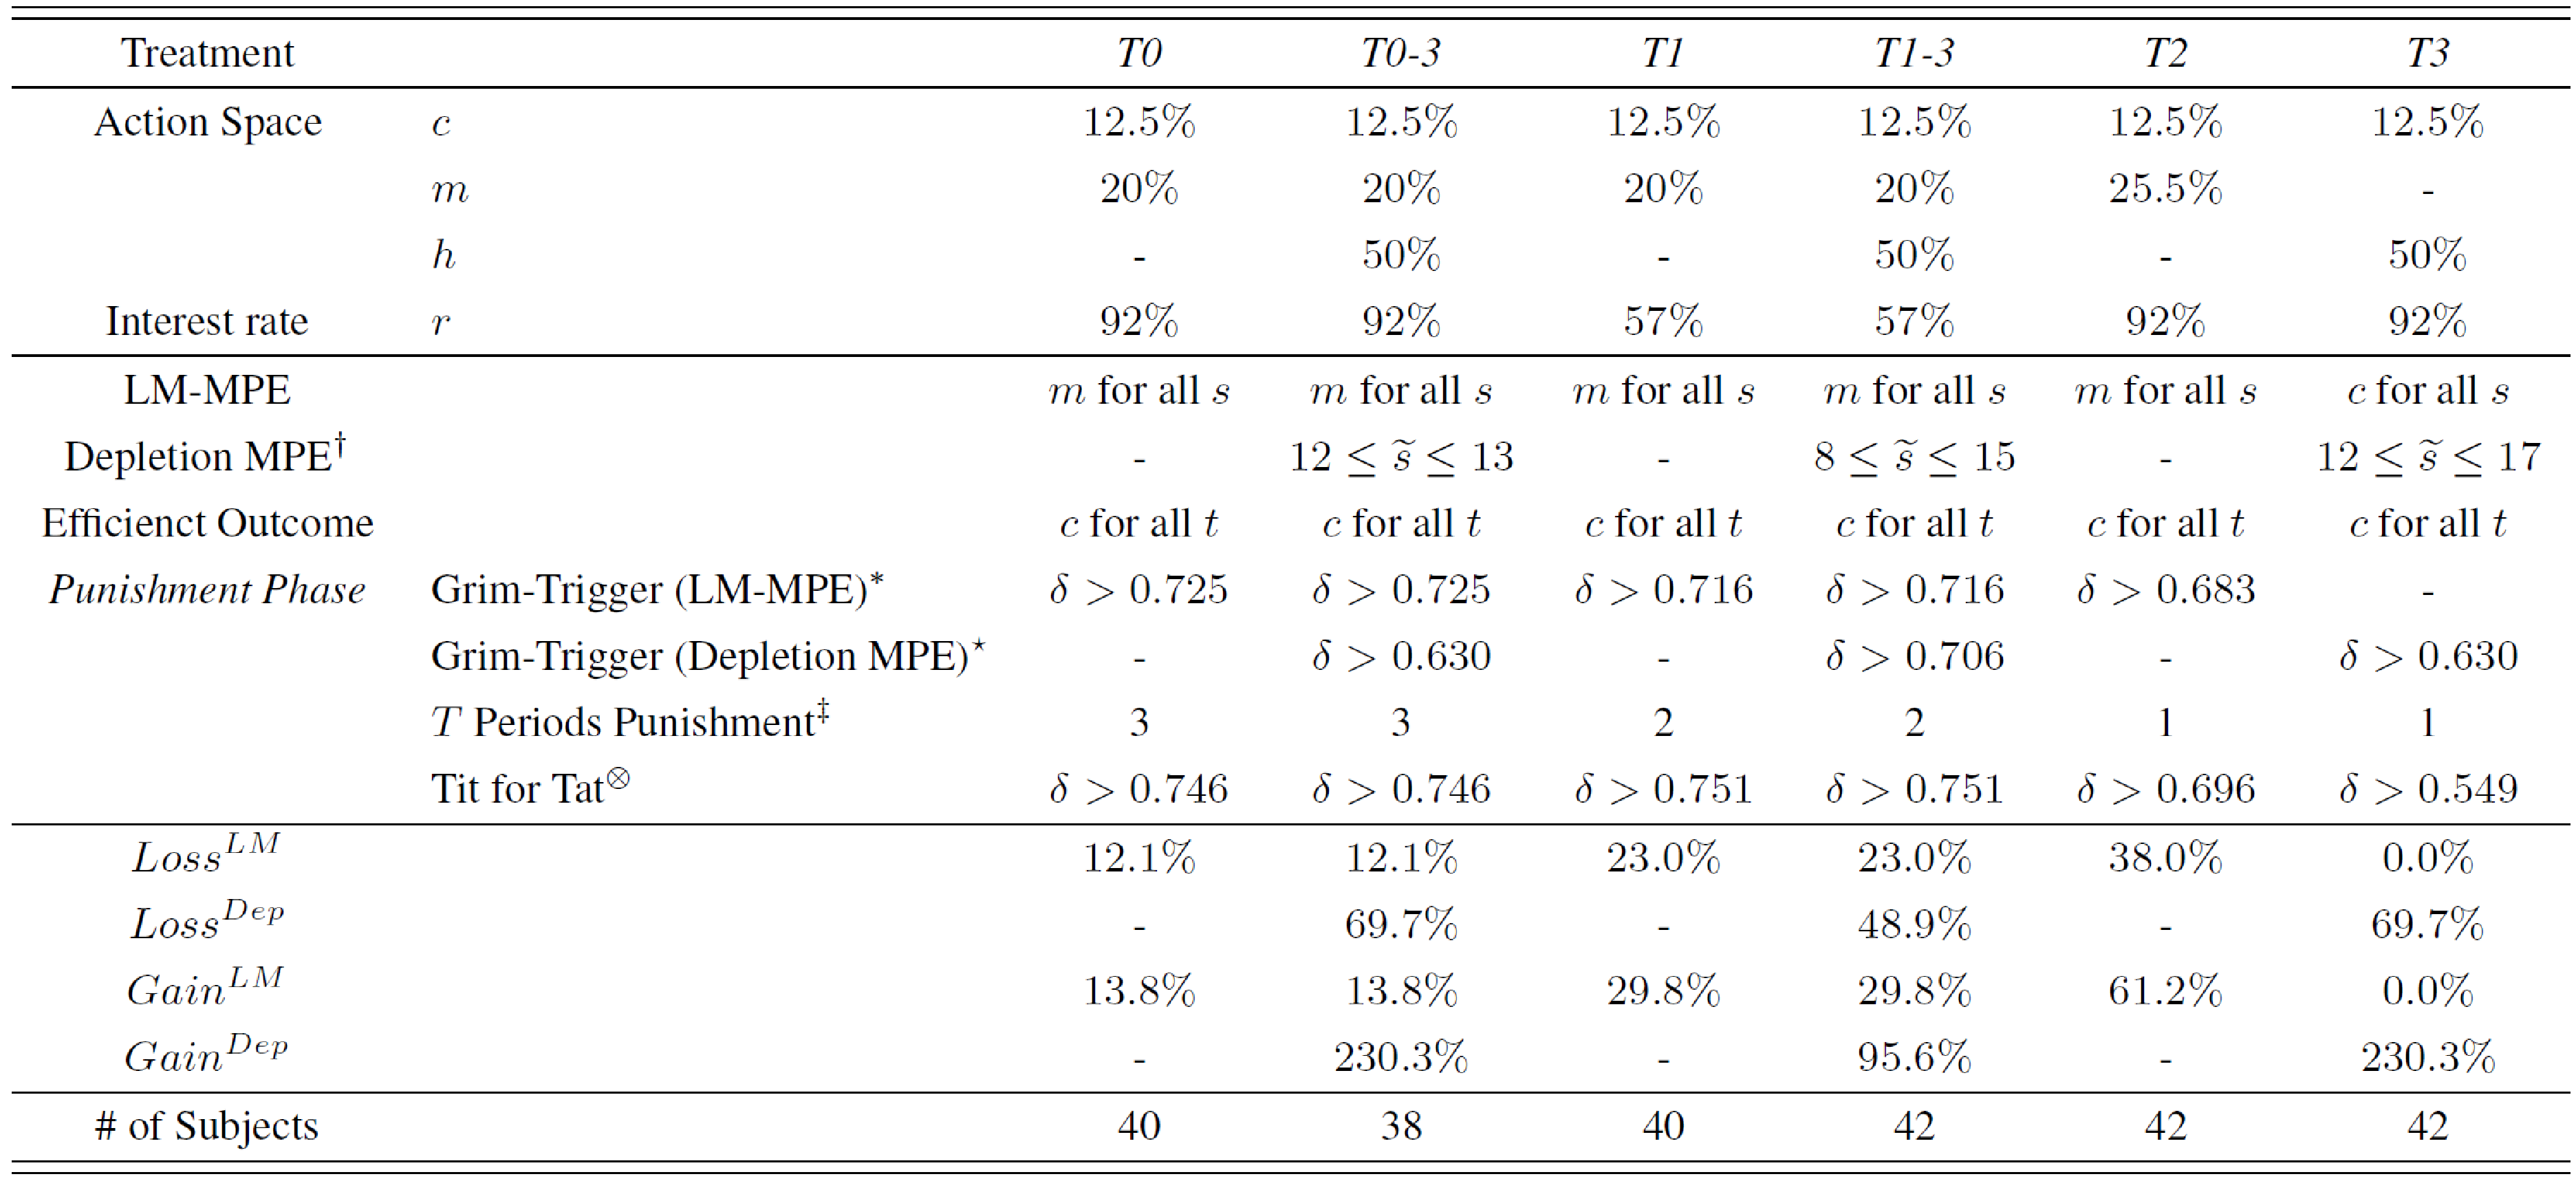
\includegraphics[width=1.0\textwidth]{../img/Vtbl1.pdf}
\end{center}
\end{frame}

\begin{frame}{Design Table}
\begin{center}
	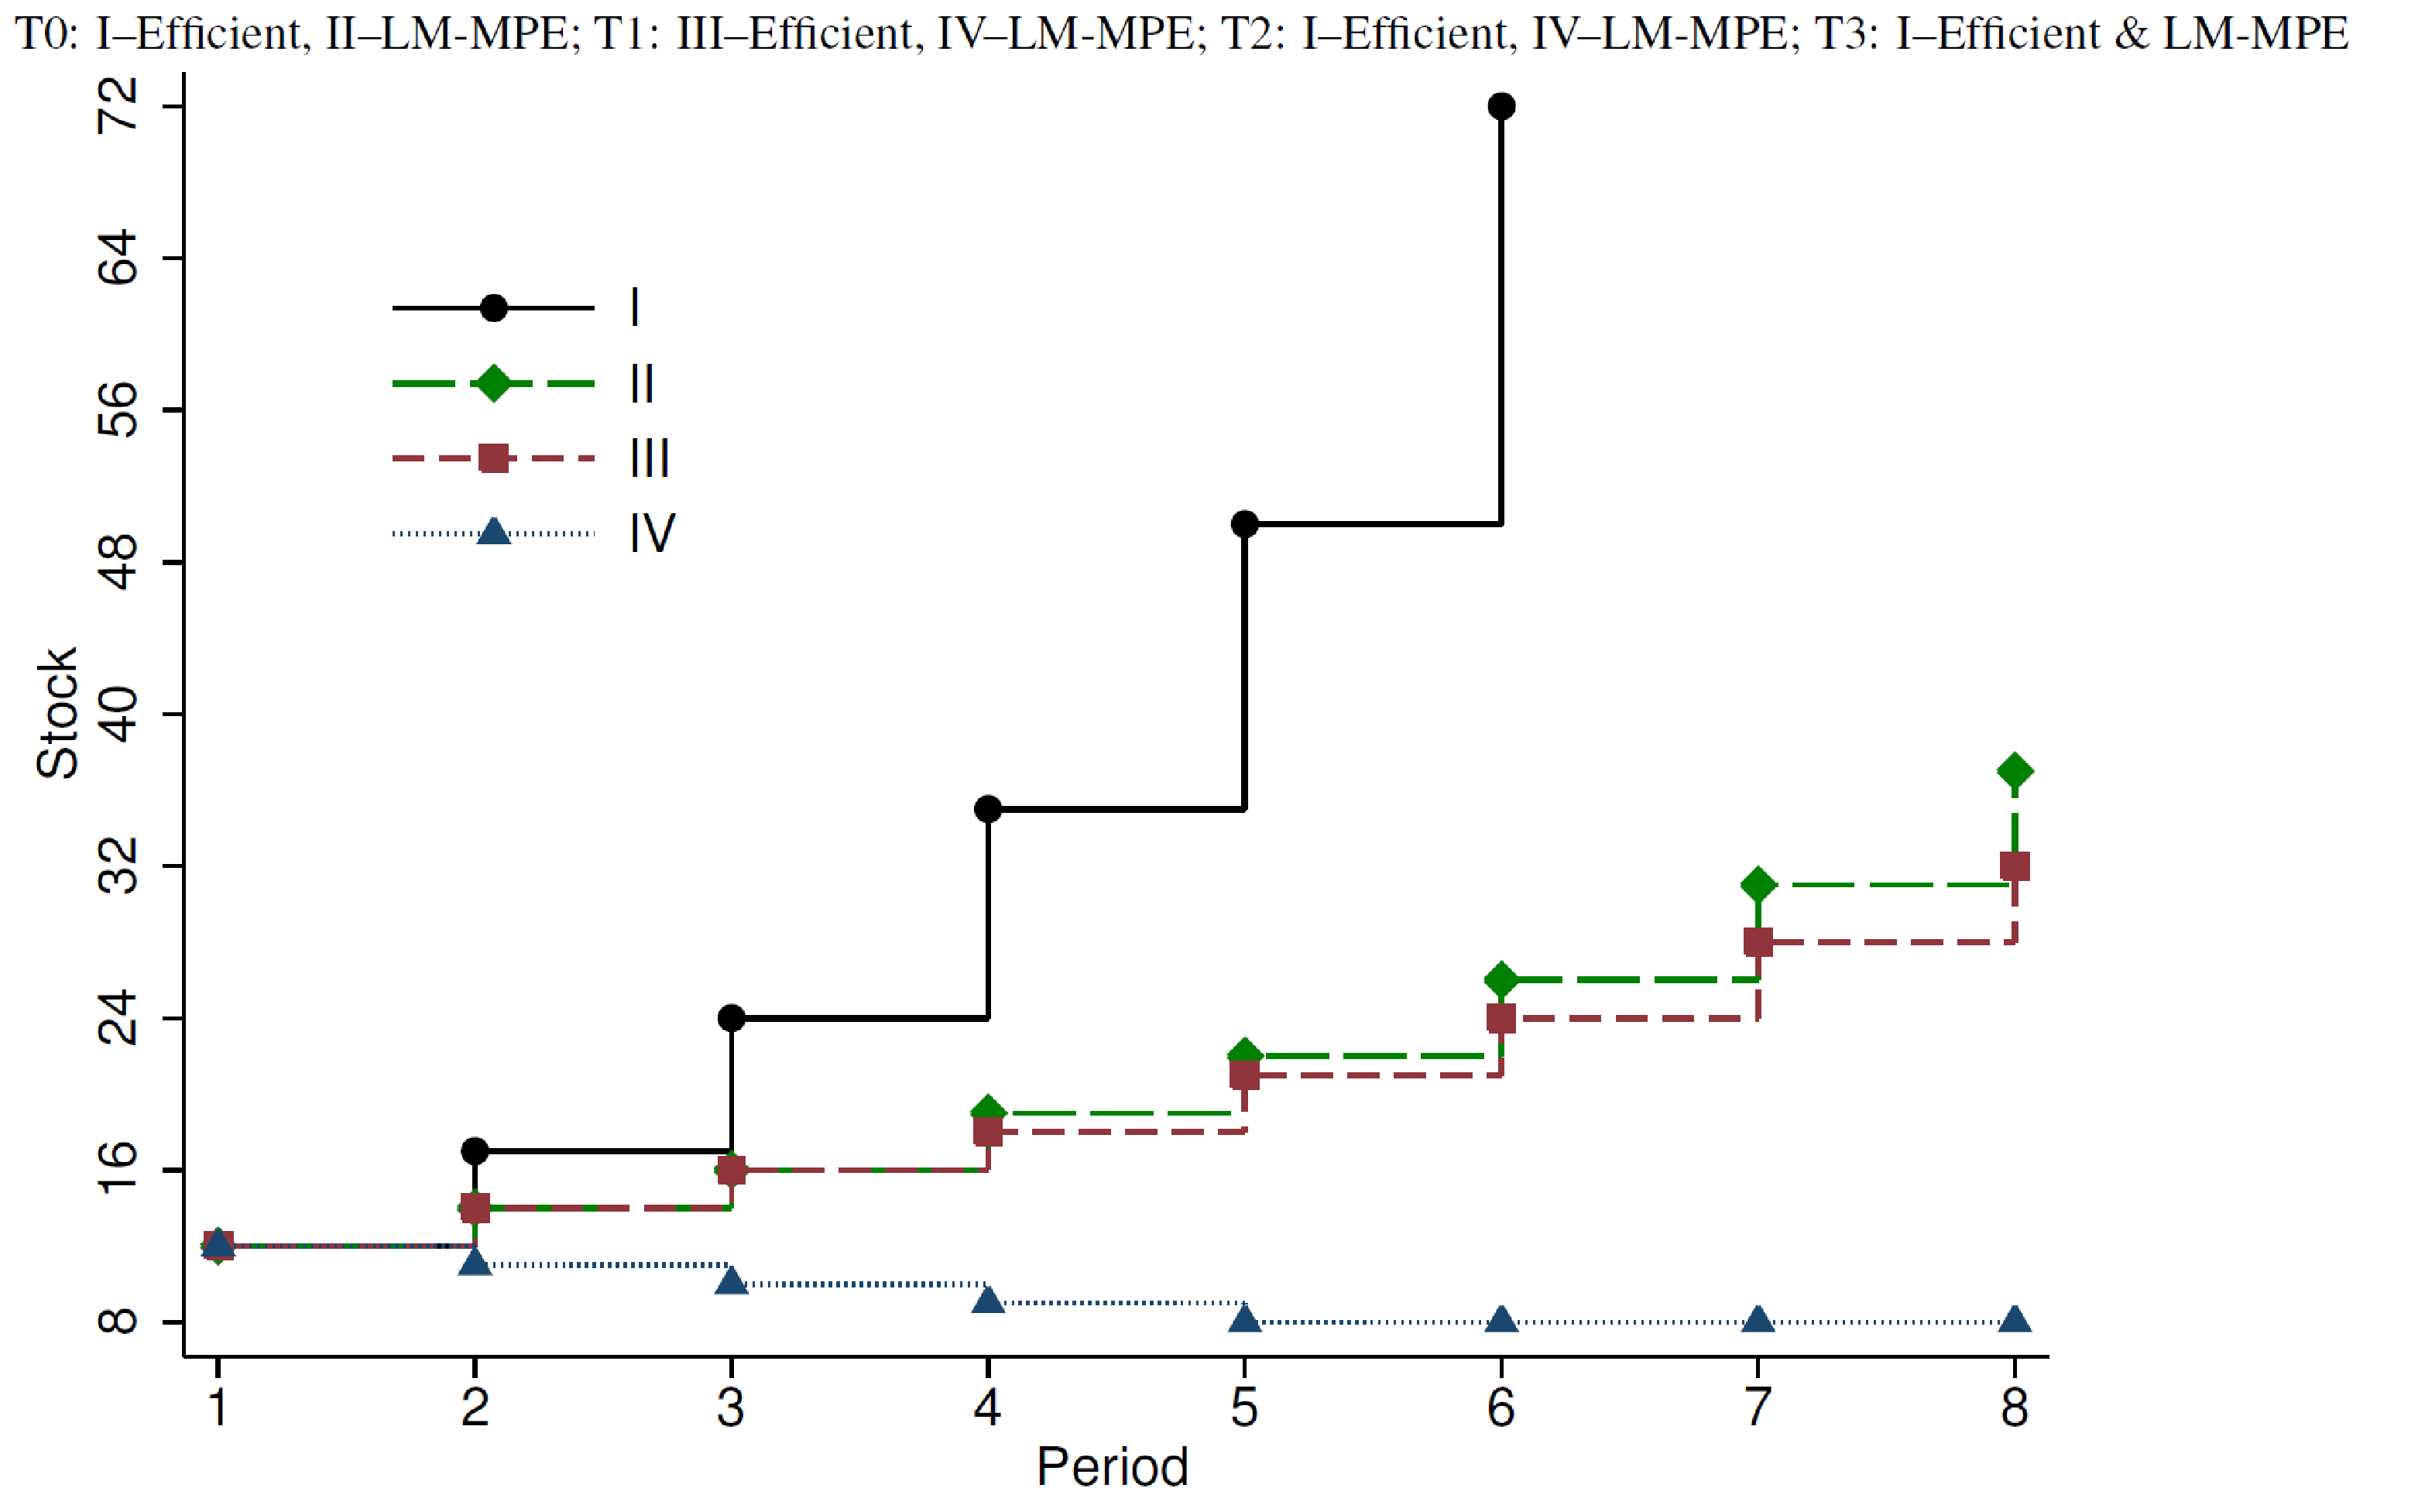
\includegraphics[width=1.0\textwidth]{../img/Vfig2.pdf}
\end{center}
\end{frame}

\begin{frame}{Interface}
\begin{center}
	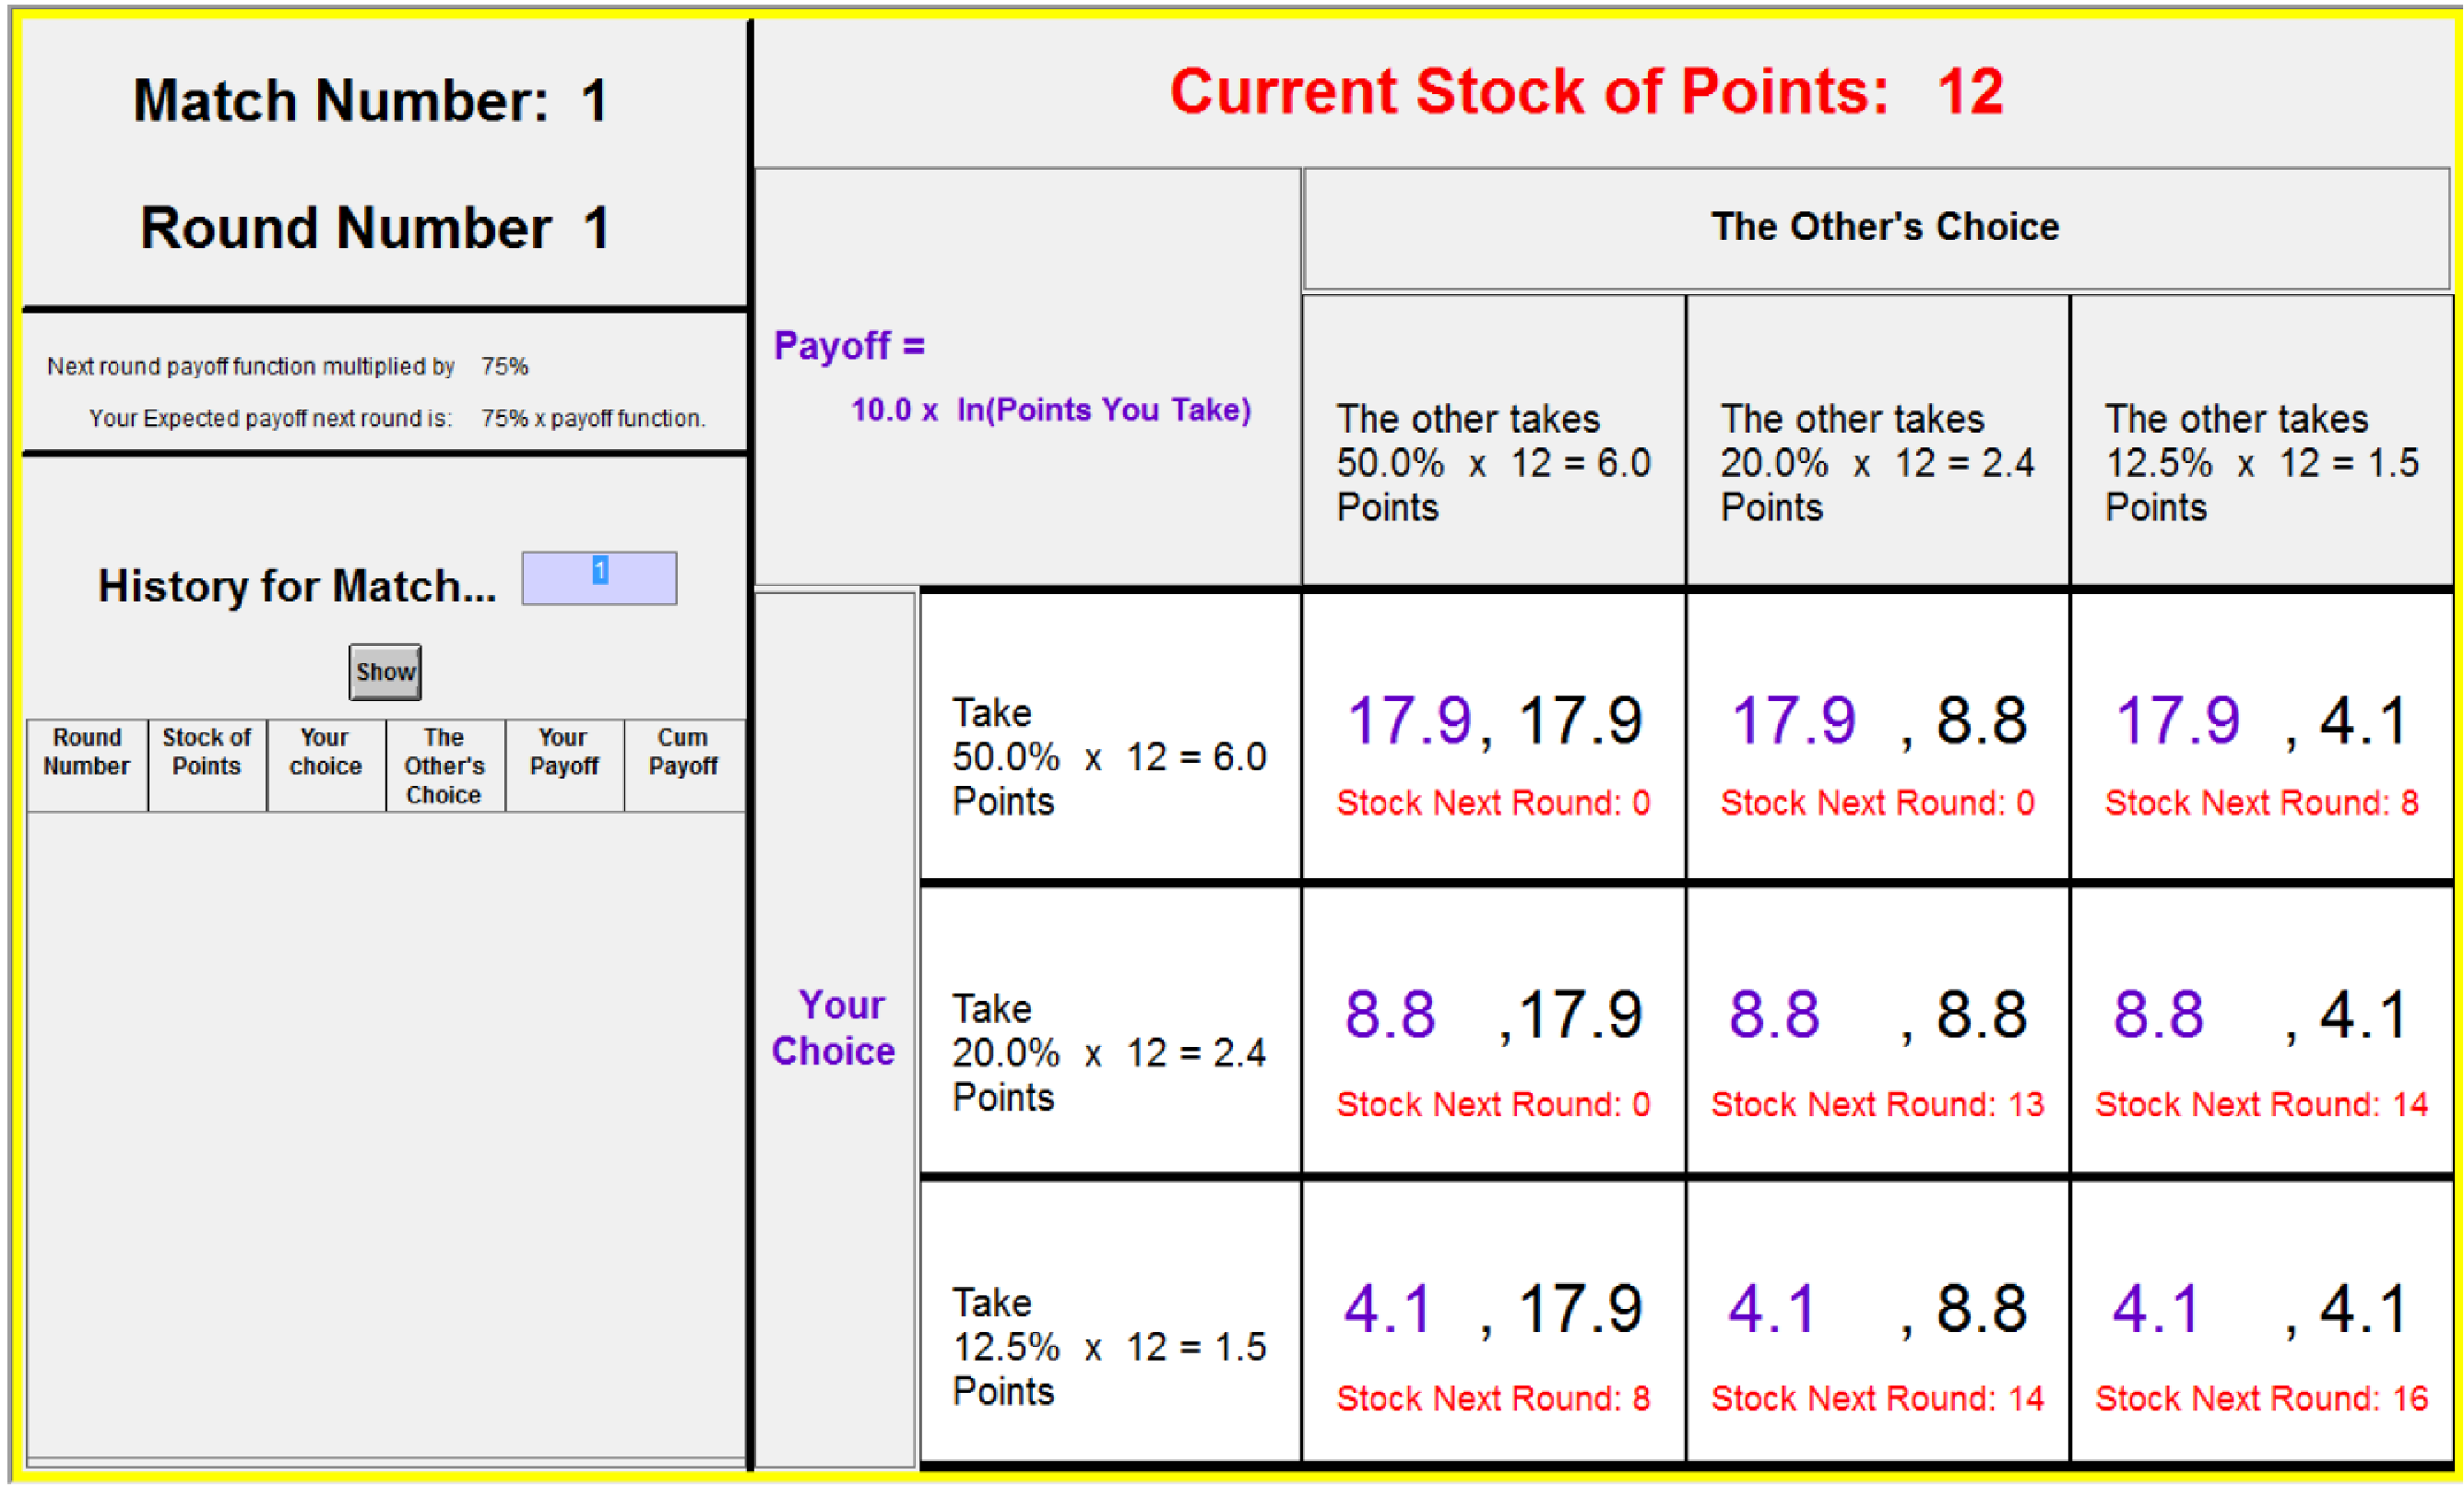
\includegraphics[width=0.9\textwidth]{../img/Vfig1a.pdf}
\end{center}
\end{frame}

\begin{frame}{Strategies used by subjects}
\begin{center}
	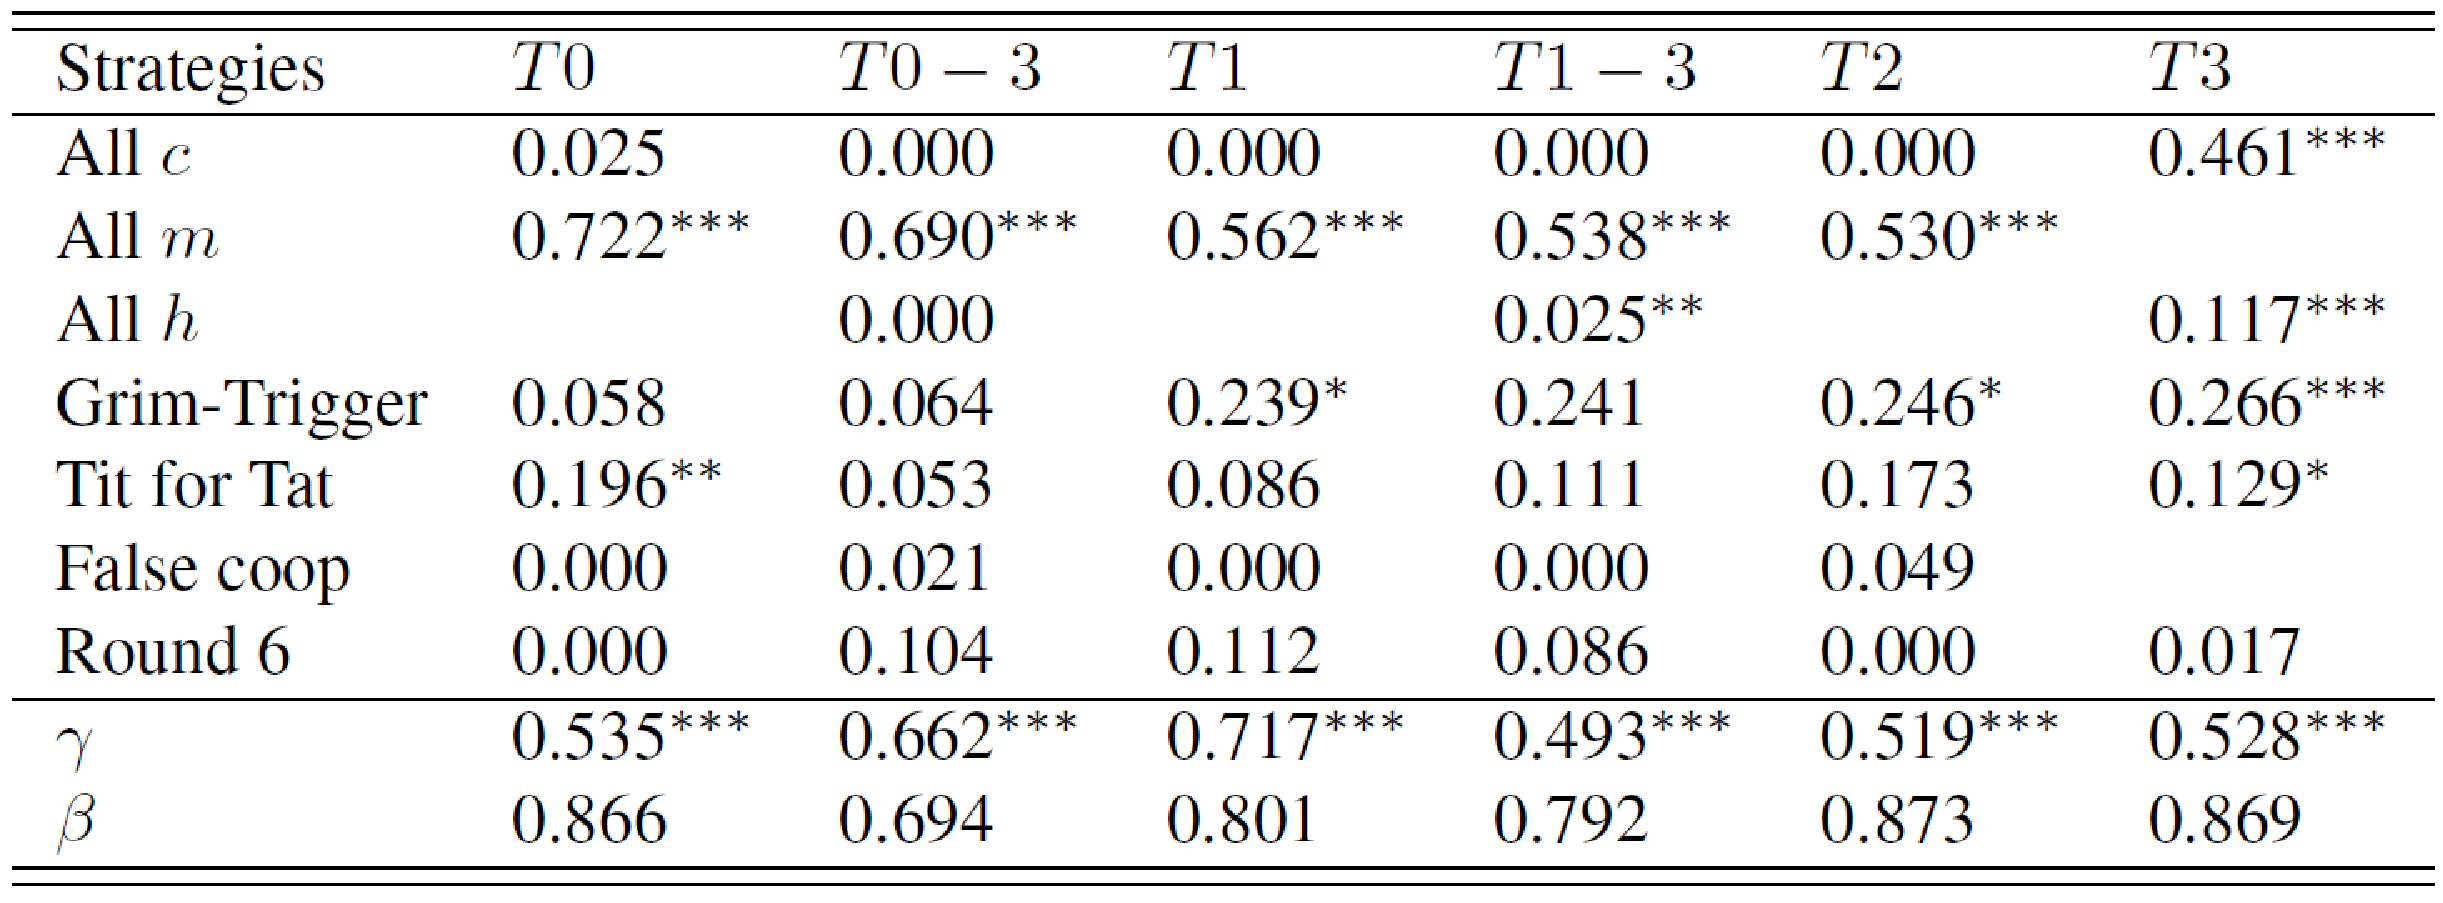
\includegraphics[width=0.9\textwidth]{../img/Vtbl3.pdf}
\end{center}
\begin{itemize}
	\item Estimated as mixture model
	\item MPE extraction is the most common strategy across treatments
\end{itemize}
\end{frame}

\begin{frame}{Vespa \& Wilson (2015) }

Connects behavior to the infinitely repeated
games literature.

Looks at the simplest dynamic game we could think of.

\begin{itemize}
\item Two agents, $\mathcal{I}=\left\{ 1,2\right\} $

\begin{itemize}
\item Two actions, $\mathcal{A}_{1}=\mathcal{A}_{2}$\only<1>{$=\left\{ \mbox{Cooperate},\mbox{Defect}\right\}$}\only<2>{$=\left\{ C,D \right\}$}
\item Two states, $\Omega$\only<1>{$=\left\{ \mbox{Low},\mbox{High}\right\}$}\only<2>{$=\left\{ L,H \right\}$} \pause
\end{itemize}
\item Any simpler in any variable and we would not have a dynamic game
\end{itemize}
\end{frame}


\begin{frame}{Fixed across environments}

\begin{itemize}
\item Infinite time horizon
\item Two agents: 1,2
\item Two states: \textcolor{red}{Low}, \textcolor{blue}{High}
\item Initial state: \textcolor{red}{Low}
\item Discounting: $\delta=75\%$\pause
\item Try to hold constant some of the strategic tensions
\end{itemize}
\end{frame}

\begin{frame}{Experimental Design}

\begin{itemize}
\item Three sessions per treatment
\item 14 subjects per session, EBEL-UCSB
\item 350 subjects total
\item Expected earnings: \$18 (between 75-90 minutes)
\item 15 repetitions of the supergame

\begin{itemize}
\item Going to call these cycles
\end{itemize}
\item Partial block design
\end{itemize}
\end{frame}


\begin{frame}{Structure of a session}

\begin{center}
\begin{tabular}{c|c|c|c|ccc|c|c|c|}
\multicolumn{1}{c}{} & \multicolumn{9}{c}{Cycle}\tabularnewline
\multirow{14}{*}{\begin{turn}{90}
Round
\end{turn}} & \textbf{\tiny{}1} & \textbf{\tiny{}2} & \textbf{\tiny{}3} & \multicolumn{3}{c|}{\textbf{\tiny{}...}} & \textbf{\tiny{}13} & \textbf{\tiny{}14} & \textbf{\tiny{}15}\tabularnewline
\cline{2-10}
 & \textbf{\textcolor{blue}{\tiny{}1}} & \textbf{\textcolor{blue}{\tiny{}1}} & \textbf{\textcolor{blue}{\tiny{}1}} &  &  &  & \textbf{\textcolor{blue}{\tiny{}1}} & \textbf{\textcolor{blue}{\tiny{}1}} & \textbf{\textcolor{blue}{\tiny{}1}}\tabularnewline
 & \textbf{\textcolor{blue}{\tiny{}2}} & \textbf{\textcolor{blue}{\tiny{}2}} & \textbf{\textcolor{blue}{\tiny{}2}} &  &  &  & \textbf{\tiny{}2} & \textbf{\textcolor{blue}{\tiny{}2}} & \textbf{\textcolor{blue}{\tiny{}2}}\tabularnewline
 & \textbf{\textcolor{blue}{\tiny{}3}} & \textbf{\tiny{}3} & \textbf{\textcolor{blue}{\tiny{}3}} &  &  &  & \textbf{\tiny{}3} & \textbf{\textcolor{blue}{\tiny{}3}} & \textbf{\textcolor{blue}{\tiny{}3}}\tabularnewline
 & \textbf{\textcolor{blue}{\tiny{}4}} & \textbf{\tiny{}4} & \textbf{\textcolor{blue}{\tiny{}4}} &  &  &  & \textbf{\tiny{}4} & \textbf{\textcolor{blue}{\tiny{}4}} & \textbf{\textcolor{blue}{\tiny{}4}}\tabularnewline
 & \textbf{\textcolor{blue}{\tiny{}5}} & \textbf{\tiny{}5} & \textbf{\textcolor{blue}{\tiny{}5}} &  &  &  & \textbf{\tiny{}5} & \textbf{\textcolor{blue}{\tiny{}5}} & \textbf{\textcolor{blue}{\tiny{}5}}\tabularnewline
 & \textbf{\textcolor{blue}{\tiny{}6}} &  & \textbf{\textcolor{blue}{\tiny{}6}} &  &  &  &  & \textbf{\textcolor{blue}{\tiny{}6}} & \tabularnewline
 & \textbf{\textcolor{blue}{\tiny{}7}} &  &  &  &  &  &  & \textbf{\textcolor{blue}{\tiny{}7}} & \tabularnewline
 & \textbf{\textcolor{blue}{\tiny{}8}} &  &  &  &  &  &  & \textbf{\textcolor{blue}{\tiny{}8}} & \tabularnewline
 &  &  &  &  &  &  &  & \textbf{\textcolor{blue}{\tiny{}9}} & \tabularnewline
 &  &  &  &  &  &  &  & \textbf{\textcolor{blue}{\tiny{}10}} & \tabularnewline
 &  &  &  &  &  &  &  & \textbf{\textcolor{blue}{\tiny{}11}} & \tabularnewline
 &  &  &  &  &  &  &  & \textbf{\textcolor{blue}{\tiny{}12}} & \tabularnewline
 &  &  &  &  &  &  &  & \textbf{\textcolor{blue}{\tiny{}13}} & \tabularnewline
\end{tabular}
\par\end{center}

\end{frame}
\begin{frame}


\begin{center}
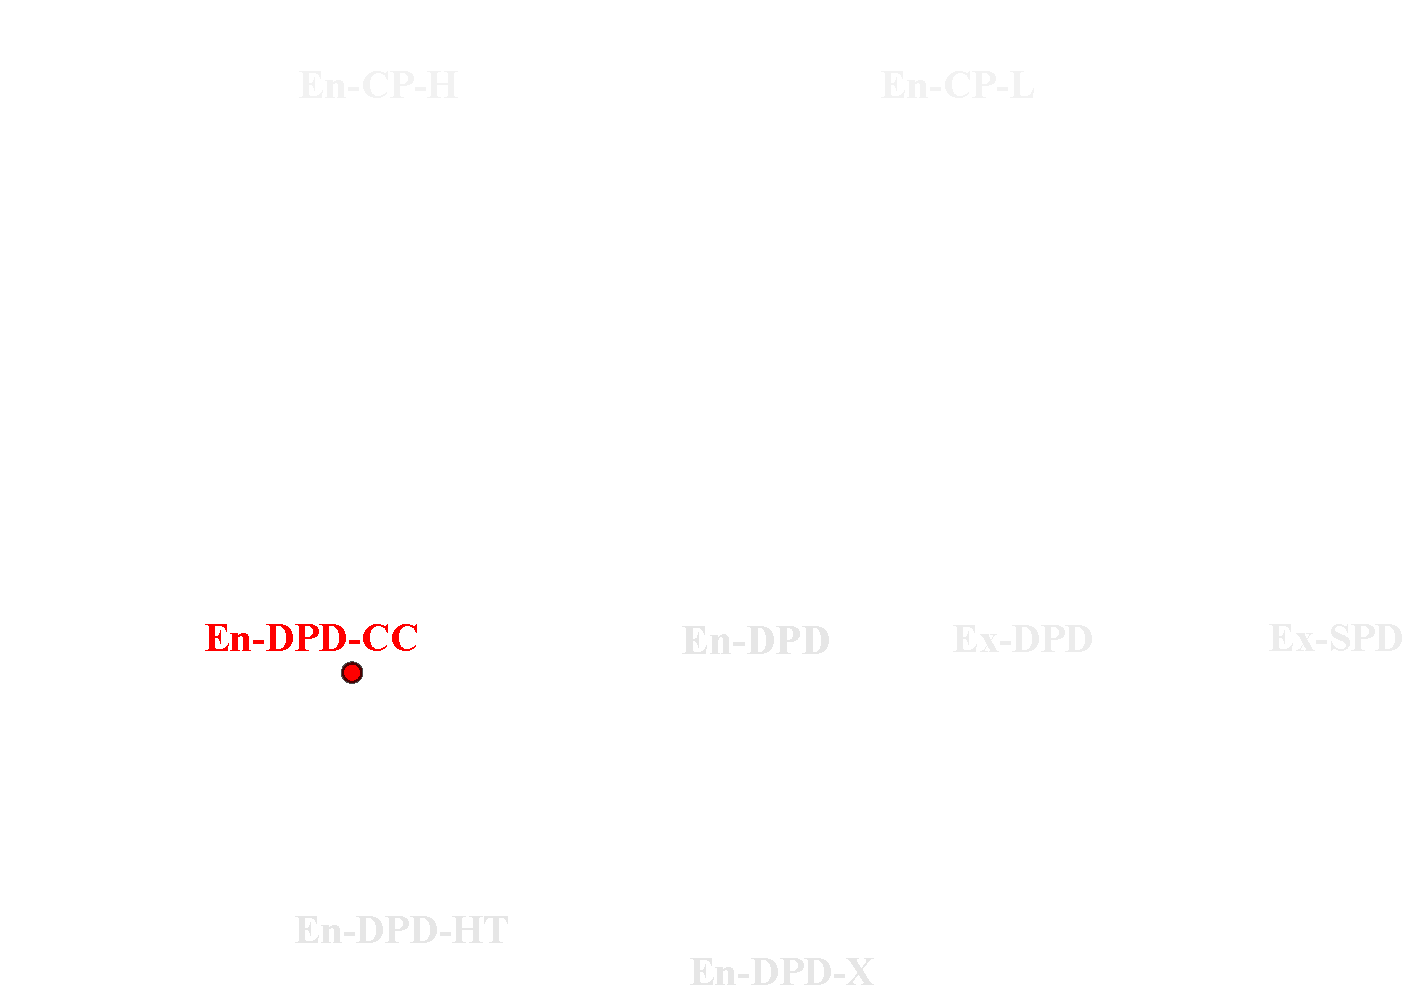
\includegraphics[height=0.7\textwidth]{../../../../p/vw_MPE/img/FlowChart1.pdf}
\end{center}
\end{frame}

\begin{frame}{Endogenous Dynamic PD-CC}


\begin{center}
\begin{table}
\centering{}\subfloat{\centering{}{\small{}}%
\begin{tabular}{cc>{\centering}p{0.14\textwidth}|>{\centering}p{0.14\textwidth}}
\multicolumn{4}{c}{\textcolor{red}{$\omega$=Low}}\tabularnewline
 &  & \multicolumn{1}{>{\centering}p{0.14\textwidth}}{} & \tabularnewline
 &  & \multicolumn{2}{c}{2}\tabularnewline
 &  & \multicolumn{1}{>{\centering}p{0.14\textwidth}}{\textbf{C}} & D\tabularnewline
\cline{3-4}
\multirow{2}{*}{1} & \multicolumn{1}{c|}{\textbf{C}} & \textcolor{blue}{100,100} & \multicolumn{1}{>{\centering}p{0.14\textwidth}|}{\textcolor{red}{30, 125}}\tabularnewline
\cline{3-4}
 & \multicolumn{1}{c|}{D} & \textcolor{red}{125, 30} & \multicolumn{1}{>{\centering}p{0.14\textwidth}|}{\textcolor{red}{60,60}}\tabularnewline
\cline{3-4}
\end{tabular}}\subfloat{\centering{}{\small{}}%
\begin{tabular}{cc>{\centering}p{0.14\textwidth}|>{\centering}p{0.15\textwidth}}
\multicolumn{4}{c}{\textcolor{blue}{$\omega$=High}}\tabularnewline
 &  & \multicolumn{1}{>{\centering}p{0.14\textwidth}}{} & \tabularnewline
 &  & \multicolumn{2}{c}{2}\tabularnewline
 &  & \multicolumn{1}{>{\centering}p{0.14\textwidth}}{C} & \textbf{D}\tabularnewline
\cline{3-4}
\multirow{2}{*}{1} & \multicolumn{1}{c|}{C} & \textcolor{blue}{200, 200} & \multicolumn{1}{>{\centering}p{0.15\textwidth}|}{\textcolor{blue}{130, 250}}\tabularnewline
\cline{3-4}
 & \multicolumn{1}{c|}{\textbf{D}} & \textcolor{blue}{250, 130} & \multicolumn{1}{>{\centering}p{0.15\textwidth}|}{\textbf{\textcolor{red}{190, 190}}}\tabularnewline
\cline{3-4}
\end{tabular}}
\end{table}

\par\end{center}


\textrm{
\[
\psi\left(\omega ,a \right)=\begin{cases}
\mbox{High} & \mbox{if }a=\left(C,C\right),\omega=\mbox{=Low}\\
\mbox{Low} & \mbox{if }a=\left(D,D\right), \omega=\mbox{\ensuremath{\omega}=High}\\
\omega & \mbox{otherwise}
\end{cases}
\]
}

\end{frame}


\begin{frame}{Dynamic PD Game CC: Graphical Representation}

\begin{center}
	\includegraphics<1>[width=0.6\textwidth]{../../../../p/vw_MPE/img/col_GamePayoffs1.pdf}
\end{center}

\end{frame}
\begin{frame}{Endogenous Dynamic PD-CC}


\begin{center}
\begin{table}
\centering{}\subfloat{\centering{}{\small{}}%
\begin{tabular}{cc>{\centering}p{0.1\textwidth}|>{\centering}p{0.1\textwidth}}
\multicolumn{4}{c}{\textcolor{red}{$\omega$=Low}}\tabularnewline
 &  & \multicolumn{1}{>{\centering}p{0.1\textwidth}}{} & \tabularnewline
 &  & \multicolumn{2}{c}{2}\tabularnewline
 &  & \multicolumn{1}{>{\centering}p{0.1\textwidth}}{\textbf{C}} & D\tabularnewline
\cline{3-4}
\multirow{2}{*}{1} & \multicolumn{1}{c|}{\textbf{C}} & \textcolor{blue}{100} & \multicolumn{1}{>{\centering}p{0.1\textwidth}|}{\textcolor{red}{30}}\tabularnewline
\cline{3-4}
 & \multicolumn{1}{c|}{D} & \textcolor{red}{125} & \multicolumn{1}{>{\centering}p{0.1\textwidth}|}{\textcolor{red}{60}}\tabularnewline
\cline{3-4}
\end{tabular}}\subfloat{\centering{}{\small{}}%
\begin{tabular}{cc>{\centering}p{0.1\textwidth}|>{\centering}p{0.1\textwidth}}
\multicolumn{4}{c}{\textcolor{blue}{$\omega$=High}}\tabularnewline
 &  & \multicolumn{1}{>{\centering}p{0.1\textwidth}}{} & \tabularnewline
 &  & \multicolumn{2}{c}{2}\tabularnewline
 &  & \multicolumn{1}{>{\centering}p{0.1\textwidth}}{C} & \textbf{D}\tabularnewline
\cline{3-4}
\multirow{2}{*}{1} & \multicolumn{1}{c|}{C} & \textcolor{blue}{200} & \multicolumn{1}{>{\centering}p{0.1\textwidth}|}{\textcolor{blue}{130}}\tabularnewline
\cline{3-4}
 & \multicolumn{1}{c|}{\textbf{D}} & \textcolor{blue}{250} & \multicolumn{1}{>{\centering}p{0.1\textwidth}|}{\textbf{\textcolor{red}{190}}}\tabularnewline
\cline{3-4}
\end{tabular}}
\end{table}

\par\end{center}


\textrm{
\[
\psi\left(\mbox{\ensuremath{\omega}},a\right)=\begin{cases}
\mbox{High} & \mbox{if }a=\left(C,C\right),\mbox{\ensuremath{\omega}=Low}\\
\mbox{Low} & \mbox{if }a=\left(D,D\right),\mbox{\ensuremath{\omega}=High}\\
\omega & \mbox{otherwise}
\end{cases}
\]
\pause}


Unique symmetric MPE: $\alpha_{i}^{\star}(\omega)=\begin{cases}
\mbox{C} & \mbox{if \ensuremath{\omega}=Low}\\
\mbox{D} & \mbox{if \ensuremath{\omega}=High}
\end{cases}$

\end{frame}

\begin{frame}{Other SPE?}


\begin{center}
\begin{table}
\centering{}\subfloat{\centering{}{\small{}}%
\begin{tabular}{cc>{\centering}p{0.1\textwidth}|>{\centering}p{0.1\textwidth}}
\multicolumn{4}{c}{\textcolor{red}{$\omega$=Low}}\tabularnewline
 &  & \multicolumn{1}{>{\centering}p{0.1\textwidth}}{} & \tabularnewline
 &  & \multicolumn{2}{c}{2}\tabularnewline
 &  & \multicolumn{1}{>{\centering}p{0.1\textwidth}}{\textbf{C}} & D\tabularnewline
\cline{3-4}
\multirow{2}{*}{1} & \multicolumn{1}{c|}{\textbf{C}} & \textcolor{blue}{100} & \multicolumn{1}{>{\centering}p{0.1\textwidth}|}{\textcolor{red}{30}}\tabularnewline
\cline{3-4}
 & \multicolumn{1}{c|}{D} & \textcolor{red}{125} & \multicolumn{1}{>{\centering}p{0.1\textwidth}|}{\textcolor{red}{60}}\tabularnewline
\cline{3-4}
\end{tabular}}\subfloat{\centering{}{\small{}}%
\begin{tabular}{cc>{\centering}p{0.1\textwidth}|>{\centering}p{0.1\textwidth}}
\multicolumn{4}{c}{\textcolor{blue}{$\omega$=High}}\tabularnewline
 &  & \multicolumn{1}{>{\centering}p{0.1\textwidth}}{} & \tabularnewline
 &  & \multicolumn{2}{c}{2}\tabularnewline
 &  & \multicolumn{1}{>{\centering}p{0.1\textwidth}}{C} & \textbf{D}\tabularnewline
\cline{3-4}
\multirow{2}{*}{1} & \multicolumn{1}{c|}{C} & \textcolor{blue}{200} & \multicolumn{1}{>{\centering}p{0.1\textwidth}|}{\textcolor{blue}{130}}\tabularnewline
\cline{3-4}
 & \multicolumn{1}{c|}{\textbf{D}} & \textcolor{blue}{250} & \multicolumn{1}{>{\centering}p{0.1\textwidth}|}{\textbf{\textcolor{red}{190}}}\tabularnewline
\cline{3-4}
\end{tabular}}
\end{table}

\par\end{center}
\begin{itemize}
\item Many other SPE

\begin{itemize}
\item Can sustain efficient outcome $(C,C)$ using history-dependent strategies
\end{itemize}
\end{itemize}
\end{frame}


\begin{frame}{MPE in En-DPD-CC}

\begin{itemize}\item If the MPE is selected we should expect to see
		\begin{itemize}
			\item Full cooperation in low state
			\item No cooperation in high state
			\item No difference in rate of cooperation through the cycle
		\end{itemize}
\end{itemize}
\end{frame}

\begin{frame}{Results: Cooperation by State}

\begin{center}
	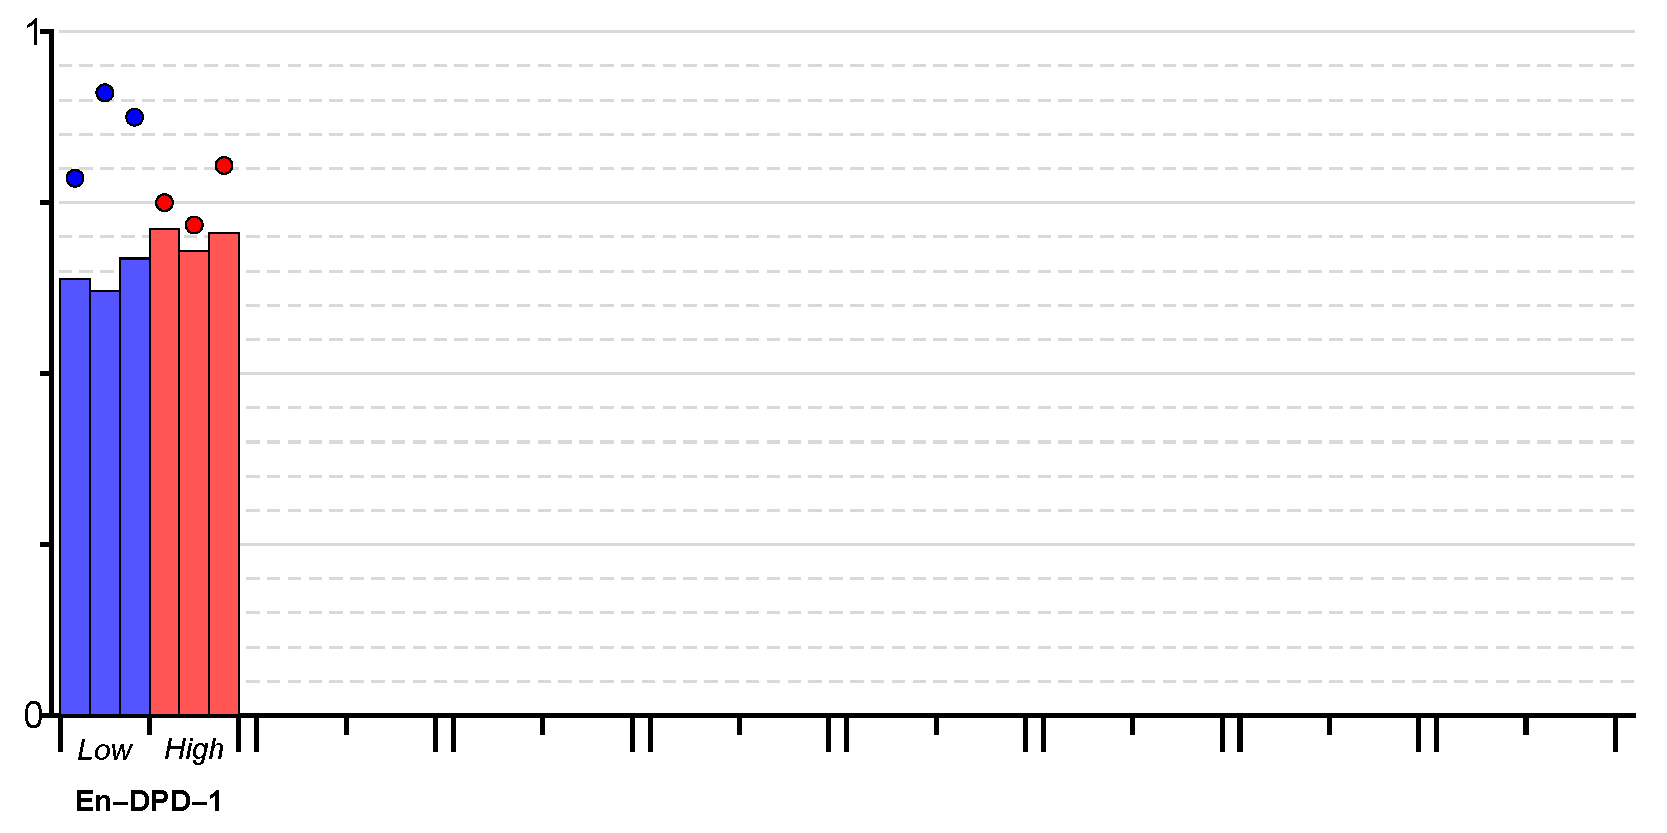
\includegraphics[width=1.0\textwidth]{../../../../p/vw_MPE/img/col_bar_StateCoop_block_EnDPD_1.pdf}
\end{center}

{\small \begin{itemize}\item Points indicate Cooperation rate in first/second round for low/high state
\item Blocks of cycles 1--5, 6--10, 11--15
\end{itemize}
}\end{frame}
\begin{frame}{Subject Cooperation }


\begin{center}
	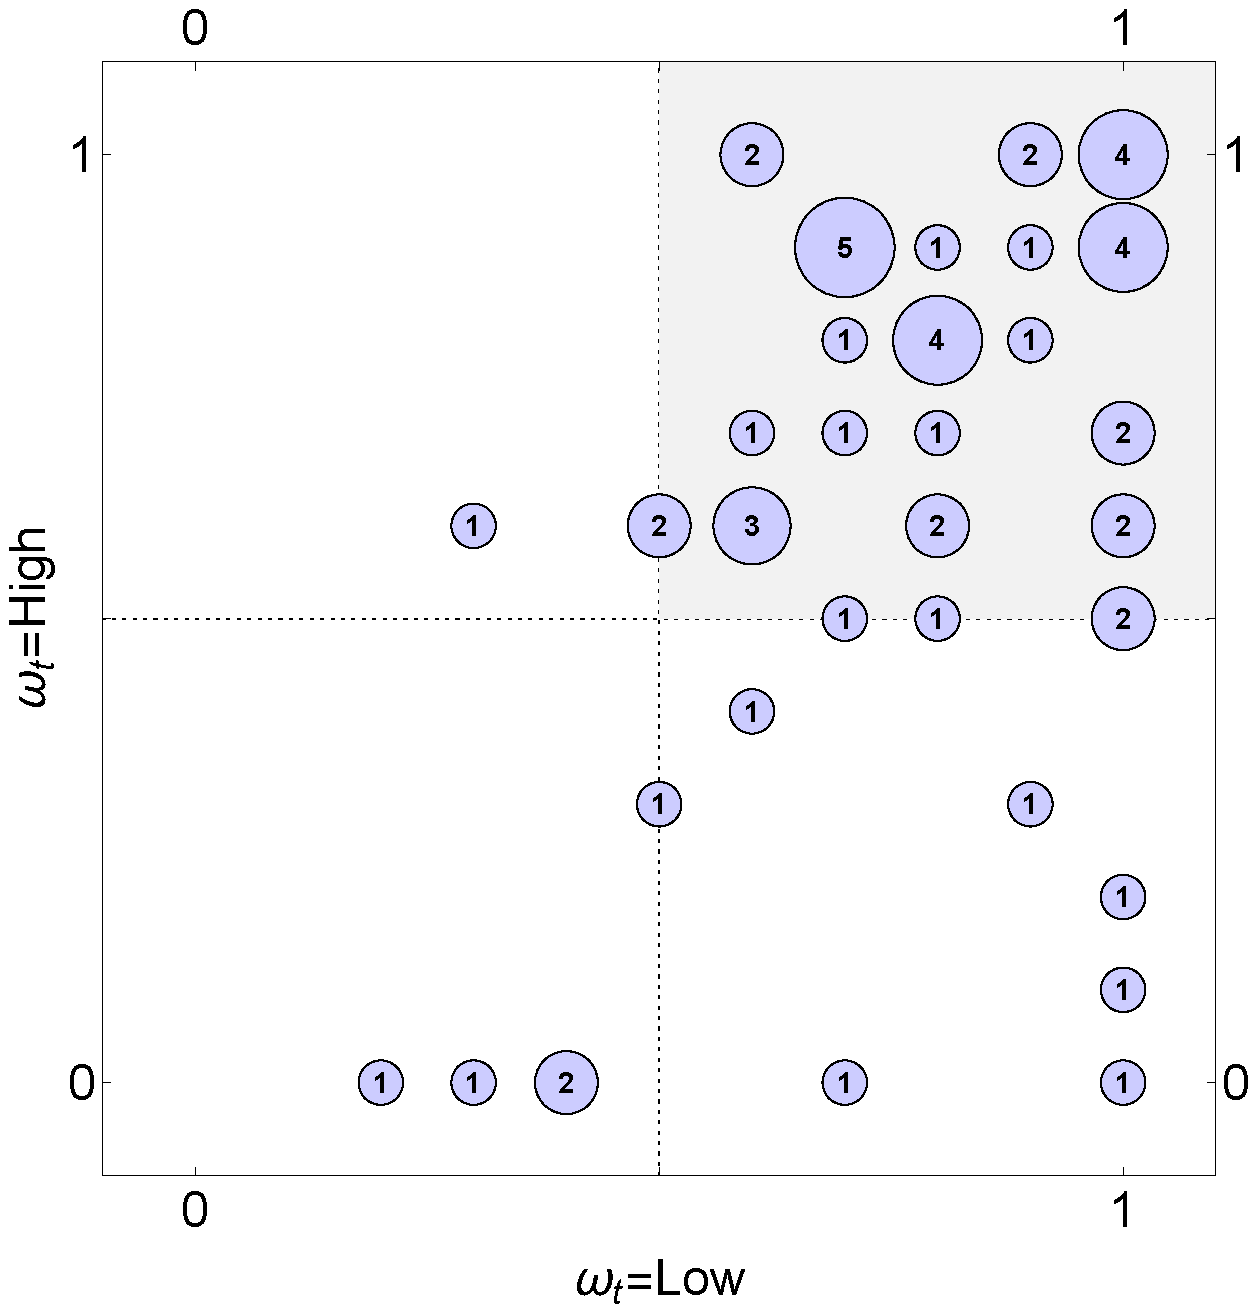
\includegraphics[width=0.6\textwidth]{../../../../p/vw_MPE/img/col_subject_stateCooperation_L5_EnDPD_1.pdf}
\end{center}

\end{frame}

\begin{frame}{Sequences}

\begin{itemize}
\item Most popular sequences across rounds 11--15 are:

\begin{itemize}
\item \textcolor{red}{CC},\textcolor{blue}{CC},\textcolor{blue}{CC},\textcolor{blue}{CC},\textcolor{blue}{CC}
(26\% of cycles)
\item \textcolor{red}{CC},\textcolor{blue}{CC},\textcolor{blue}{CC},\textcolor{blue}{DC},\textcolor{blue}{DD}
(8\% of cycles)
\item \textcolor{red}{CC},\textcolor{blue}{CC},\textcolor{blue}{CC},\textcolor{blue}{CC},\textcolor{blue}{DC}
(5\% of cycles)
\end{itemize}
\item Looks somewhat cooperative

\begin{itemize}
\item 61\% of cycles stay in High state in periods 2--5
\item 12\% of cycles never get out of Low state
\item Only 3\% of cycles alternate Low, High, Low, ...
\item Only 2\% of cycles never reach High state
\end{itemize}
\end{itemize}
\end{frame}

\begin{frame}{Subject-level Response}

\begin{itemize}
\item Subject in Ex-DPD: \only<1>{Subject Always Defect}
\only<2>{Subject somewhat Markov}
\only<3>{Subject Grim-like}
\only<4>{Subject Markov-trigger}
\end{itemize}

\begin{center}
\includegraphics<1>[height=0.5\textheight]{../../../../p/vw_MPE/img/subject/EnDPD_11.pdf}
\includegraphics<2>[height=0.5\textheight]{../../../../p/vw_MPE/img/subject/EnDPD_112.pdf}
\includegraphics<3>[height=0.5\textheight]{../../../../p/vw_MPE/img/subject/EnDPD_146.pdf}
\includegraphics<4>[height=0.5\textheight]{../../../../p/vw_MPE/img/subject/EnDPD_125.pdf}
\end{center}


\end{frame}

\begin{frame}{Strategies}

\begin{itemize}
\item Estimate using SFEM mixture model
\item Popular pure strategy Markov:

\begin{itemize}
\item C-C 14.9\%
\item C-D 7.4\% (the MPE)
\item D-D/D-C 7.1\%
\end{itemize}
\item Popular history-dependent strategies

\begin{itemize}
\item Grim trigger 19.2\%
\item C-Alternate-in-high, grim trigger 20.7\%
\end{itemize}
\end{itemize}
\end{frame}

\begin{frame}


\textbf{Result 1: }



\textbf{Not all dynamic games lead to the selection of MPE outcomes;
still observe a lot of conditional cooperation}
\end{frame}

\begin{frame}


\begin{center}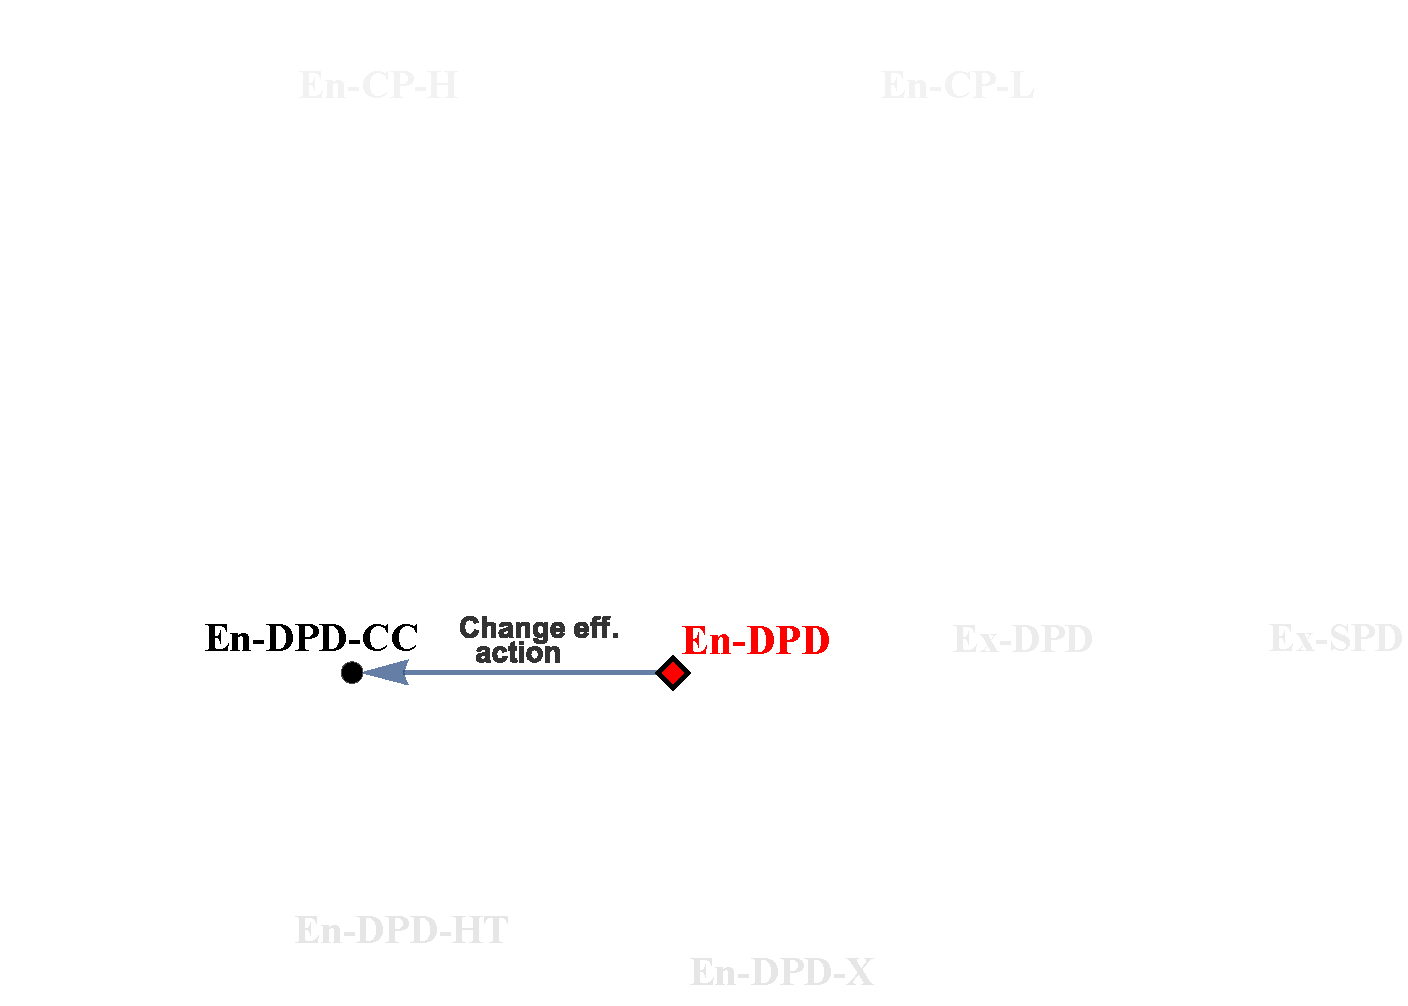
\includegraphics[height=0.7\textwidth]{../../../../p/vw_MPE/img/FlowChart2.pdf}
\end{center}
\end{frame}


\begin{frame}{En-DPD-CC $\rightarrow$ En-DPD}
\begin{itemize}
\item \textbf{Manipulation 1:} Alter the efficient frontier in high

\begin{itemize}
\item Increase temptation to defect in high
\item Make efficient action harder: C/D alternation in high
\end{itemize}
\end{itemize}
\end{frame}
\begin{frame}{Endog-Dynamic-PD (Pivot)}


\begin{center}
\begin{table}
\centering{}\subfloat{\centering{}{\small{}}%
\begin{tabular}{cc>{\centering}p{0.1\textwidth}|>{\centering}p{0.1\textwidth}}
\multicolumn{4}{c}{\textcolor{red}{$\omega$=Low}}\tabularnewline
 &  & \multicolumn{1}{>{\centering}p{0.1\textwidth}}{} & \tabularnewline
 &  & \multicolumn{2}{c}{2}\tabularnewline
 &  & \multicolumn{1}{>{\centering}p{0.1\textwidth}}{\textbf{C}} & D\tabularnewline
\cline{3-4}
\multirow{2}{*}{1} & \multicolumn{1}{c|}{\textbf{C}} & \textcolor{blue}{100} & \multicolumn{1}{>{\centering}p{0.1\textwidth}|}{\textcolor{red}{30}}\tabularnewline
\cline{3-4}
 & \multicolumn{1}{c|}{D} & \textcolor{red}{125} & \multicolumn{1}{>{\centering}p{0.1\textwidth}|}{\textcolor{red}{60}}\tabularnewline
\cline{3-4}
\end{tabular}}\subfloat{\centering{}{\small{}}%
\begin{tabular}{cc>{\centering}p{0.1\textwidth}|>{\centering}p{0.1\textwidth}}
\multicolumn{4}{c}{\textcolor{blue}{$\omega$=High}}\tabularnewline
 &  & \multicolumn{1}{>{\centering}p{0.1\textwidth}}{} & \tabularnewline
 &  & \multicolumn{2}{c}{2}\tabularnewline
 &  & \multicolumn{1}{>{\centering}p{0.1\textwidth}}{C} & \textbf{D}\tabularnewline
\cline{3-4}
\multirow{2}{*}{1} & \multicolumn{1}{c|}{C} & \textcolor{blue}{200} & \multicolumn{1}{>{\centering}p{0.1\textwidth}|}{\textcolor{blue}{130}}\tabularnewline
\cline{3-4}
 & \multicolumn{1}{c|}{\textbf{D}} & \textcolor{blue}{\only<1>{250}\only<2>{280}} & \multicolumn{1}{>{\centering}p{0.1\textwidth}|}{\textbf{\textcolor{red}{190}}}\tabularnewline
\cline{3-4}
\end{tabular}}
\end{table}

\par\end{center}


\textrm{
\[
\psi\left(\mbox{\ensuremath{\omega}},a\right)=\begin{cases}
\mbox{High} & \mbox{if }a=\left(C,C\right),\mbox{\ensuremath{\omega}=Low}\\
\mbox{Low} & \mbox{if }a=\left(D,D\right),\mbox{\ensuremath{\omega}=High}\\
\omega & \mbox{otherwise}
\end{cases}
\]
\pause}


Unique MPE still: $\alpha_{i}^{\star}(\omega)=\begin{cases}
\mbox{C} & \mbox{if \ensuremath{\omega}=Low}\\
\mbox{D} & \mbox{if \ensuremath{\omega}=High}
\end{cases}$

\end{frame}


\begin{frame}{Dynamic PD Game-\only<1>{1}\only<2>{2}}

\begin{center}
	\includegraphics<1>[width=0.6\textwidth]{../../../../p/vw_MPE/img/col_GamePayoffs1.pdf}
	\includegraphics<2>[width=0.6\textwidth]{../../../../p/vw_MPE/img/col_GamePayoffs2.pdf}
\end{center}

\end{frame}

\begin{frame}{Results: Cooperation by State}

\begin{center}
	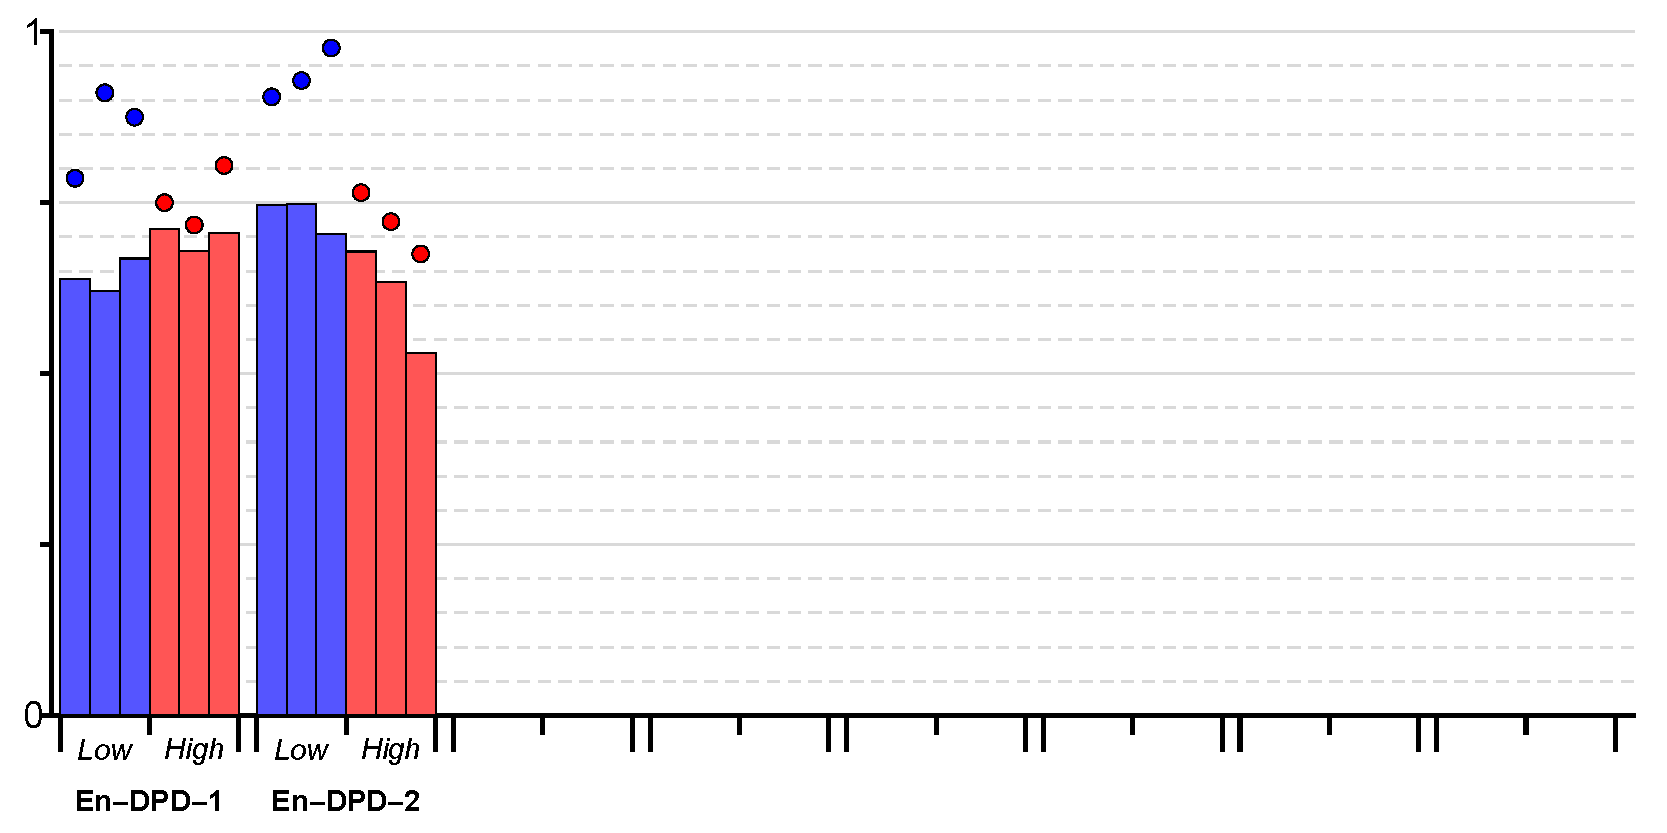
\includegraphics[width=1.0\textwidth]{../../../../p/vw_MPE/img/col_bar_StateCoop_block_EnDPD_2.pdf}
\end{center}

{\small \begin{itemize}\item Points indicate Cooperation rate in first/second round for low/high state
\item Blocks of cycles 1--5, 6--10, 11--15
\end{itemize}
}\end{frame}
\begin{frame}{Subject Cooperation:En-DPD-CC$\rightarrow$\only<2>{En-DPD} }


\begin{center}
	\includegraphics<1>[width=0.6\textwidth]{../../../../p/vw_MPE/img/col_subject_stateCooperation_L5_EnDPD_1.pdf}
	\includegraphics<2>[width=0.6\textwidth]{../../../../p/vw_MPE/img/col_subject_stateCooperation_L5_EnDPD_2.pdf}
\end{center}

\end{frame}

% \begin{frame}{Sequences}

% \begin{itemize}
% \item Most popular sequences across rounds 1--5 are:

% \begin{itemize}
% \item \textcolor{red}{CC},\textcolor{blue}{DC},\textcolor{blue}{DD},\textcolor{red}{CC},\textcolor{blue}{DD}(10\%
% of cycles)
% \item \textcolor{red}{CC},\textcolor{blue}{CC},\textcolor{blue}{CC},\textcolor{blue}{CC},\textcolor{blue}{CC}
% (9\% of cycles)
% \item \textcolor{red}{CC},\textcolor{blue}{CC},\textcolor{blue}{CC},\textcolor{blue}{CC},\textcolor{blue}{DC}
% (6\% of cycles)
% \end{itemize}
% \item Attempts at cooperation

% \begin{itemize}
% \item 48\% of cycles stay in High state in periods 2--5
% \item Only 4\% of cycles alternate Low, High, Low, ...
% \item Only 4\% of cycles never reach High state.
% \end{itemize}
% \end{itemize}
% \end{frame}

\begin{frame}{Strategies}

\begin{itemize}
\item Popular pure strategy Markov:

\begin{itemize}
\item C-C: $14.9\%\rightarrow7.9\%$
\item C-D: $7.1\%\rightarrow23.5\%$
\item D-D: $7.4\%\rightarrow4.7\%$
\end{itemize}
\item Popular history-dependent strategies

\begin{itemize}
\item Grim trigger $19.2\%\rightarrow13.8\%$
\item C-Alternate-in-high, grim trigger $20.7\%\rightarrow0\%$
\item D-Alternate-in-high, grim trigger $1.5\%\rightarrow16.2\%$
\item C-Alternate-in-high, MPE-trigger $5.8\%\rightarrow28.7\%$
\end{itemize}
\item \textbf{More Markov; More alternation; Markov-triggers over grim}
\end{itemize}
\end{frame}

\begin{frame}{Subject-level Response}

\begin{itemize}
\item Subject in Ex-DPD: \only<1>{Subject D-Alternate-Grim trigger}
\only<2>{Subject C-Alternate Markov trigger}
\end{itemize}

\begin{center}
\includegraphics<1>[height=0.5\textheight]{../../../../p/vw_MPE/img/subject/EnDPD_218.pdf}
\includegraphics<2>[height=0.5\textheight]{../../../../p/vw_MPE/img/subject/EnDPD_227.pdf}
\end{center}
\end{frame}

\begin{frame}


\textbf{Result 2: }



\textbf{Conditional cooperation here moves to support the efficient
outcome, though C/D alternation in High was common even when joint
cooperation was efficient}
\end{frame}

\begin{frame}


\begin{center}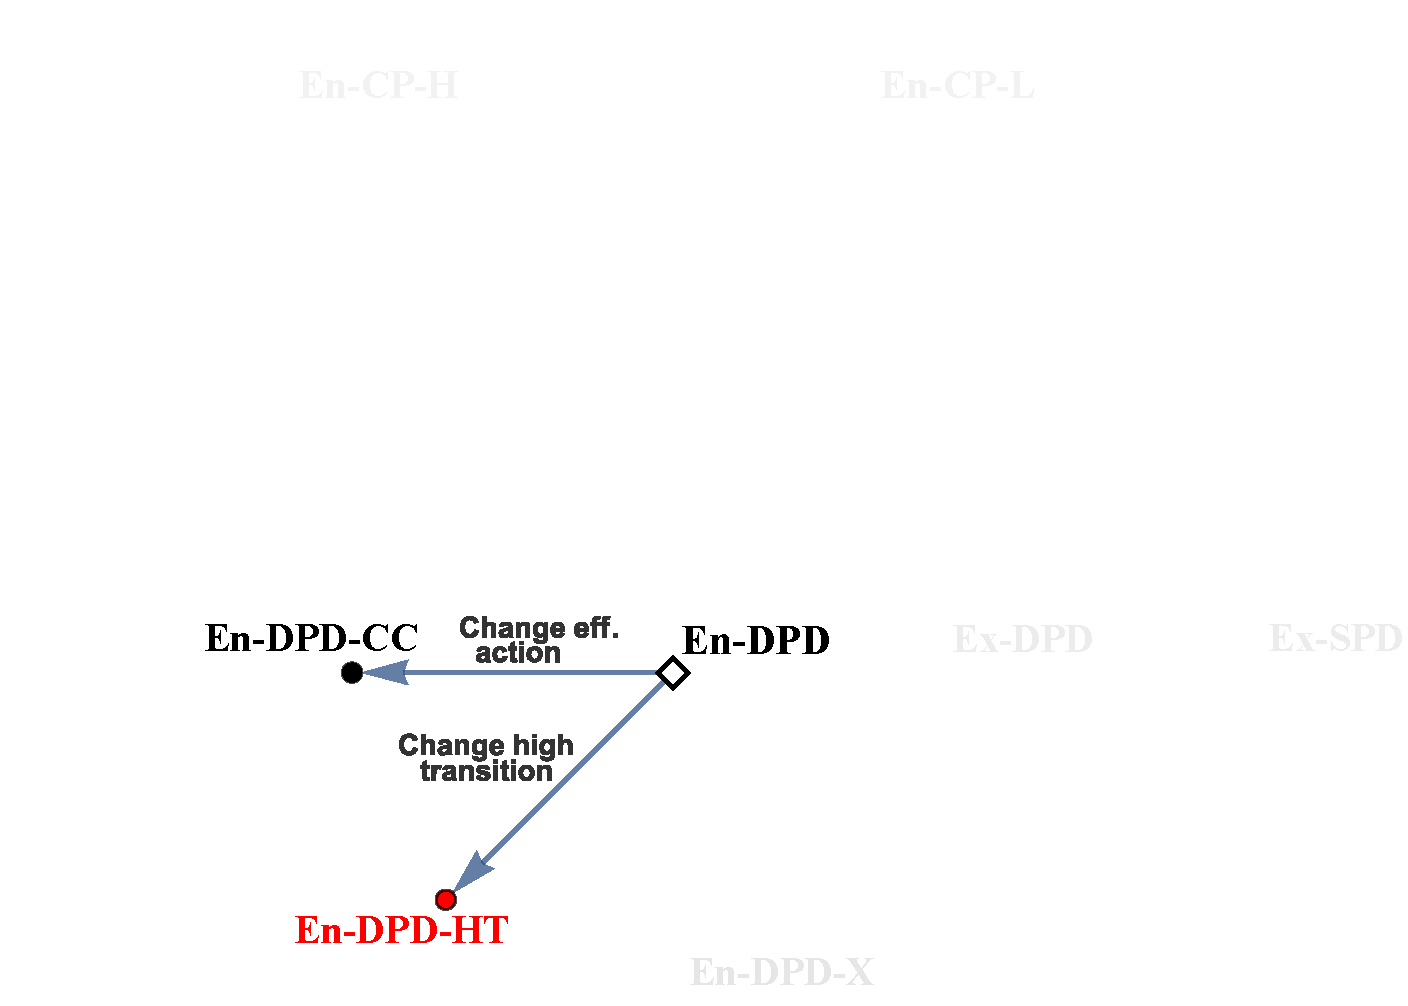
\includegraphics[height=0.7\textwidth]{../../../../p/vw_MPE/img/FlowChart3.pdf}
\end{center}
\end{frame}


\begin{frame}{En-DPD-2 $\rightarrow$ En-DPD-3}
\begin{itemize}
\item From En-DPD-2 (the pivot) only (D,D) in high causes Low next round
\item Subjects can unilaterally impose the high state once there
\item IR payoff is obtained by cooperating\pause
\item \textbf{Manipulation 2:} Change transition rule in high state

\begin{itemize}
\item Require joint cooperation to stay in High
\item (D,D), (C,D) and (D,C) in High lead to Low next round
\item Change IR payoff in High
\end{itemize}
\end{itemize}
\end{frame}

\begin{frame}{Endog-Dynamic-PD$\rightarrow$}

\begin{center}
\begin{table}
\centering{}\subfloat{\centering{}{\small{}}%
\begin{tabular}{cc>{\centering}p{0.1\textwidth}|>{\centering}p{0.1\textwidth}}
\multicolumn{4}{c}{\textcolor{red}{$\omega$=Low}}\tabularnewline
 &  & \multicolumn{1}{>{\centering}p{0.1\textwidth}}{} & \tabularnewline
 &  & \multicolumn{2}{c}{2}\tabularnewline
 &  & \multicolumn{1}{>{\centering}p{0.1\textwidth}}{\textbf{C}} & D\tabularnewline
\cline{3-4}
\multirow{2}{*}{1} & \multicolumn{1}{c|}{\textbf{C}} & \textcolor{blue}{100} & \multicolumn{1}{>{\centering}p{0.1\textwidth}|}{\textcolor{red}{30}}\tabularnewline
\cline{3-4}
 & \multicolumn{1}{c|}{D} & \textcolor{red}{125} & \multicolumn{1}{>{\centering}p{0.1\textwidth}|}{\textcolor{red}{60}}\tabularnewline
\cline{3-4}
\end{tabular}}\subfloat{\centering{}{\small{}}%
\begin{tabular}{cc>{\centering}p{0.1\textwidth}|>{\centering}p{0.1\textwidth}}
\multicolumn{4}{c}{\textcolor{blue}{$\omega$=High}}\tabularnewline
 &  & \multicolumn{1}{>{\centering}p{0.1\textwidth}}{} & \tabularnewline
 &  & \multicolumn{2}{c}{2}\tabularnewline
 &  & \multicolumn{1}{>{\centering}p{0.1\textwidth}}{C} & \textbf{D}\tabularnewline
\cline{3-4}
\multirow{2}{*}{1} & \multicolumn{1}{c|}{C} & \textcolor{blue}{200} & \multicolumn{1}{>{\centering}p{0.1\textwidth}|}{\textcolor{blue}{130}}\tabularnewline
\cline{3-4}
 & \multicolumn{1}{c|}{\textbf{D}} & \textcolor{blue}{280} & \multicolumn{1}{>{\centering}p{0.1\textwidth}|}{\textcolor{red}{190}}\tabularnewline
\cline{3-4}
\end{tabular}}
\end{table}

\par\end{center}

\begin{center}
\[
\psi\left(\mbox{\ensuremath{\omega}},a\right)=\begin{cases}
\mbox{High} & \mbox{if }a=\left(C,C\right),\mbox{\ensuremath{\omega}=Low}\\
\mbox{Low} & \mbox{if }a=\left(D,D\right),\mbox{\ensuremath{\omega}=High}\\
\omega & \mbox{otherwise}
\end{cases}
\]

\par\end{center}

$C-D$ unique MPE.

\end{frame}\begin{frame}{Endog-Dynamic-PD-2$\rightarrow$Endog-Dynamic-PD-HT}

\begin{center}
\begin{table}
\centering{}\subfloat{\centering{}{\small{}}%
\begin{tabular}{cc>{\centering}p{0.1\textwidth}|>{\centering}p{0.1\textwidth}}
\multicolumn{4}{c}{\textcolor{red}{$\omega$=Low}}\tabularnewline
 &  & \multicolumn{1}{>{\centering}p{0.1\textwidth}}{} & \tabularnewline
 &  & \multicolumn{2}{c}{2}\tabularnewline
 &  & \multicolumn{1}{>{\centering}p{0.1\textwidth}}{\textbf{C}} & D\tabularnewline
\cline{3-4}
\multirow{2}{*}{1} & \multicolumn{1}{c|}{\textbf{C}} & \textcolor{blue}{100} & \multicolumn{1}{>{\centering}p{0.1\textwidth}|}{\textcolor{red}{30}}\tabularnewline
\cline{3-4}
 & \multicolumn{1}{c|}{D} & \textcolor{red}{125} & \multicolumn{1}{>{\centering}p{0.1\textwidth}|}{\textcolor{red}{60}}\tabularnewline
\cline{3-4}
\end{tabular}}\subfloat{\centering{}{\small{}}%
\begin{tabular}{cc>{\centering}p{0.1\textwidth}|>{\centering}p{0.1\textwidth}}
\multicolumn{4}{c}{\textcolor{blue}{$\omega$=High}}\tabularnewline
 &  & \multicolumn{1}{>{\centering}p{0.1\textwidth}}{} & \tabularnewline
 &  & \multicolumn{2}{c}{2}\tabularnewline
 &  & \multicolumn{1}{>{\centering}p{0.1\textwidth}}{C} & \textbf{D}\tabularnewline
\cline{3-4}
\multirow{2}{*}{1} & \multicolumn{1}{c|}{C} & \textcolor{blue}{200} & \multicolumn{1}{>{\centering}p{0.1\textwidth}|}{\textcolor{red}{130}}\tabularnewline
\cline{3-4}
 & \multicolumn{1}{c|}{\textbf{D}} & \textcolor{red}{280} & \multicolumn{1}{>{\centering}p{0.1\textwidth}|}{\textcolor{red}{190}}\tabularnewline
\cline{3-4}
\end{tabular}}
\end{table}

\par\end{center}

\begin{center}
\[
\psi\left(\mbox{\ensuremath{\omega}},a\right)=\begin{cases}
\mbox{High} & \mbox{if }a=\left(C,C\right)\\
\mbox{Low} & \mbox{otherwise.}
\end{cases}
\]

\par\end{center}
\begin{itemize}
\item $C-D$ still MPE, but $D-D$ now also
\item $D-C$ is an MPE, but starting state is \emph{Low}
\end{itemize}
\end{frame}\begin{frame}{Results: Cooperation by State}

\begin{center}
	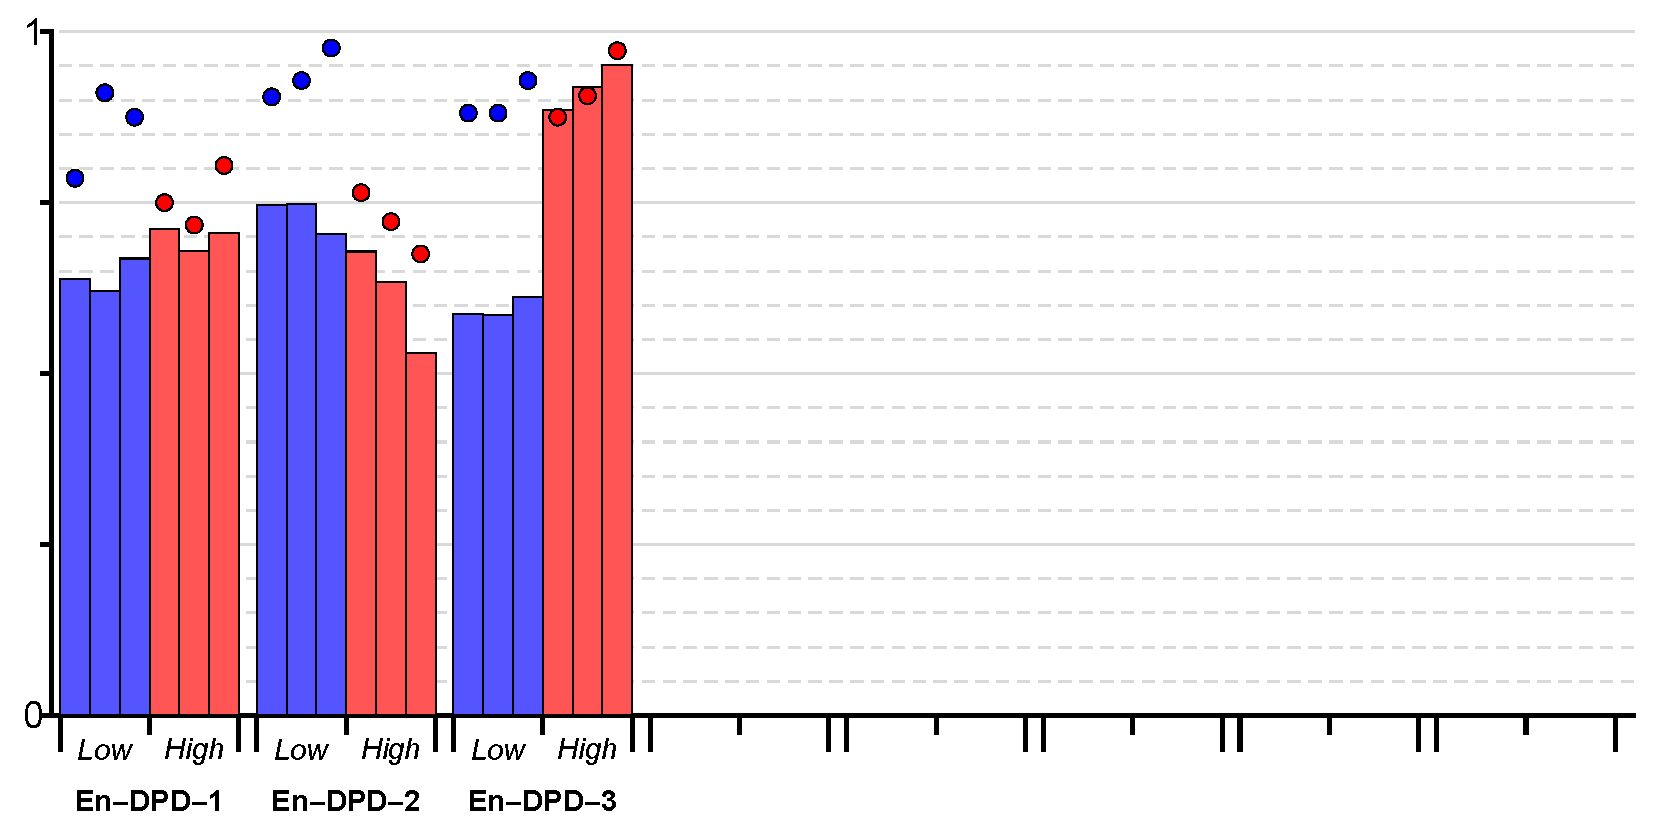
\includegraphics[width=1.0\textwidth]{../../../../p/vw_MPE/img/col_bar_StateCoop_block_EnDPD_H.pdf}
\end{center}

{
\small \begin{itemize}\item Points indicate Cooperation rate in first/second round for low/high state
\item Blocks of cycles 1--5, 6--10, 11--15
\end{itemize}
}\end{frame}
\begin{frame}{Subject Cooperation:En-DPD$\rightarrow$\only<2>{En-DPD-HT} }


\begin{center}
	\includegraphics<1>[width=0.6\textwidth]{../../../../p/vw_MPE/img/col_subject_stateCooperation_L5_EnDPD_2.pdf}
	\includegraphics<2>[width=0.6\textwidth]{../../../../p/vw_MPE/img/col_subject_stateCooperation_L5_EnDPD_H.pdf}
\end{center}

\end{frame}

% \begin{frame}{Sequences}

% \begin{itemize}
% \item Five most popular sequences across rounds 1--5 are:

% \begin{itemize}
% \item \textcolor{red}{CC},\textcolor{blue}{CC},\textcolor{blue}{CC},\textcolor{blue}{CC},\textcolor{blue}{CC}
% (58\% of cycles)
% \item \textcolor{red}{CC},\textcolor{blue}{CC},\textcolor{blue}{CC},\textcolor{blue}{CC},\textcolor{blue}{DC}
% (12\% of cycles)
% \item \textcolor{red}{CC},\textcolor{blue}{CC},\textcolor{blue}{CC},\textcolor{blue}{DC},\textcolor{red}{DC}
% (3\% of cycles)
% \end{itemize}
% \item Looks very cooperative

% \begin{itemize}
% \item 73\% of cycles stay in High state in periods 2--5
% \item Only 3\% of cycles alternate Low, High, Low, ...
% \item 6\% of cycles never reach High state.
% \end{itemize}
% \end{itemize}
% \end{frame}

\begin{frame}{Strategies (En-DPD$\rightarrow$En-DPD-HT)}

\begin{itemize}
\item Popular pure strategy Markov:

\begin{itemize}
\item C-C: $7.9\%\rightarrow24.5\%$
\item C-D: $23.5\%\rightarrow2.0\%$
\item D-D: $4.7\%\rightarrow2.4\%$
\end{itemize}
\item Popular history-dependent strategies

\begin{itemize}
\item Grim trigger $13.8\%\rightarrow34.0\%$
\end{itemize}
\item \textbf{Strategies highly cooperative, but much less forgiving}
\item \textbf{Very little MPE play or MPE triggers}
\end{itemize}
\end{frame}

% \begin{frame}{Subject-level Response}

% \begin{itemize}
% \item Subject in Ex-DPD: \only<1>{Subject Always-C?}
% \only<2>{Subject Grim trigger}
% \end{itemize}

% \begin{center}
% \includegraphics<1>[height=0.5\textheight]{../../../../p/vw_MPE/img/subject/EnDPD_H21.pdf}
% \includegraphics<2>[height=0.5\textheight]{../../../../p/vw_MPE/img/subject/EnDPD_H23.pdf}
% \end{center}


% \end{frame}

\begin{frame}


\textbf{Result 3: }



\textbf{Reducing the IR payoff increases cooperation, punishments
used are harsher}
\end{frame}

\begin{frame}


\begin{center}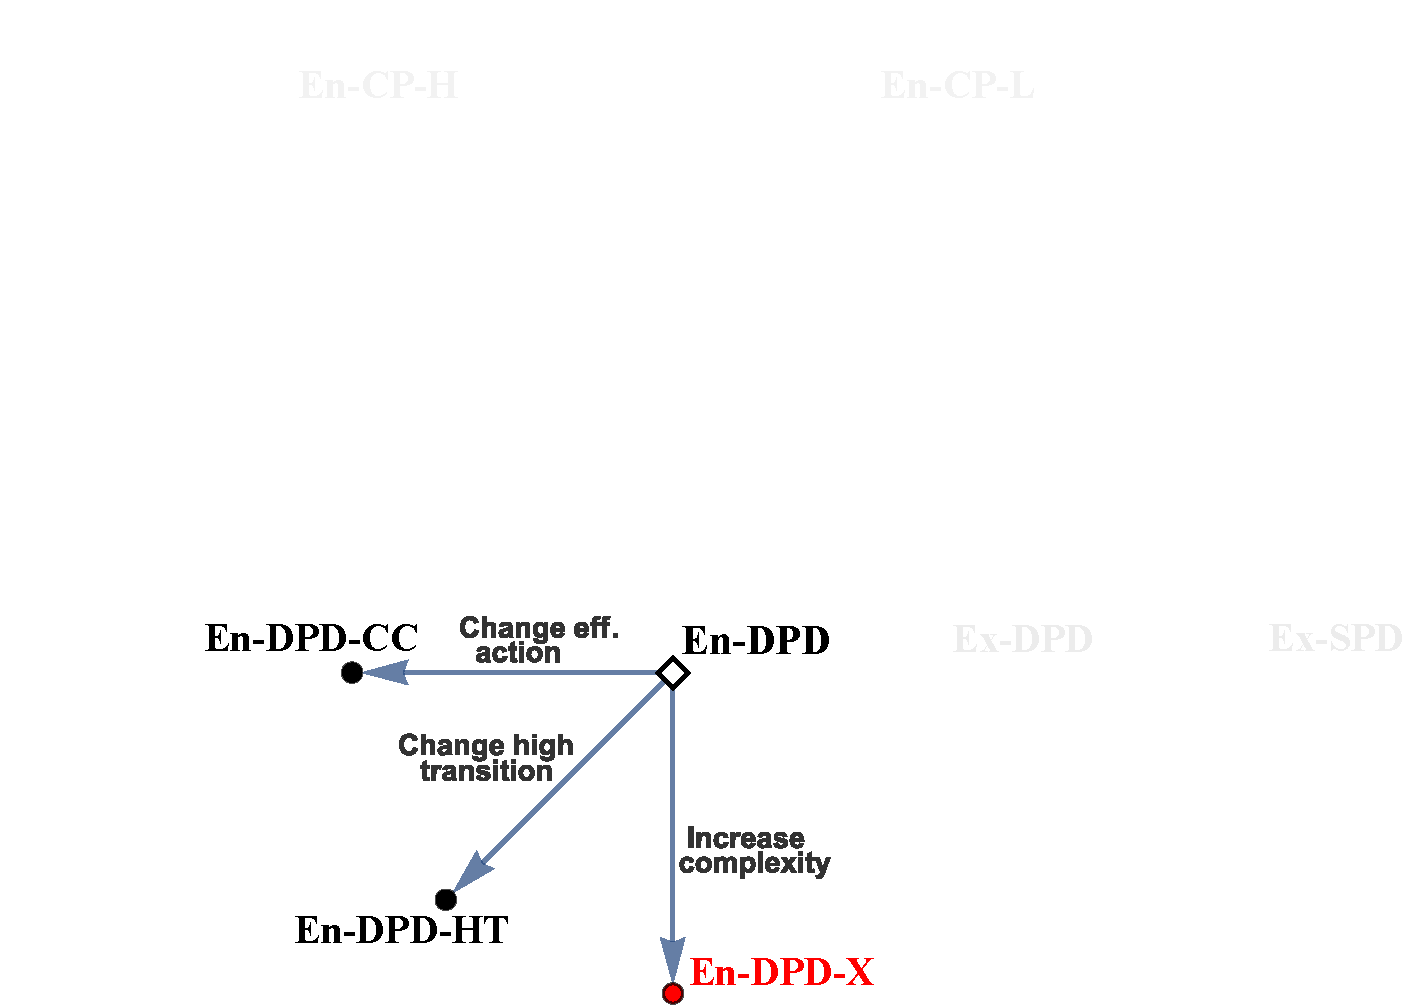
\includegraphics[height=0.7\textwidth]{../../../../p/vw_MPE/img/FlowChart4.pdf}
\end{center}
\end{frame}


\begin{frame}{En-DPD $\rightarrow$ En-DPD-X}
\begin{itemize}
\item Computational complexity literature identifies complexity as one reason
to select MPE
\item One measure of complexity is the number of payoff relevant states

\begin{itemize}
\item Our En-DPD games only have 2 states...
\end{itemize}
\item Does making the game more complex leads to more Markov play?\pause
\item \textbf{Manipulation 3:} Make the game more complex

\begin{itemize}
\item Same game as En-DPD with added exogenous shocks each round
\item Draw a number $x$ uniformly over $X=\left\{ -5,-4,\ldots,4,5\right\} $
\item State space is now $\left\{ \mbox{Low},\mbox{High}\right\} \times X$
\item 2 states $\rightarrow$ 22 states.
\end{itemize}
\end{itemize}
\end{frame}
\begin{frame}{Complex Endog-Dynamic-PD-2}


\begin{center}
\begin{table}
\centering{}\subfloat{\centering{}{\small{}}%
\begin{tabular}{cc>{\centering}p{0.1\textwidth}|>{\centering}p{0.1\textwidth}}
\multicolumn{4}{c}{\textcolor{red}{$\omega$=Low}}\tabularnewline
 &  & \multicolumn{1}{>{\centering}p{0.1\textwidth}}{} & \tabularnewline
 &  & \multicolumn{2}{c}{2}\tabularnewline
 &  & \multicolumn{1}{>{\centering}p{0.1\textwidth}}{\textbf{C}} & D\tabularnewline
\cline{3-4}
\multirow{2}{*}{1} & \multicolumn{1}{c|}{\textbf{C}} & \textcolor{blue}{100+x} & \multicolumn{1}{>{\centering}p{0.1\textwidth}|}{\textcolor{red}{30+x}}\tabularnewline
\cline{3-4}
 & \multicolumn{1}{c|}{D} & \textcolor{red}{125-x} & \multicolumn{1}{>{\centering}p{0.1\textwidth}|}{\textcolor{red}{60-x}}\tabularnewline
\cline{3-4}
\end{tabular}}\subfloat{\centering{}{\small{}}%
\begin{tabular}{cc>{\centering}p{0.12\textwidth}|>{\centering}p{0.12\textwidth}}
\multicolumn{4}{c}{\textcolor{blue}{$\omega$=High}}\tabularnewline
 &  & \multicolumn{1}{>{\centering}p{0.12\textwidth}}{} & \tabularnewline
 &  & \multicolumn{2}{c}{2}\tabularnewline
 &  & \multicolumn{1}{>{\centering}p{0.12\textwidth}}{C} & \textbf{D}\tabularnewline
\cline{3-4}
\multirow{2}{*}{1} & \multicolumn{1}{c|}{C} & \textcolor{blue}{200+2x} & \multicolumn{1}{>{\centering}p{0.12\textwidth}|}{\textcolor{blue}{130+2x}}\tabularnewline
\cline{3-4}
 & \multicolumn{1}{c|}{\textbf{D}} & \textcolor{blue}{280-2x} & \multicolumn{1}{>{\centering}p{0.12\textwidth}|}{\textbf{\textcolor{red}{190-2x}}}\tabularnewline
\cline{3-4}
\end{tabular}}
\end{table}

\par\end{center}


\textrm{
\[
\psi\left(\mbox{\ensuremath{\omega}},a\right)=\begin{cases}
\left(\mbox{High},y\right) & \mbox{if }a=\left(C,C\right),\omega=\left(\mbox{Low},x\right)\\
\left(\mbox{Low},y\right) & \mbox{if }a=\left(D,D\right),\omega=\left(\mbox{High},x\right)\\
\left(\omega_{1},y\right) & \mbox{otherwise}
\end{cases}
\]
}
\begin{itemize}
\item $y\perp x$, uniformly distributed on $\left\{ -5,-4,\ldots,4,5\right\} $
\item $C-D$ in \emph{Low/High} and ignoring $x$ an MPE (not unique though)
\end{itemize}
\end{frame}


\begin{frame}{Results: Cooperation by State}

\begin{center}
	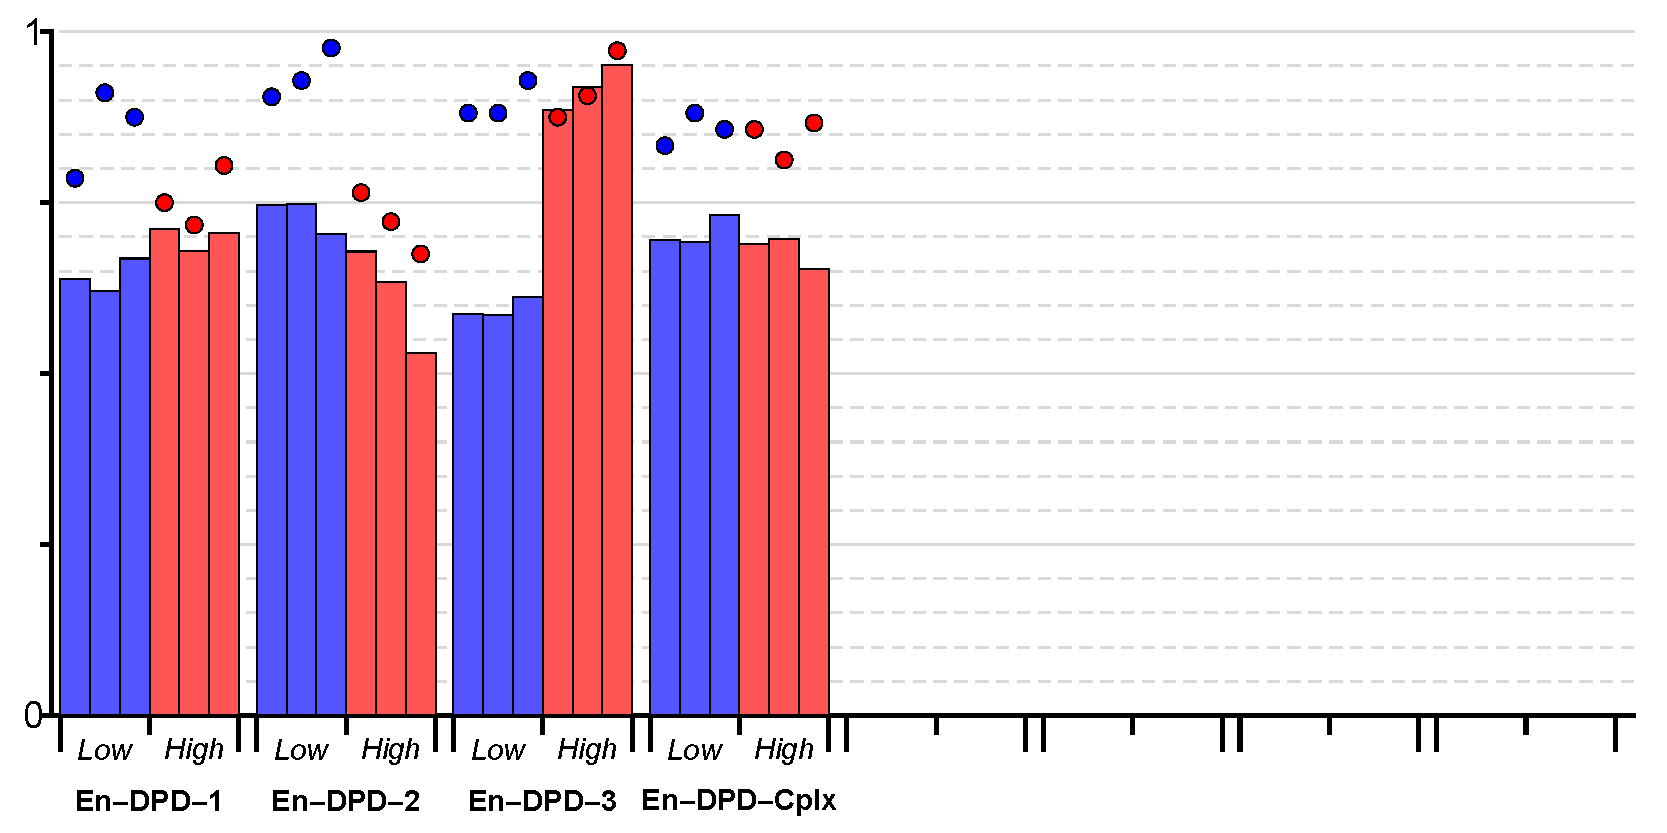
\includegraphics[width=1.0\textwidth]{../../../../p/vw_MPE/img/col_bar_StateCoop_block_EnDPD_C.pdf}
\end{center}

{\small \begin{itemize}\item Points indicate Cooperation rate in first/second round for low/high state
\item Blocks of cycles 1--5, 6--10, 11--15
\end{itemize}
}\end{frame}
\begin{frame}{Subject Cooperation: En-DPD$\rightarrow$\only<2>{En-DPD-X} }


\begin{center}
	\includegraphics<1>[width=0.6\textwidth]{../../../../p/vw_MPE/img/col_subject_stateCooperation_L5_EnDPD_2.pdf}
	\includegraphics<2>[width=0.6\textwidth]{../../../../p/vw_MPE/img/col_subject_stateCooperation_L5_EnDPD_C.pdf}
\end{center}

\end{frame}


\begin{frame}{Strategies (En-DPD$\rightarrow$En-DPD-X)}
\begin{itemize}
\item Markov strategies (ignoring small-shocks)

\begin{itemize}
\item C-C: $7.9\%\rightarrow31.4\%$
\item \textbf{C-D:} $23.5\%\rightarrow19.1\%$
\item D-D\textbf{:} $4.7\%\rightarrow2.7\%$
\end{itemize}
\item Popular history-dependent strategies

\begin{itemize}
\item MPE-trigger $7.8\%\rightarrow19.0\%$
\item C-Alternate, MPE-trigger $23.4\%\rightarrow14.2\%$
\end{itemize}
\item \textbf{Despite added complexity, subjects react similarly to En-DPD-2}
\item Small perturbations to game structure yield similar behavior
\end{itemize}
\end{frame}
\begin{frame}


\textbf{Result 4: }



\textbf{Small changes to the games payoffs lead to small deviations
in behavior even with much increased complexity. Increased complexity
does not lead to increased selection of MPE.}
\end{frame}


\begin{frame}{Dynamic PD game summary}
\begin{itemize}
\item Across a series of manipulations to a similar Dynamic PD game we find
effects over

\begin{itemize}
\item where conditional cooperation is targeted
\item the types of punishments that support it
\end{itemize}
\item But little differences in rate of MPE selection
\item Let's make larger changes in the structure of the game
\end{itemize}
\end{frame}
\begin{frame}


\begin{center}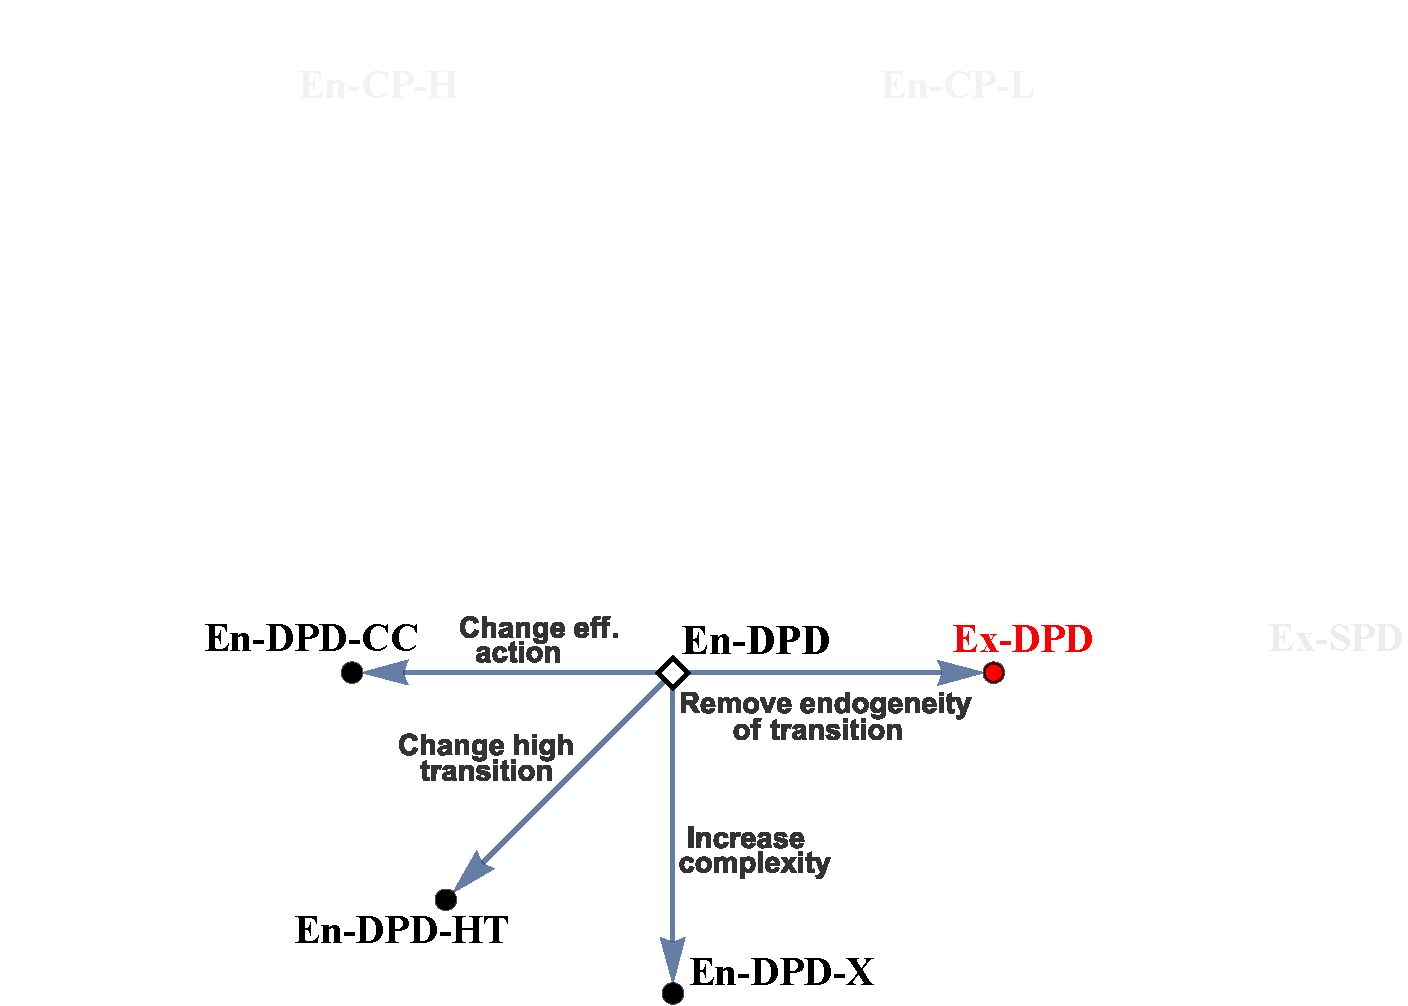
\includegraphics[height=0.7\textwidth]{../../../../p/vw_MPE/img/FlowChart5.pdf}
\end{center}
\end{frame}


\begin{frame}{En-DPD-2 $\rightarrow$ Ex-DPD-2}
\begin{itemize}
\item In the En-DPD games the transitions are endogenous, so there is a
dynamic externality

\begin{itemize}
\item My actions affect the state, which affects the other player's payoff
\end{itemize}
\item What are the effects of removing the dynamic externality?\pause
\item \textbf{Manipulation 4:} Eliminate the dynamic externality

\begin{itemize}
\item Exogenous random transition between states
\item Choose probabilities to match observed state frequency in En-DPD
\item Hold game payoffs constant
\end{itemize}
\end{itemize}
\end{frame}

\begin{frame}{Endog-Dynamic-PD}

\begin{center}
\begin{table}
\centering{}\subfloat{\centering{}{\small{}}%
\begin{tabular}{cc>{\centering}p{0.1\textwidth}|>{\centering}p{0.1\textwidth}}
\multicolumn{4}{c}{\textcolor{red}{$\omega$=Low}}\tabularnewline
 &  & \multicolumn{1}{>{\centering}p{0.1\textwidth}}{} & \tabularnewline
 &  & \multicolumn{2}{c}{2}\tabularnewline
 &  & \multicolumn{1}{>{\centering}p{0.1\textwidth}}{\textbf{C}} & D\tabularnewline
\cline{3-4}
\multirow{2}{*}{1} & \multicolumn{1}{c|}{\textbf{C}} & \textcolor{blue}{100} & \multicolumn{1}{>{\centering}p{0.1\textwidth}|}{\textcolor{red}{30}}\tabularnewline
\cline{3-4}
 & \multicolumn{1}{c|}{D} & \textcolor{red}{125} & \multicolumn{1}{>{\centering}p{0.1\textwidth}|}{\textcolor{red}{60}}\tabularnewline
\cline{3-4}
\end{tabular}}\subfloat{\centering{}{\small{}}%
\begin{tabular}{cc>{\centering}p{0.1\textwidth}|>{\centering}p{0.1\textwidth}}
\multicolumn{4}{c}{\textcolor{blue}{$\omega$=High}}\tabularnewline
 &  & \multicolumn{1}{>{\centering}p{0.1\textwidth}}{} & \tabularnewline
 &  & \multicolumn{2}{c}{2}\tabularnewline
 &  & \multicolumn{1}{>{\centering}p{0.1\textwidth}}{C} & \textbf{D}\tabularnewline
\cline{3-4}
\multirow{2}{*}{1} & \multicolumn{1}{c|}{C} & \textcolor{blue}{200} & \multicolumn{1}{>{\centering}p{0.1\textwidth}|}{\textcolor{blue}{130}}\tabularnewline
\cline{3-4}
 & \multicolumn{1}{c|}{\textbf{D}} & \textcolor{blue}{280} & \multicolumn{1}{>{\centering}p{0.1\textwidth}|}{\textbf{\textcolor{red}{190}}}\tabularnewline
\cline{3-4}
\end{tabular}}
\end{table}

\par\end{center}

\textrm{
\[
\psi\left(\mbox{\ensuremath{\omega}},a\right)=\begin{cases}
\mbox{High} & \mbox{if }a=\left(C,C\right),\mbox{\ensuremath{\omega}=Low}\\
\mbox{Low} & \mbox{if }a=\left(D,D\right),\mbox{\ensuremath{\omega}=High}\\
\omega & \mbox{otherwise}
\end{cases}
\]
}

Unique MPE is C-D

\end{frame}\begin{frame}{Exog-Dynamic-PD}

\begin{table}
\centering{}\subfloat{\centering{}{\small{}}%
\begin{tabular}{cc>{\centering}p{0.1\textwidth}|>{\centering}p{0.1\textwidth}}
\multicolumn{4}{c}{\textcolor{red}{$\omega$=Low}}\tabularnewline
 &  & \multicolumn{1}{>{\centering}p{0.1\textwidth}}{} & \tabularnewline
 &  & \multicolumn{2}{c}{2}\tabularnewline
 &  & \multicolumn{1}{>{\centering}p{0.1\textwidth}}{\textbf{C}} & D\tabularnewline
\cline{3-4}
\multirow{2}{*}{1} & \multicolumn{1}{c|}{\textbf{C}} & \textcolor{black}{100} & \multicolumn{1}{>{\centering}p{0.1\textwidth}|}{\textcolor{black}{30}}\tabularnewline
\cline{3-4}
 & \multicolumn{1}{c|}{D} & \textcolor{black}{125} & \multicolumn{1}{>{\centering}p{0.1\textwidth}|}{\textcolor{black}{60}}\tabularnewline
\cline{3-4}
\end{tabular}}\subfloat{\centering{}{\small{}}%
\begin{tabular}{cc>{\centering}p{0.1\textwidth}|>{\centering}p{0.1\textwidth}}
\multicolumn{4}{c}{\textcolor{blue}{$\omega$=High}}\tabularnewline
 &  & \multicolumn{1}{>{\centering}p{0.1\textwidth}}{} & \tabularnewline
 &  & \multicolumn{2}{c}{2}\tabularnewline
 &  & \multicolumn{1}{>{\centering}p{0.1\textwidth}}{C} & \textbf{D}\tabularnewline
\cline{3-4}
\multirow{2}{*}{1} & \multicolumn{1}{c|}{C} & \textcolor{black}{200} & \multicolumn{1}{>{\centering}p{0.1\textwidth}|}{\textcolor{black}{130}}\tabularnewline
\cline{3-4}
 & \multicolumn{1}{c|}{\textbf{D}} & \textcolor{black}{280} & \multicolumn{1}{>{\centering}p{0.1\textwidth}|}{\textbf{\textcolor{black}{190}}}\tabularnewline
\cline{3-4}
\end{tabular}}
\end{table}


\textrm{
\[
\psi\left(\mbox{\ensuremath{\omega}},a\right)=\begin{cases}
0.6\cdot\mbox{High}\oplus0.4\cdot\mbox{Low} & \mbox{if \ensuremath{\omega}=Low}\\
0.8\cdot\mbox{High}\oplus0.2\cdot\mbox{Low} & \mbox{if }\mbox{\ensuremath{\omega}=High}
\end{cases}
\]
}

Unique MPE now $D-D$, but efficient SPE still possible!

\end{frame}

\begin{frame}{Results: Cooperation by State}

\begin{center}
	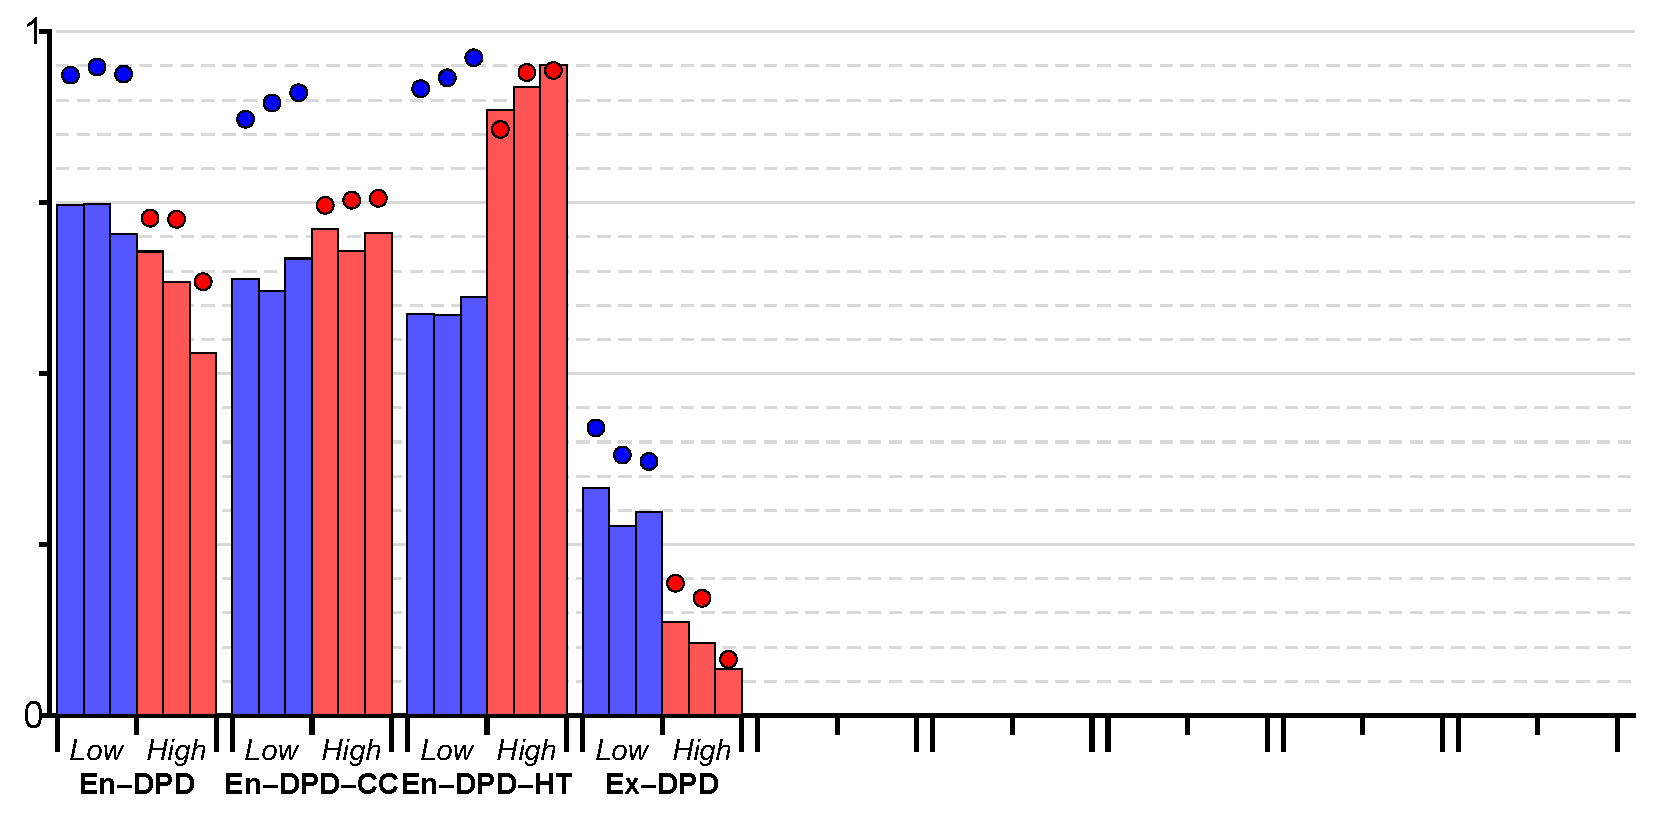
\includegraphics[width=1.0\textwidth]{../../../../p/vw_MPE/img/col_bar_StateCoop_block_ExDPD.pdf}
\end{center}

{\small \begin{itemize}\item Points indicate Cooperation rate in first/second round for low/high state
\item Blocks of cycles 1--5, 6--10, 11--15
\end{itemize}
}\end{frame}
\begin{frame}{Subject Cooperation:En-DPD$\rightarrow$\only<2>{Ex-DPD} }


\begin{center}
	\includegraphics<1>[width=0.6\textwidth]{../../../../p/vw_MPE/img/col_subject_stateCooperation_L5_EnDPD_2.pdf}
	\includegraphics<2>[width=0.6\textwidth]{../../../../p/vw_MPE/img/col_subject_stateCooperation_L5_ExDPD.pdf}
\end{center}

\end{frame}

\begin{frame}{Sequences}

\begin{itemize}
\item Five most popular sequences across rounds 1--5 are:

\begin{itemize}
\item DD,DD,DD,DD,DD (39\% of cycles)
\item DC,DD,DD,DD,DD (35\%)
\item CC,CC,DC,DD,DD (4\%)
\end{itemize}
\item Mostly defections, or failed attempt at cooperation
\end{itemize}
\end{frame}

\begin{frame}{Strategies (En-DPD$\rightarrow$Ex-DPD)}

\begin{itemize}
\item Popular pure strategy Markov:

\begin{itemize}
\item C-C: $7.9\%\rightarrow0.0\%$
\item C-D: $23.5\%\rightarrow7.3\%$
\item D-D (MPE): $4.7\%\rightarrow63.2\%$
\end{itemize}
\item Popular history-dependent strategies

\begin{itemize}
\item Grim trigger $13.8\%\rightarrow19.5\%$
\end{itemize}
\item \textbf{Most attempts at cooperation are in low state; majority defect
in all states}
\end{itemize}
\end{frame}

\begin{frame}


\textbf{Result 5: }



\textbf{Without the dynamic externality subjects cooperation falls
markedly}
\end{frame}

\begin{frame}


\begin{center}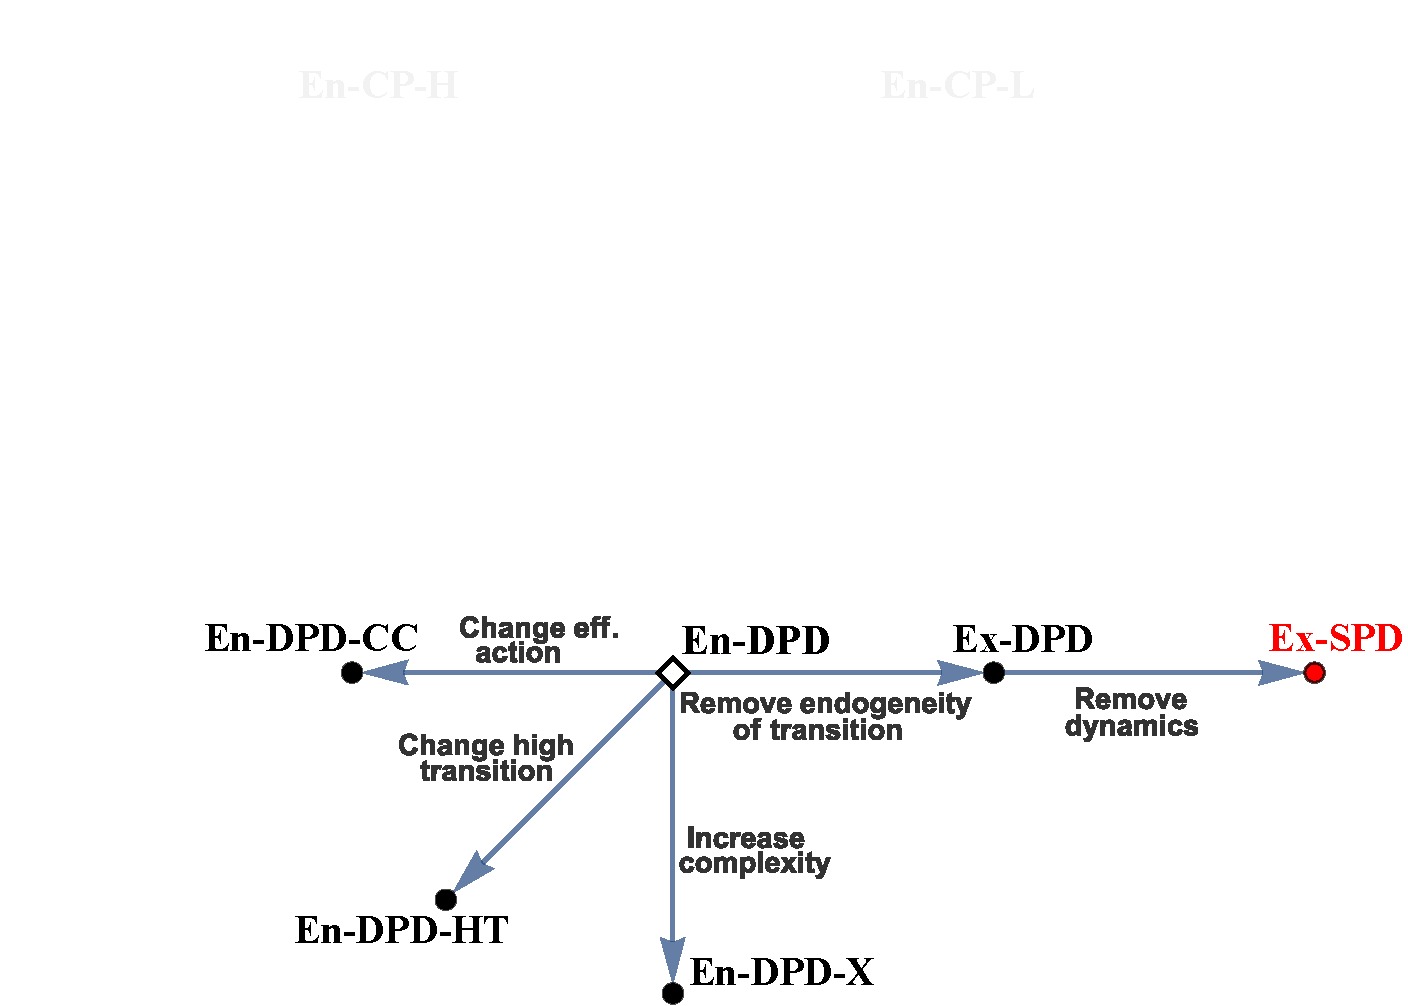
\includegraphics[height=0.7\textwidth]{../../../../p/vw_MPE/img/FlowChart6.pdf}
\end{center}
\end{frame}


\begin{frame}{En/Ex-DPD-2 $\rightarrow$ Ex-SPD-2}
\begin{itemize}
\item In our Dynamic-PD games, the state is changing over time
\item What is the effect in the Exog-DPD from the changing state?

\begin{itemize}
\item What are the cooperation levels in each repeated game separately?\pause
\end{itemize}
\item \textbf{Manipulation 5:} Remove dynamics within cycles:

\begin{itemize}
\item At the start of the game, randomly select either High or Low
\item State tomorrow equals state today.
\item Each cycle is an indefinitely repeated PD game
\end{itemize}
\end{itemize}
\end{frame}

\begin{frame}{Results: Cooperation by State}

\begin{center}
	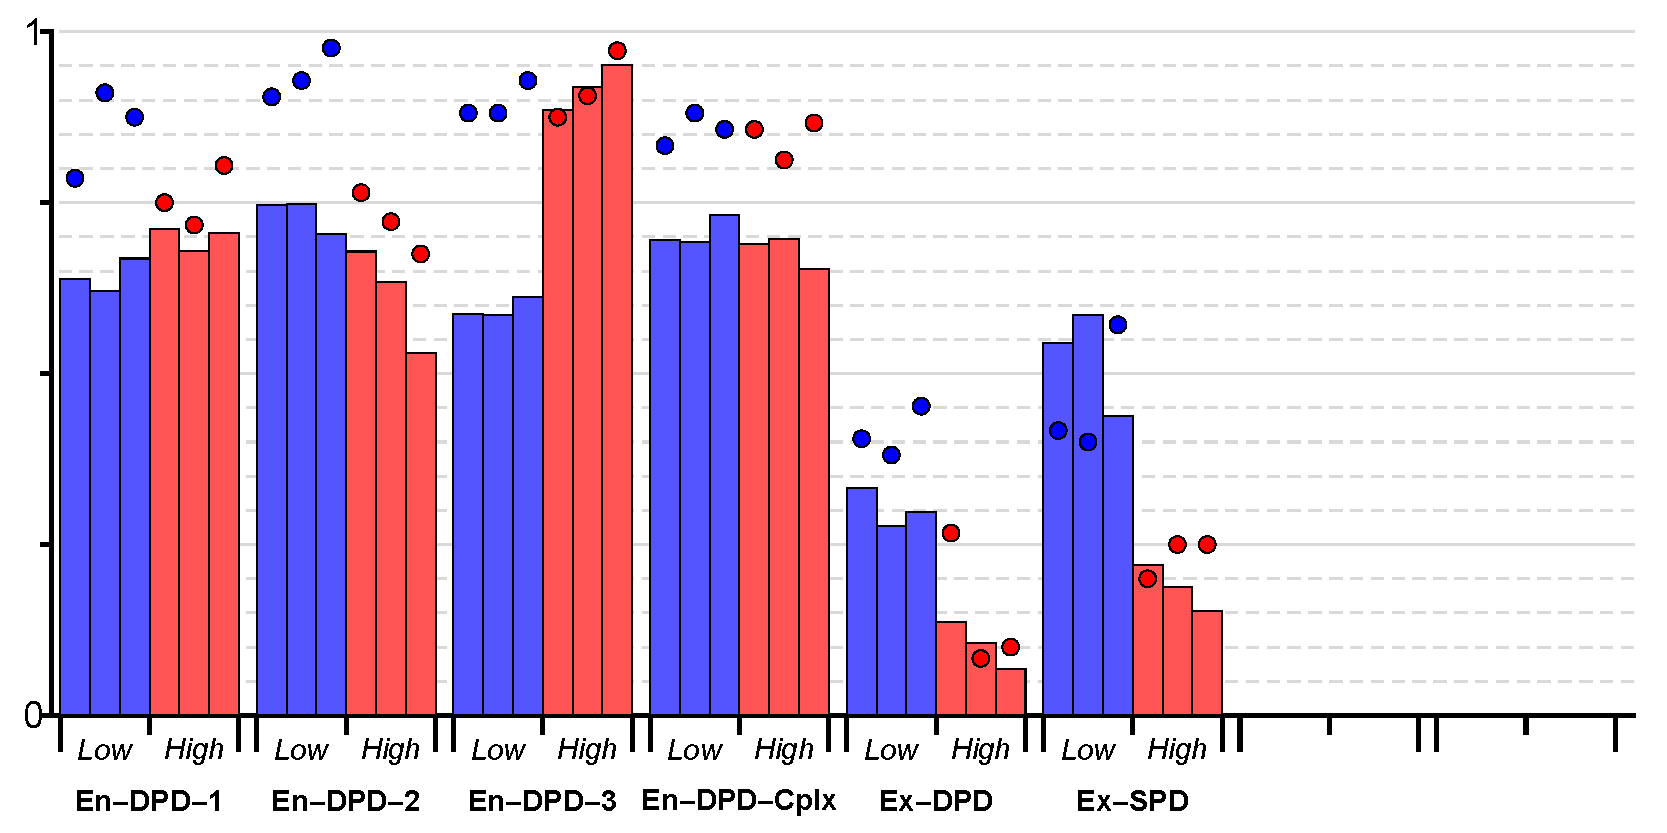
\includegraphics[width=1.0\textwidth]{../../../../p/vw_MPE/img/col_bar_StateCoop_block_ExIRPD.pdf}
\end{center}

{\small \begin{itemize}\item Points indicate Cooperation rate in first/second round for low/high state
\item Blocks of cycles 1--5, 6--10, 11--15
\end{itemize}
}\end{frame}
\begin{frame}{Subject Cooperation:Ex-DPD$\rightarrow$\only<2>{Ex-SPD} }


\begin{center}
	\includegraphics<1>[width=0.6\textwidth]{../../../../p/vw_MPE/img/col_subject_stateCooperation_L5_ExDPD.pdf}
	\includegraphics<2>[width=0.6\textwidth]{../../../../p/vw_MPE/img/col_subject_stateCooperation_L5_ExIRPD.pdf}
\end{center}

\end{frame}

\begin{frame}{Strategies (Ex/En-DPD$\rightarrow$SPD)}

\begin{itemize}
\item Cooperation rates at each state match behavior in each game:

\begin{itemize}
\item Low state, Grim is risk-dominant, observe more cooperation
\item High state, All-D is risk dominant, observe mostly defections
\end{itemize}
\item \textbf{Removing the dynamics increases cooperation in the low state}
\end{itemize}
\end{frame}

\begin{frame}


\textbf{Result 6: }



\textbf{Dynamically evolving (but exogenous) environments reduce conditional
cooperation}
\end{frame}

\begin{frame}


\begin{center}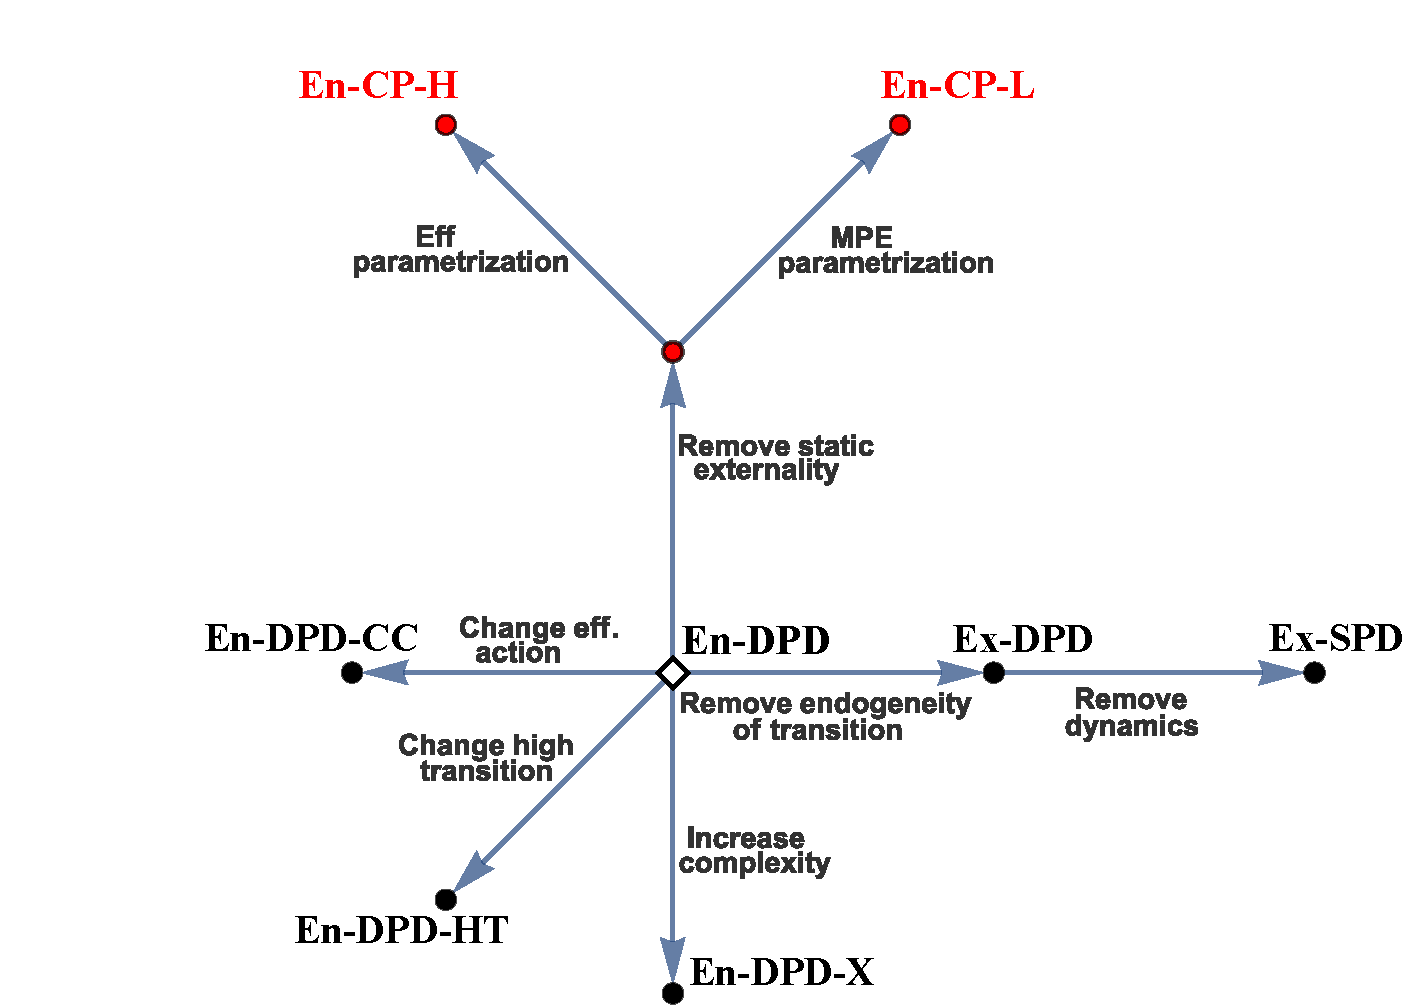
\includegraphics[height=0.7\textwidth]{../../../../p/vw_MPE/img/FlowChart7.pdf}
\end{center}
\end{frame}


\begin{frame}{En-DPD$\rightarrow$ En-CP}
\begin{itemize}
\item In PD games, the action choice today has a static externality, my
action choice affects your payoff today
\item We know that removing the dynamic externality reduces cooperation,
but what are the effects from removing the static externality?\pause
\item \textbf{Manipulation 6 \& 7:} Remove the static externalities:

\begin{itemize}
\item Same transition rule as En-DPD
\item Player 1's payoff today unaffected by Player 2's action today
\item Two parametrizations:

\begin{itemize}
\item One has same MPE tensions as En-DPD
\item One has same efficient frontier as En-DPD
\end{itemize}
\end{itemize}
\end{itemize}
\end{frame}
\begin{frame}{Common Pool-Low}


\begin{center}
\begin{table}
\centering{}\subfloat{\centering{}{\small{}}%
\begin{tabular}{cc>{\centering}p{0.1\textwidth}|>{\centering}p{0.1\textwidth}}
\multicolumn{4}{c}{\textcolor{red}{$\omega$=Low}}\tabularnewline
 &  & \multicolumn{1}{>{\centering}p{0.1\textwidth}}{} & \tabularnewline
 &  & \multicolumn{2}{c}{2}\tabularnewline
 &  & \multicolumn{1}{>{\centering}p{0.1\textwidth}}{\textbf{C}} & D\tabularnewline
\cline{3-4}
\multirow{2}{*}{1} & \multicolumn{1}{c|}{\textbf{C}} & \textbf{\textcolor{blue}{100}} & \multicolumn{1}{>{\centering}p{0.1\textwidth}|}{\textcolor{red}{100}}\tabularnewline
\cline{3-4}
 & \multicolumn{1}{c|}{D} & \textcolor{red}{125} & \multicolumn{1}{>{\centering}p{0.1\textwidth}|}{\textcolor{red}{125}}\tabularnewline
\cline{3-4}
\end{tabular}}\subfloat{\centering{}{\small{}}%
\begin{tabular}{cc>{\centering}p{0.1\textwidth}|>{\centering}p{0.1\textwidth}}
\multicolumn{4}{c}{\textcolor{blue}{$\omega$=High}}\tabularnewline
 &  & \multicolumn{1}{>{\centering}p{0.1\textwidth}}{} & \tabularnewline
 &  & \multicolumn{2}{c}{2}\tabularnewline
 &  & \multicolumn{1}{>{\centering}p{0.1\textwidth}}{C} & \textbf{D}\tabularnewline
\cline{3-4}
\multirow{2}{*}{1} & \multicolumn{1}{c|}{C} & \textcolor{blue}{130} & \multicolumn{1}{>{\centering}p{0.1\textwidth}|}{\textcolor{blue}{130}}\tabularnewline
\cline{3-4}
 & \multicolumn{1}{c|}{\textbf{D}} & \textcolor{blue}{190} & \multicolumn{1}{>{\centering}p{0.1\textwidth}|}{\textbf{\textcolor{red}{190}}}\tabularnewline
\cline{3-4}
\end{tabular}}
\end{table}

\par\end{center}
\begin{itemize}
\item Same state transition rule as En-DPD, same symmetric Markov
\item Removes contemporaneous externality
\item Same tensions as the DPD game at the efficient MPE
\item Same MPE as En-DPD, $C$ in Low, $D$ in High (\textbf{$D$} in both
also)
\end{itemize}
\end{frame}

\begin{frame}{Common Pool-High}


\begin{center}
\begin{table}
\centering{}\subfloat{\centering{}{\small{}}%
\begin{tabular}{cc>{\centering}p{0.1\textwidth}|>{\centering}p{0.1\textwidth}}
\multicolumn{4}{c}{\textcolor{red}{$\omega$=Low}}\tabularnewline
 &  & \multicolumn{1}{>{\centering}p{0.1\textwidth}}{} & \tabularnewline
 &  & \multicolumn{2}{c}{2}\tabularnewline
 &  & \multicolumn{1}{>{\centering}p{0.1\textwidth}}{\textbf{C}} & D\tabularnewline
\cline{3-4}
\multirow{2}{*}{1} & \multicolumn{1}{c|}{\textbf{C}} & \textcolor{blue}{100} & \multicolumn{1}{>{\centering}p{0.1\textwidth}|}{\textcolor{red}{100}}\tabularnewline
\cline{3-4}
 & \multicolumn{1}{c|}{D} & \textcolor{red}{125} & \multicolumn{1}{>{\centering}p{0.1\textwidth}|}{\textcolor{red}{125}}\tabularnewline
\cline{3-4}
\end{tabular}}\subfloat{\centering{}{\small{}}%
\begin{tabular}{rc>{\centering}p{0.1\textwidth}|>{\centering}p{0.1\textwidth}}
\multicolumn{4}{c}{\textcolor{blue}{$\omega$=High}}\tabularnewline
 &  & \multicolumn{1}{>{\centering}p{0.1\textwidth}}{} & \tabularnewline
 &  & \multicolumn{2}{c}{2:}\tabularnewline
 &  & \multicolumn{1}{>{\centering}p{0.1\textwidth}}{C} & \textbf{D}\tabularnewline
\cline{3-4}
\multirow{2}{*}{1:} & \multicolumn{1}{c|}{C} & \textcolor{blue}{130} & \multicolumn{1}{>{\centering}p{0.1\textwidth}|}{\textcolor{blue}{130}}\tabularnewline
\cline{3-4}
 & \multicolumn{1}{c|}{\textbf{D}} & \textcolor{blue}{280} & \multicolumn{1}{>{\centering}p{0.1\textwidth}|}{\textbf{\textcolor{red}{280}}}\tabularnewline
\cline{3-4}
\end{tabular}}
\end{table}

\par\end{center}
\begin{itemize}
\item Payoffs are calibrated so that period tensions are the same for alternation
between $(C,D)$ and $(D,C)$ in En-DPD
\item Same Efficient frontier as the DPD-game
\item MPE same as the En-DPD, $C$ in Low, $D$ in High (\textbf{$D$} in
both also)
\end{itemize}
\end{frame}


\begin{frame}{Results: Cooperation by State}

\begin{center}
	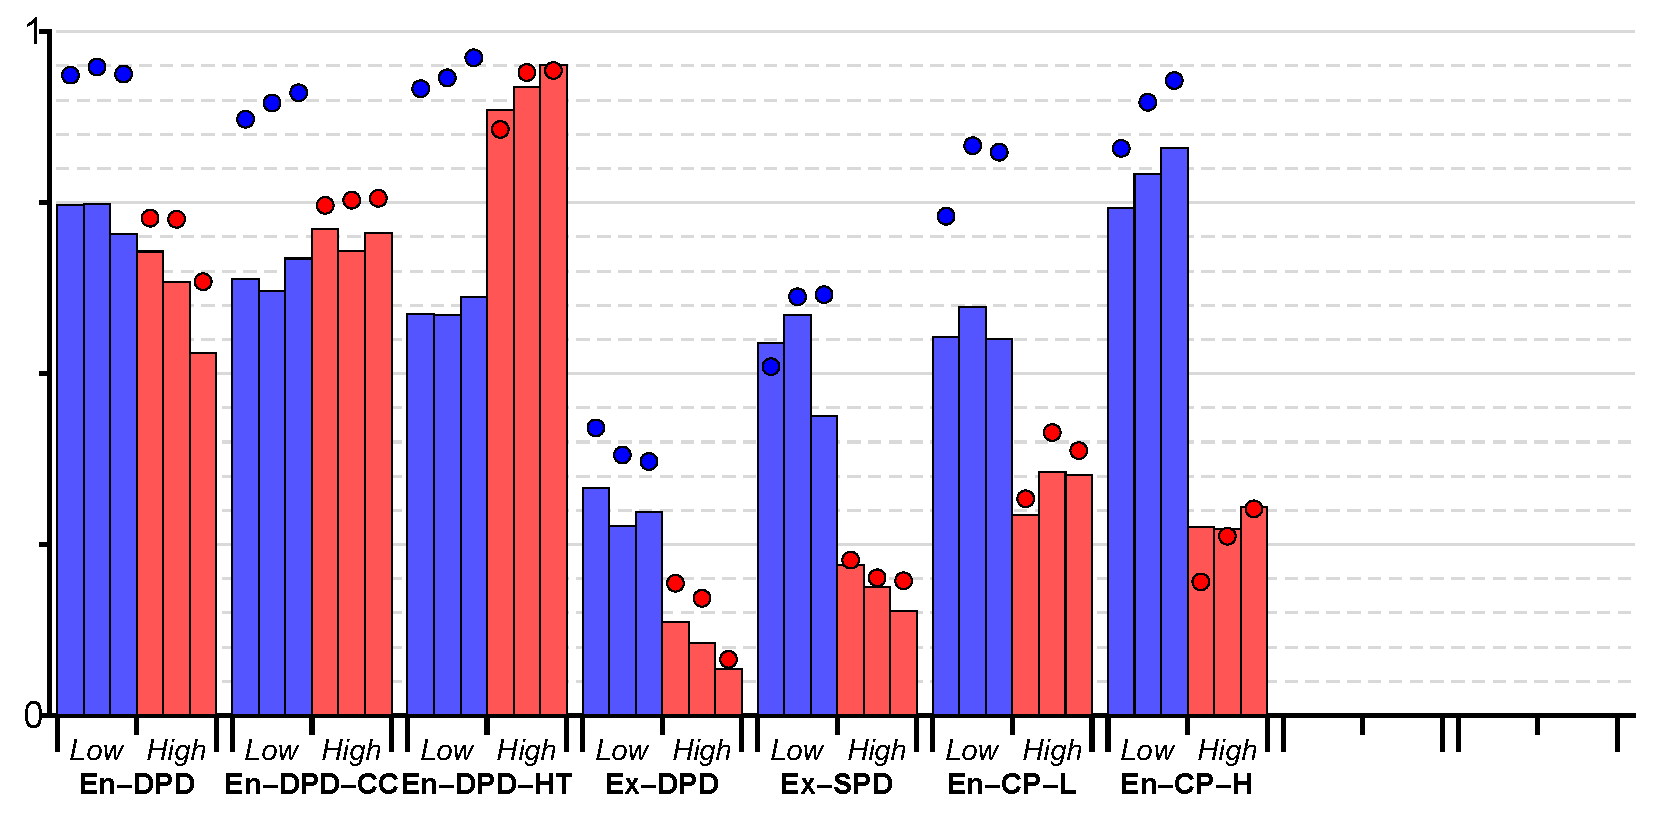
\includegraphics[width=1.0\textwidth]{../../../../p/vw_MPE/img/col_bar_StateCoop_block_CP_H.pdf}
\end{center}

{\small \begin{itemize}\item Points indicate Cooperation rate in first/second round for low/high state
\item Blocks of cycles 1--5, 6--10, 11--15
\end{itemize}
}\end{frame}
\begin{frame}{Subject Cooperation: En-DPD$\rightarrow$\only<2>{En-CP-L}\only<3>{En-CP-H} }


\begin{center}
	\includegraphics<1>[width=0.6\textwidth]{../../../../p/vw_MPE/img/col_subject_stateCooperation_L5_EnDPD_2.pdf}
	\includegraphics<2>[width=0.6\textwidth]{../../../../p/vw_MPE/img/col_subject_stateCooperation_L5_CP_L.pdf}
	\includegraphics<3>[width=0.6\textwidth]{../../../../p/vw_MPE/img/col_subject_stateCooperation_L5_CP_H.pdf}
\end{center}

\end{frame}

\begin{frame}{Sequences: En-CP-L}

\begin{itemize}
\item Five most popular sequences across rounds 1--5 are:

\begin{itemize}
\item \textcolor{red}{CC},\textcolor{blue}{DD},\textcolor{red}{CC},\textcolor{blue}{DD},\textcolor{red}{CC}
(26\% of cycles)
\item \textcolor{red}{CC},\textcolor{blue}{DC},\textcolor{blue}{DD},\textcolor{red}{CC},\textcolor{blue}{DD}
(10\%)
\item \textcolor{red}{CC},\textcolor{blue}{DC},\textcolor{blue}{CD},\textcolor{blue}{DC},\textcolor{blue}{CD}
(10\%)
\item \textcolor{red}{CC},\textcolor{blue}{DD},\textcolor{red}{CC},\textcolor{blue}{DD},\textcolor{red}{DC
}(10\%)
\end{itemize}
\item Mix of MPEs, some D-D, some C-D
\end{itemize}
\end{frame}

\begin{frame}{Sequences: En-CP-H}

\begin{itemize}
\item Five most popular sequences across rounds 1--5 are:

\begin{itemize}
\item \textcolor{red}{CC},\textcolor{blue}{DD},\textcolor{red}{CC},\textcolor{blue}{DD},\textcolor{red}{CC}
(26\% of cycles)
\item \textcolor{red}{CC},\textcolor{blue}{DC},\textcolor{blue}{DD},\textcolor{red}{CC},\textcolor{blue}{DD}
(10\%)
\item \textcolor{red}{CC},\textcolor{blue}{DC},\textcolor{blue}{CD},\textcolor{blue}{DC},\textcolor{blue}{CD}
(10\%)
\item \textcolor{red}{CC},\textcolor{blue}{DD},\textcolor{red}{CC},\textcolor{blue}{DD},\textcolor{red}{DC
}(10\%)
\end{itemize}
\item Looks at or close to MPE
\end{itemize}
\end{frame}


\begin{frame}{Strategies (En-DPD$\rightarrow$En-CP-L$\rightarrow$En-CP-H)}
\begin{itemize}
\item Markov strategies

\begin{itemize}
\item C-C: $7.9\%\rightarrow6.8\%\rightarrow7.8\%$
\item \textbf{C-D:} $23.5\%\rightarrow23.9\%\rightarrow35.4\%$
\item \textbf{D-D:} $4.7\%\rightarrow12.3\%\rightarrow4.8\%$
\end{itemize}
\item Popular history-dependent strategies

\begin{itemize}
\item Grim trigger $11.4\%\rightarrow7.3\%\rightarrow0.0\%$
\item D-Alternate, D-trigger $4.3\%\rightarrow16.1\%\rightarrow4.6\%$
\item C-Alternate, MPE-trigger $23.4\%\rightarrow9.1\%\rightarrow16.1\%$
\item D-Alternate, MPE-trigger $2.5\%\rightarrow17.2\%\rightarrow31.4\%$
\end{itemize}
\item \textbf{More Markov play; Attempts at efficient alternation; Greater
MPE trigger use}
\end{itemize}
\end{frame}
\begin{frame}


\textbf{Result 7: }



\textbf{Removing the static externalities, outcomes look more like
MPE}
\end{frame}


\begin{frame}{Selection Index}
\begin{itemize}
\item In repeated games, a large body of experimental work has shown that
the basin attraction helps predict equilibrium selection
\end{itemize}
{\small{}}%
\begin{tabular}{cc|>{\centering}p{0.18\textwidth}|>{\centering}p{0.18\textwidth}|}
 & \multicolumn{1}{c}{} & \multicolumn{2}{c}{Col:}\tabularnewline
 & \multicolumn{1}{c}{} & \multicolumn{1}{>{\centering}p{0.18\textwidth}}{\textbf{Grim}} & \multicolumn{1}{>{\centering}p{0.18\textwidth}}{\textbf{All-D}}\tabularnewline
\cline{3-4}
\multirow{2}{*}{Row:} & \textbf{Grim} & \textcolor{black}{$1$} & -$S(\delta)$\tabularnewline
\cline{3-4}
 & \textbf{All-D} & $T(\delta)$ & \textcolor{black}{$0$}\tabularnewline
\cline{3-4}
\end{tabular}{\small \par}
\begin{itemize}
\item Scale/Normalized so (D,D)=0, (C,C)=1
\item $S(\delta)=(1-\delta)\cdot s$ and $T(\delta)=(1-\delta)(1+t)$
\item Basin of attraction is $p=\tfrac{S(\delta)}{1+S(\delta)-T(\delta)}$
\end{itemize}
\end{frame}

\begin{frame}{Selection Index}

{\small{}}%
\begin{tabular}{cc|>{\centering}p{0.18\textwidth}|>{\centering}p{0.18\textwidth}|}
 & \multicolumn{1}{c}{} & \multicolumn{2}{c}{Col:}\tabularnewline
 & \multicolumn{1}{c}{} & \multicolumn{1}{>{\centering}p{0.18\textwidth}}{\textbf{Grim}} & \multicolumn{1}{>{\centering}p{0.18\textwidth}}{\textbf{All-D}}\tabularnewline
\cline{3-4}
\multirow{2}{*}{Row:} & \textbf{Grim} & \textcolor{black}{$1$} & -$S(\delta)$\tabularnewline
\cline{3-4}
 & \textbf{All-D} & $T(\delta)$ & \textcolor{black}{$0$}\tabularnewline
\cline{3-4}
\end{tabular}{\small \par}
\begin{itemize}
\item Looks at a cooperative strategy, and the MPE, where miscoordination
reverts to individual rationality
\item We try to mirror this in a dynamic game
\end{itemize}
\end{frame}

\begin{frame}{Selection Index}

{\small{}}%
\begin{tabular}{cc|>{\centering}p{0.18\textwidth}|>{\centering}p{0.18\textwidth}|}
 & \multicolumn{1}{c}{} & \multicolumn{2}{c}{Col}\tabularnewline
 & \multicolumn{1}{c}{} & \multicolumn{1}{>{\centering}p{0.18\textwidth}}{\textbf{Strategy 1}} & \multicolumn{1}{>{\centering}p{0.18\textwidth}}{\textbf{Strategy 2}}\tabularnewline
\cline{3-4}
\multirow{2}{*}{Row:} & \textbf{Strategy 1} & $U(s_{1},s_{1},\omega)$ & $S(\delta,\omega)$\tabularnewline
\cline{3-4}
 & \textbf{Strategy 2} & $T(\delta,\omega)$ & $U(s_{2},s_{2},\omega)$\tabularnewline
\cline{3-4}
\end{tabular}{\small \par}
\begin{itemize}
\item We calculate the basin of attraction by state $p(\omega)$

\begin{itemize}
\item Riskiness of coordination really depends on the particular state
\end{itemize}
\item Calculate $S(\delta,\omega)$ and $T(\delta,\omega)$ using the worst-case
outcome on miscoordination

\begin{itemize}
\item the IR payoff from the point that strategies $s_{1}$ and $s_{2}$
identifiably diverge
\item Calculations include the dynamics and identification components
\end{itemize}
\end{itemize}
\end{frame}
\begin{frame}{Summary}

\begin{itemize}
\item Manipulation results:

\begin{itemize}
\item Subjects target efficiency, even if asymmetric
\item Readily internalize own effect on dynamics
\item A more complex but strategically similar game has similar behavior
\item Without endogenous dynamics, cooperation collapses
\item A changing environment makes cooperation slightly harder
\item Removing static externalities leads to more MPE behavior
\end{itemize}
\end{itemize}
\end{frame}

\begin{frame}{Salz \& Vespa (2014) }
	\begin{itemize}
		\item Markov Perfection is commonly used in the IO literature as an equilibrium solution concept to identify parameters\pause
		\item For example, in oligopolistic competition with entry/exit:
		\begin{itemize}
			\item Under Markov, the equilibrium can be characterized given the structural parameters as $\Psi(\beta)$
			\item Given data on the entry/exit decisions of firms we can use $\Psi^{-1}(\cdot)$ to help tell us about the likely parameters $\beta$
		\end{itemize}\pause
		\item But our conclusions may be very sensitive to whether or not Markov was actually the selected equilibrium!
	\end{itemize}
\end{frame}

\begin{frame}{Salz \& Vespa (2014) }
	\begin{itemize}
		\item Examine a repeated PD game (framed in the paper as a Cournot game) with entry/exit \pause
		\begin{itemize}
			\item In each round those in the market face can make $\phi_it$ by exiting the marker, where $\phi_{it}\sim\mathcal{U}[0,100]$
			\item Those outside of the market face an entry cost $\tau+\psi_it$, where $\psi_{it}\sim\mathcal{U}[0,100]$
		\end{itemize}\pause
		\item State variable $\omega$ here is the entry/exit status of the two players, and the current scrap/entry draw.
		\item Markov has each participant play the Cournot quantity when in the market and use a cutoff rule for entry and exit decisions
	\end{itemize}
\end{frame}


\begin{frame}{Salz \& Vespa (2014) }
\begin{center}
	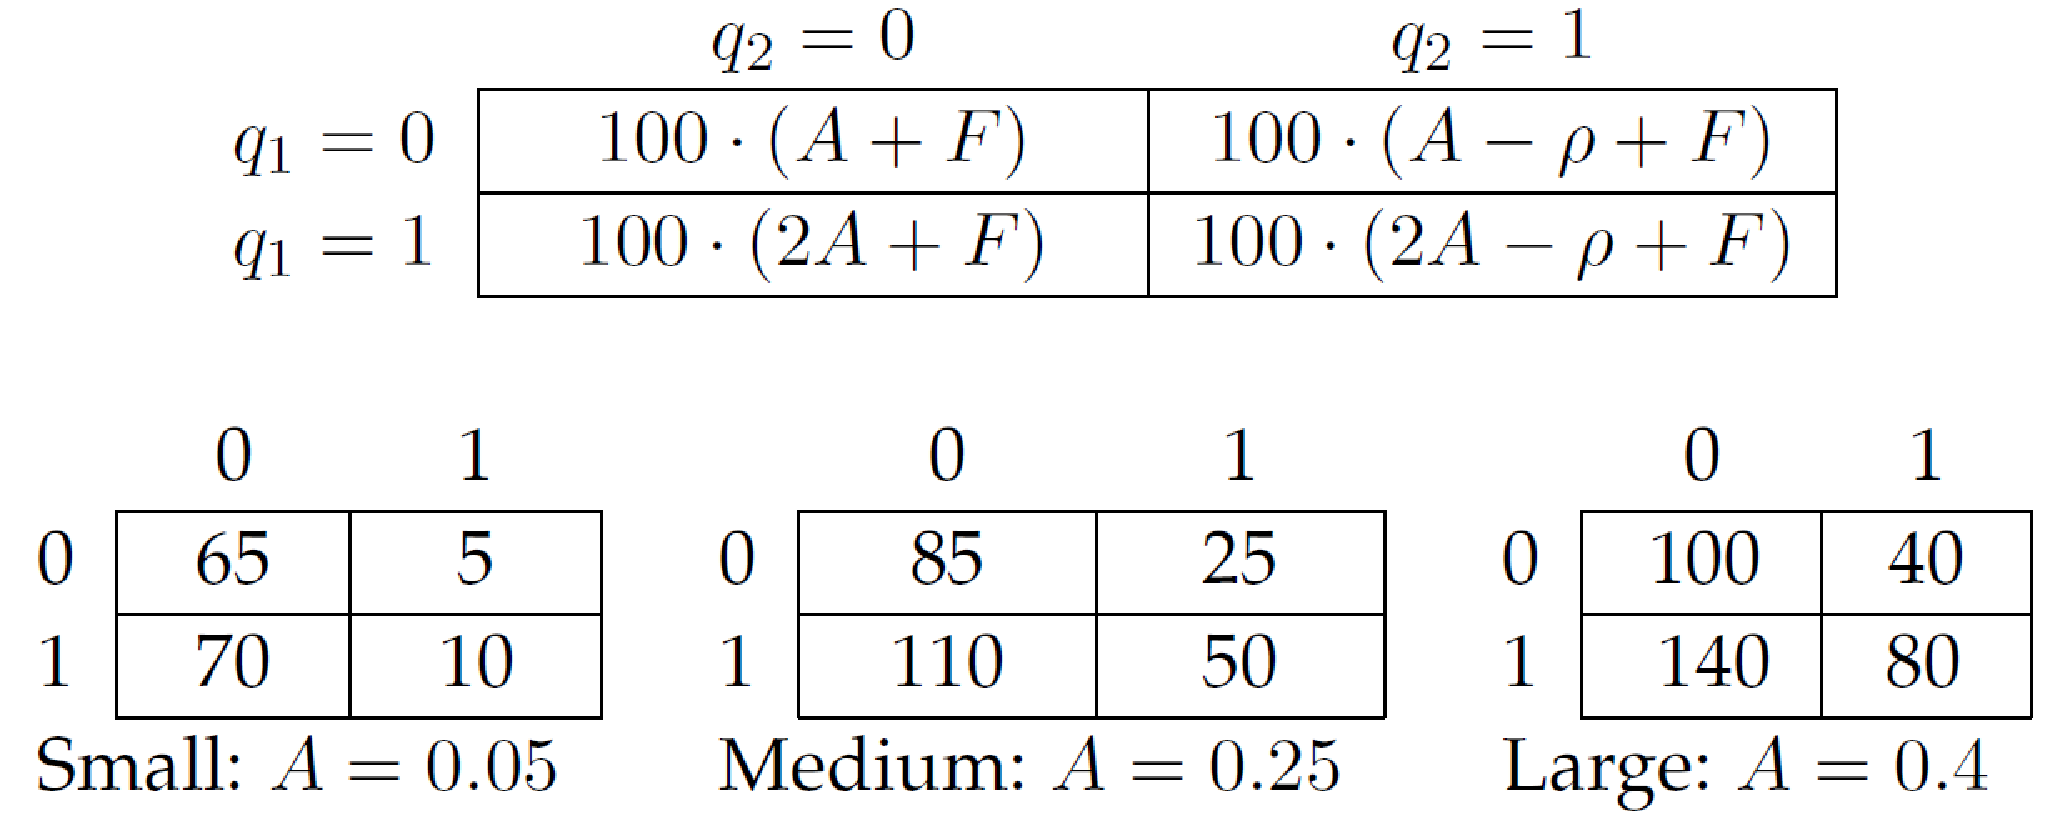
\includegraphics[width=0.8\textwidth]{../img/SVtbl1.pdf}
\end{center}
	\begin{itemize}
		\item Vary the size of the pie (the $A$ parameter in a cournot game)
		\item Exit values are worth between 0 and 100
		\item Entry costs are between 15 and 115\pause
		\item But there are also collusive SPE if both play monopoly quantity!
	\end{itemize}
\end{frame}


\begin{frame}{Salz \& Vespa (2014) }
\begin{center}
	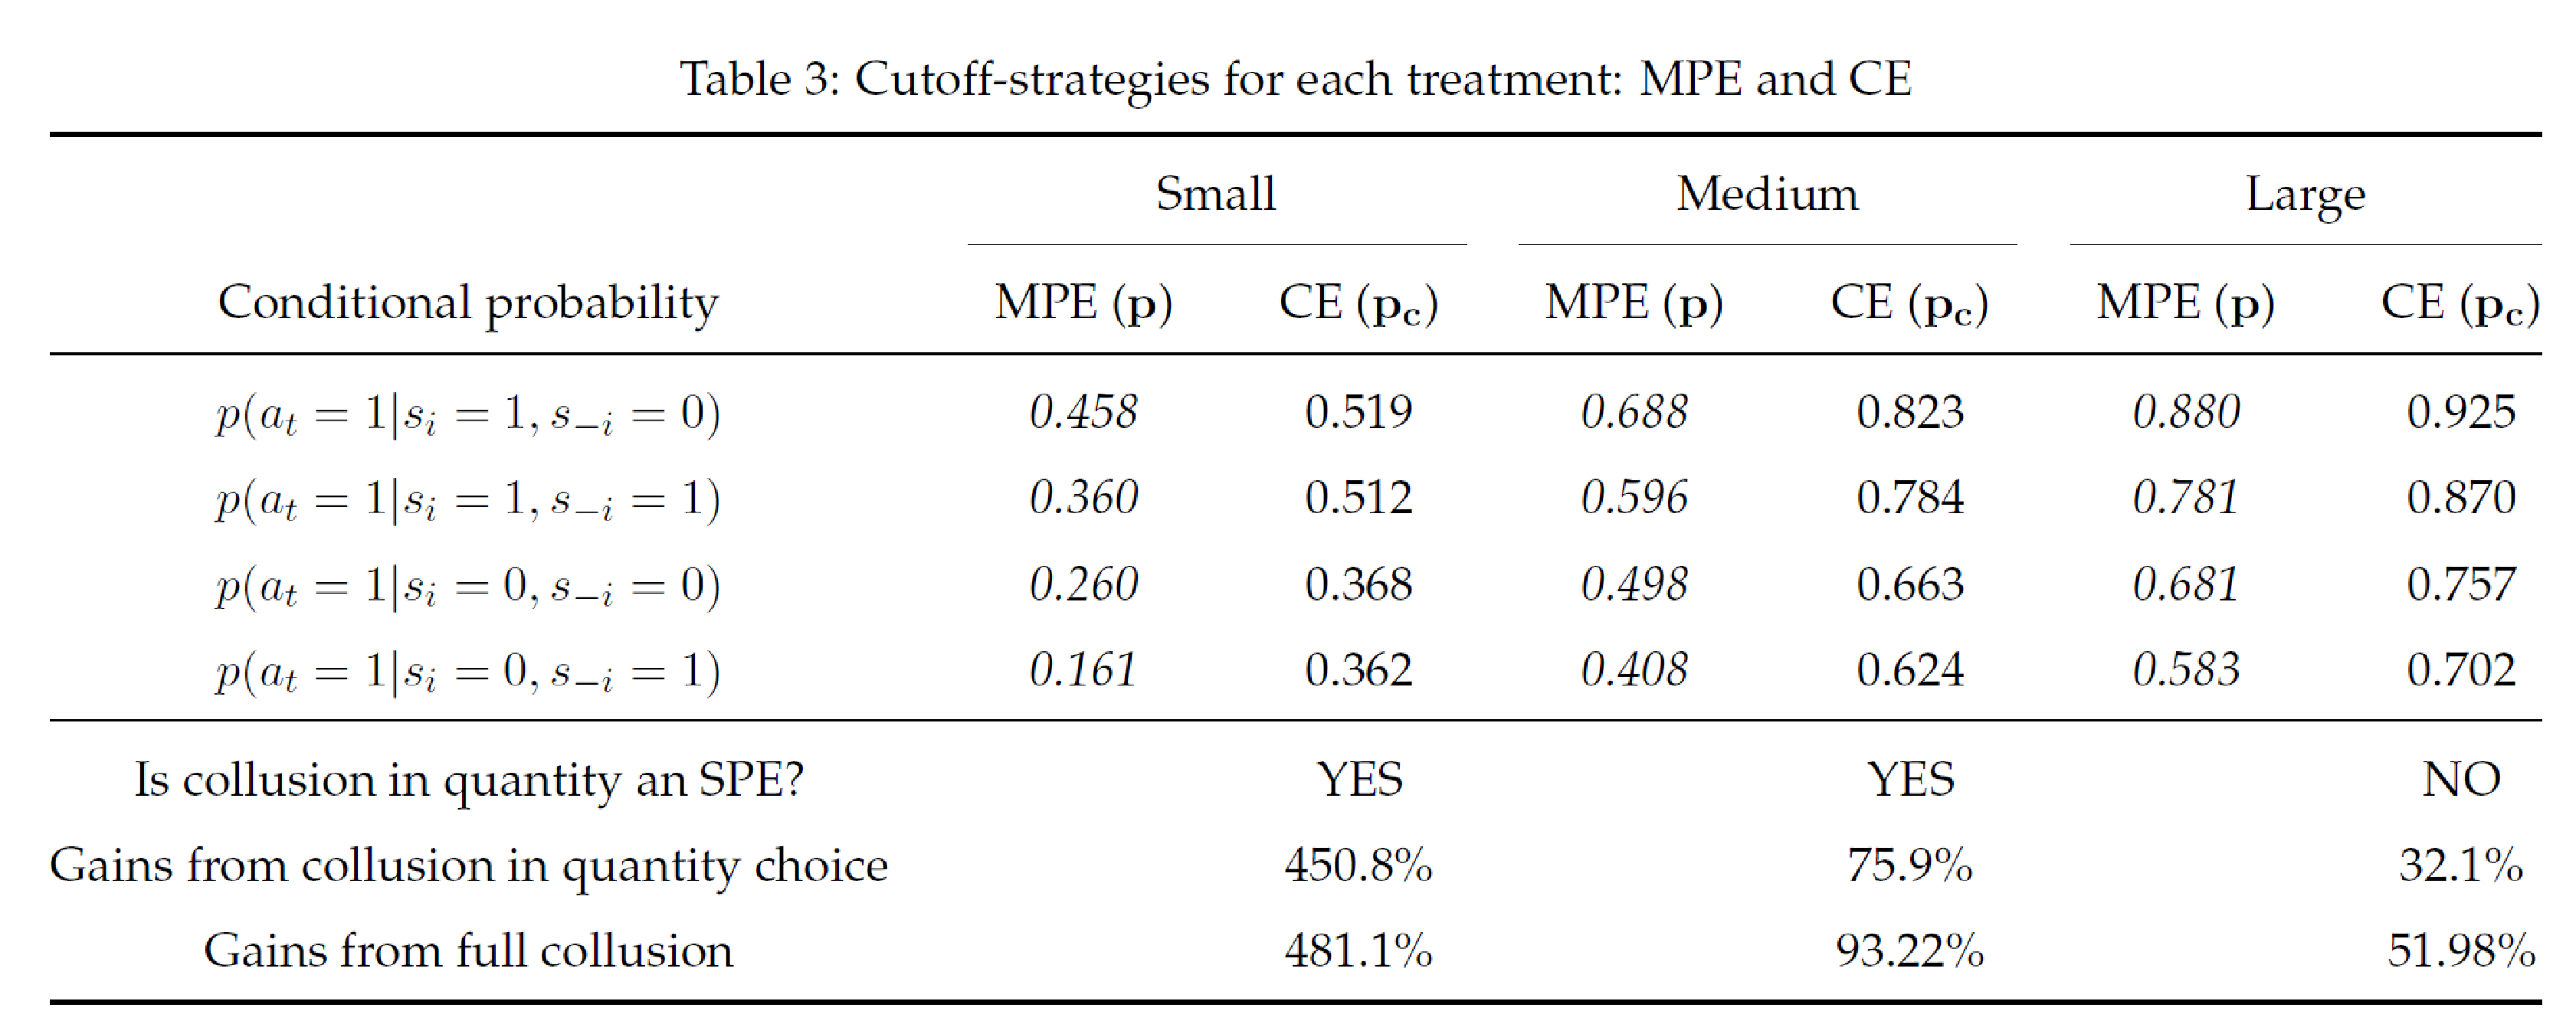
\includegraphics[width=0.8\textwidth]{../img/SVtbl2.pdf}
\end{center}
	\begin{itemize}
		\item Probability of entry depends on who is presently in game
		\item Paper will attempt to remove CE by forcing the Cournot quantity in the stage game
	\end{itemize}
\end{frame}


\begin{frame}{Salz \& Vespa (2014) }
\begin{center}
	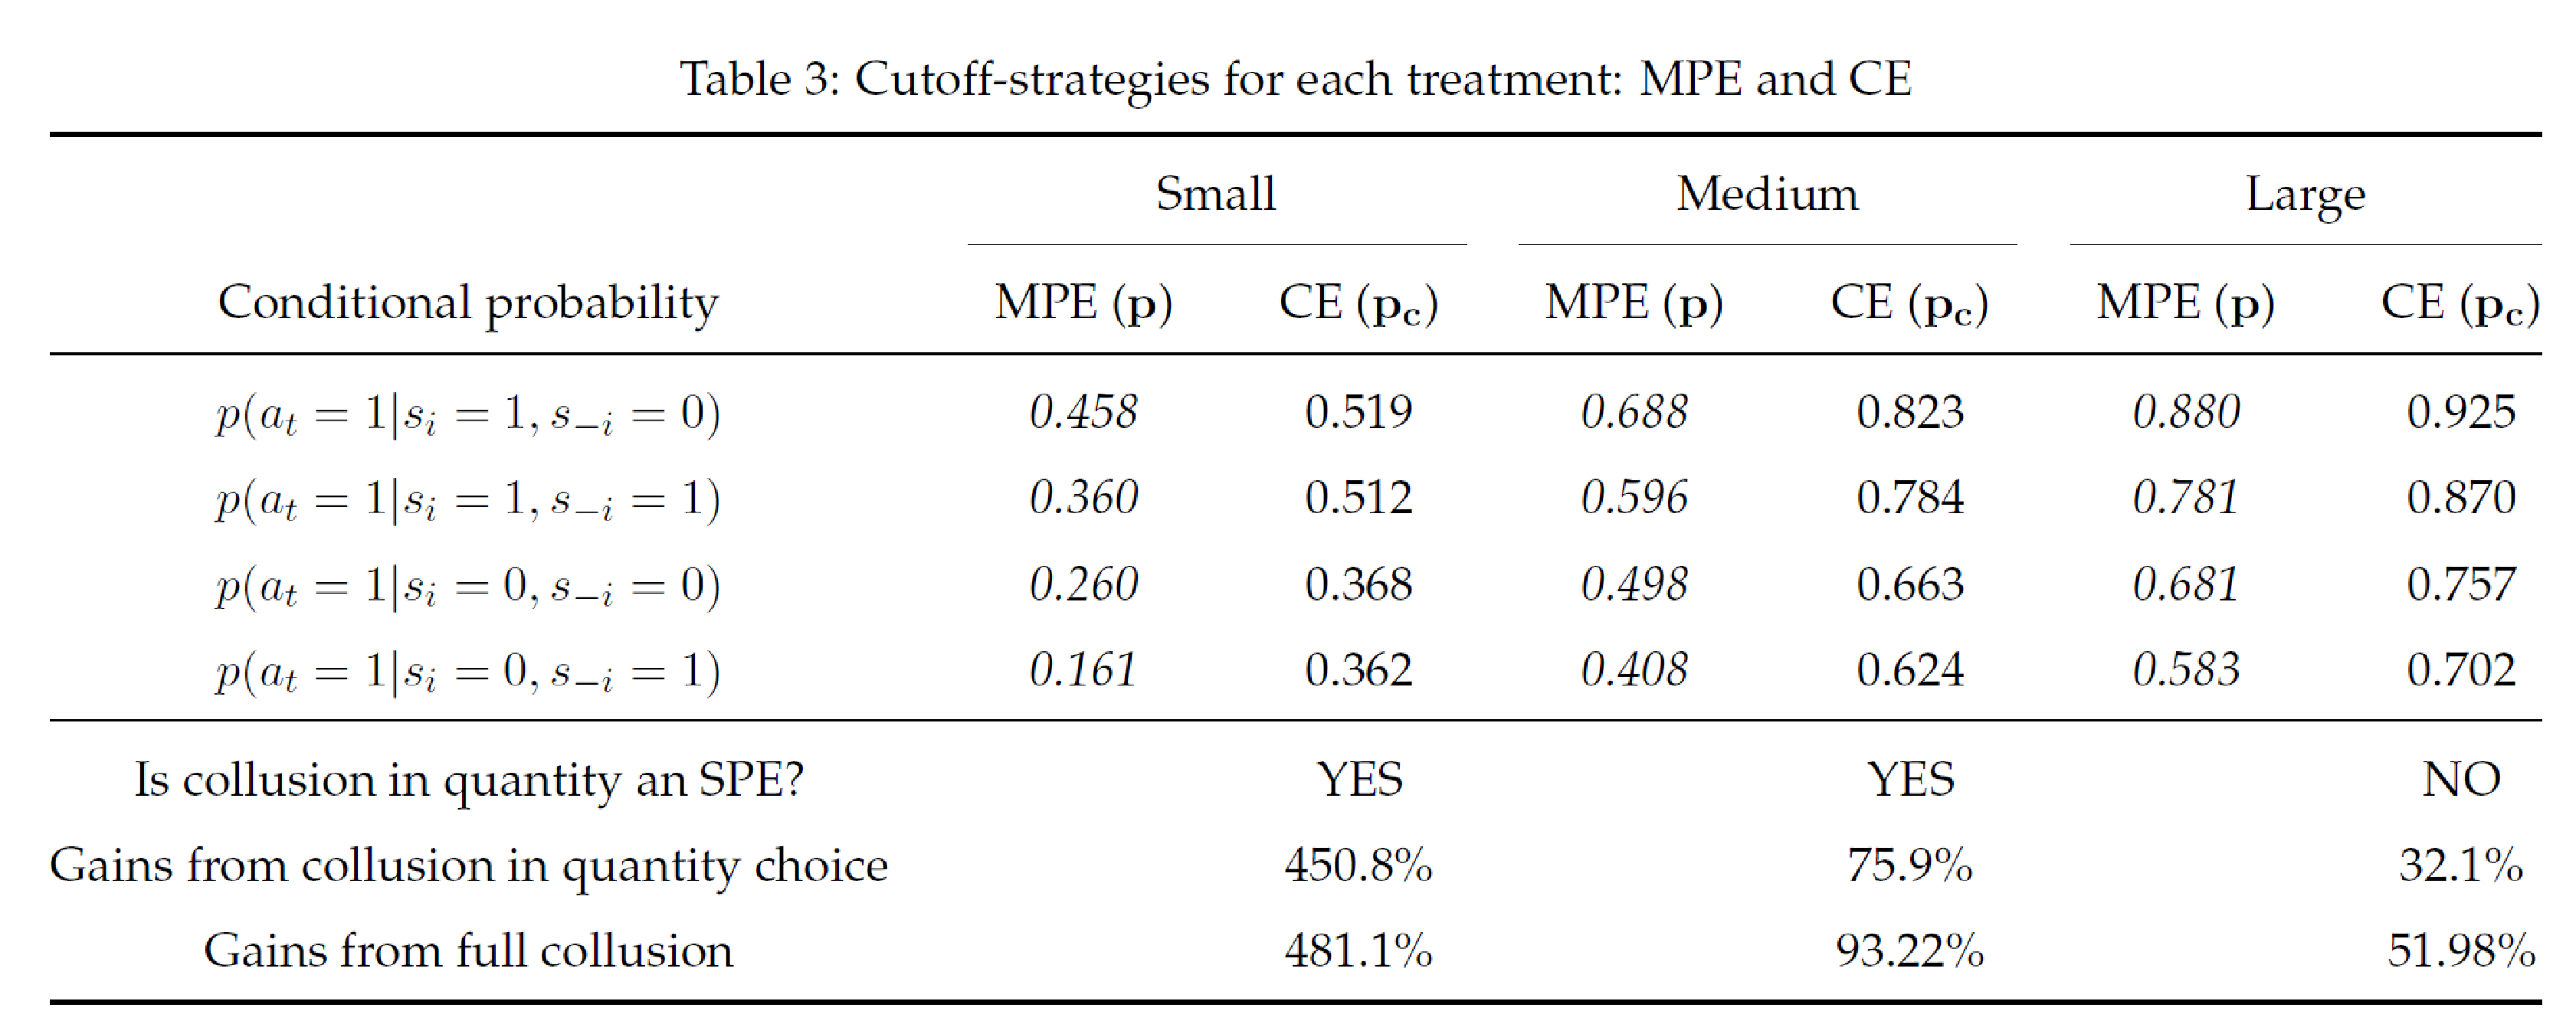
\includegraphics[width=0.8\textwidth]{../img/SVtbl2.pdf}
\end{center}
	\begin{itemize}
		\item Probability of entry depends on who is presently in game
		\item Paper will attempt to remove CE by forcing the Cournot quantity in the stage game
	\end{itemize}
\end{frame}

\begin{frame}{Salz \& Vespa (2014) }
	\begin{itemize}
		\item UC Santa Barabara subjects
		\item Three sessions per treatment
		\item Three values for $A$
		\item Either PD game or force Cournot Quantity
		\item Average earnings of \$19
		\item Continuation probability is $\delta=\tfrac{4}{5}$
		\item Block design
	\end{itemize}
\end{frame}

\begin{frame}{Salz \& Vespa (2014) }
	\begin{center}
		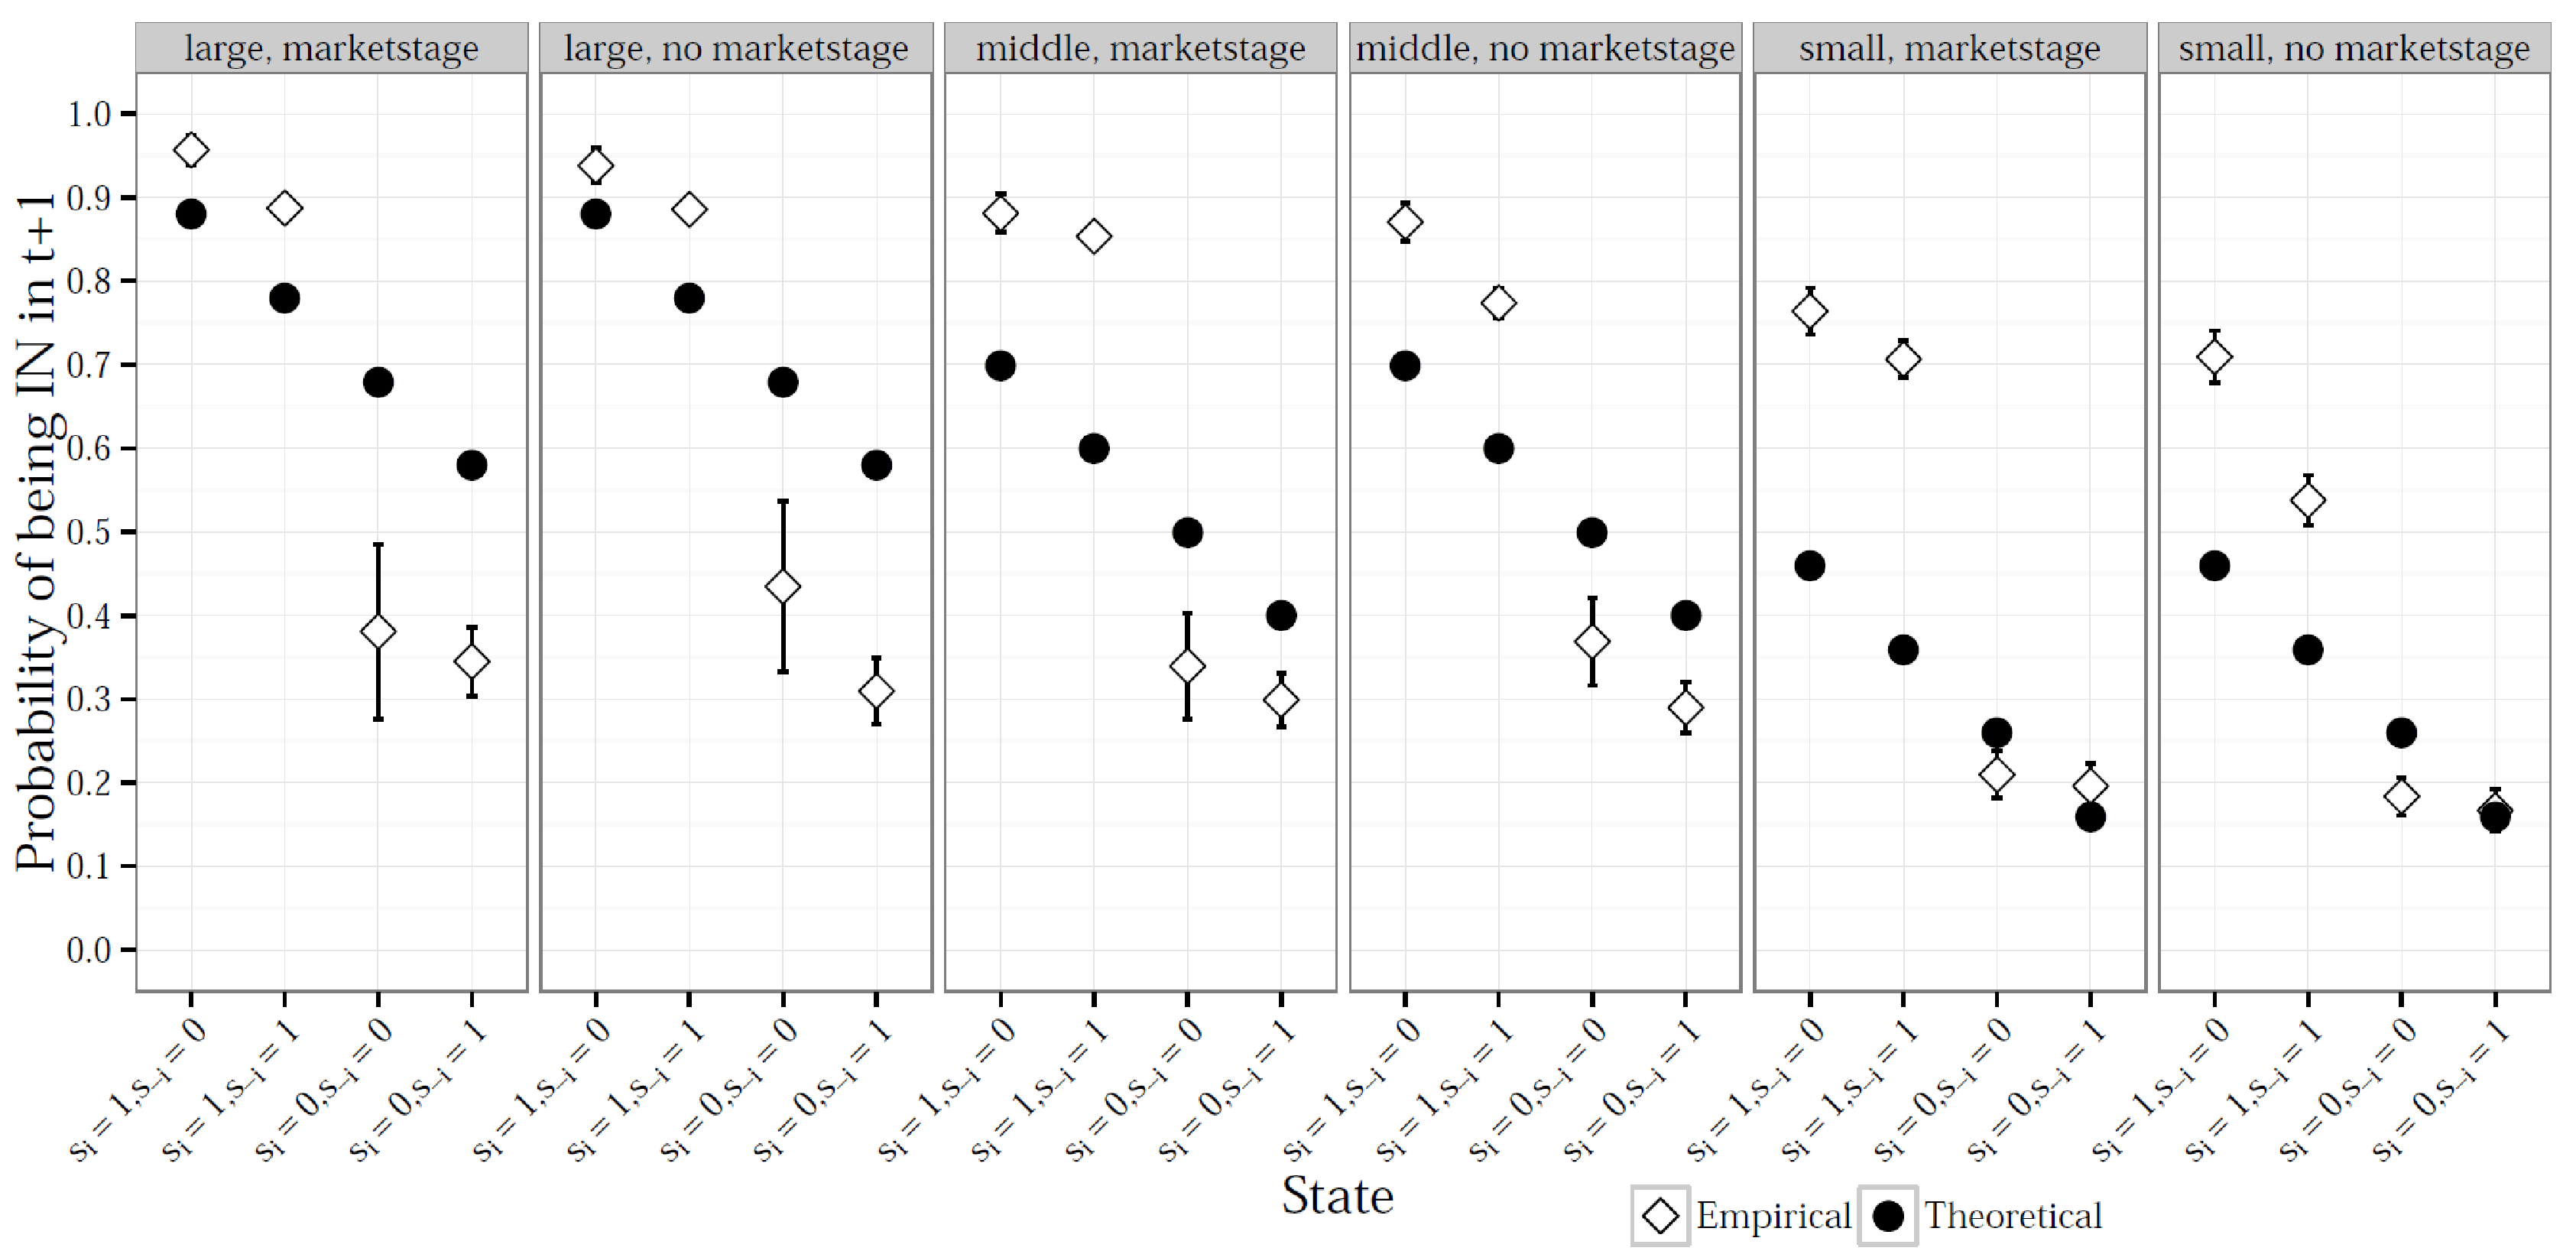
\includegraphics[width=0.8\textwidth]{../img/SVfig2.pdf}
	\end{center}

	\begin{itemize}
		\item Greater inertia than predicted by MPE
		\item Stay out more if already out
		\item Stay in more if already in
	\end{itemize}

\end{frame}

\begin{frame}{Salz \& Vespa (2014) }
	\begin{center}
		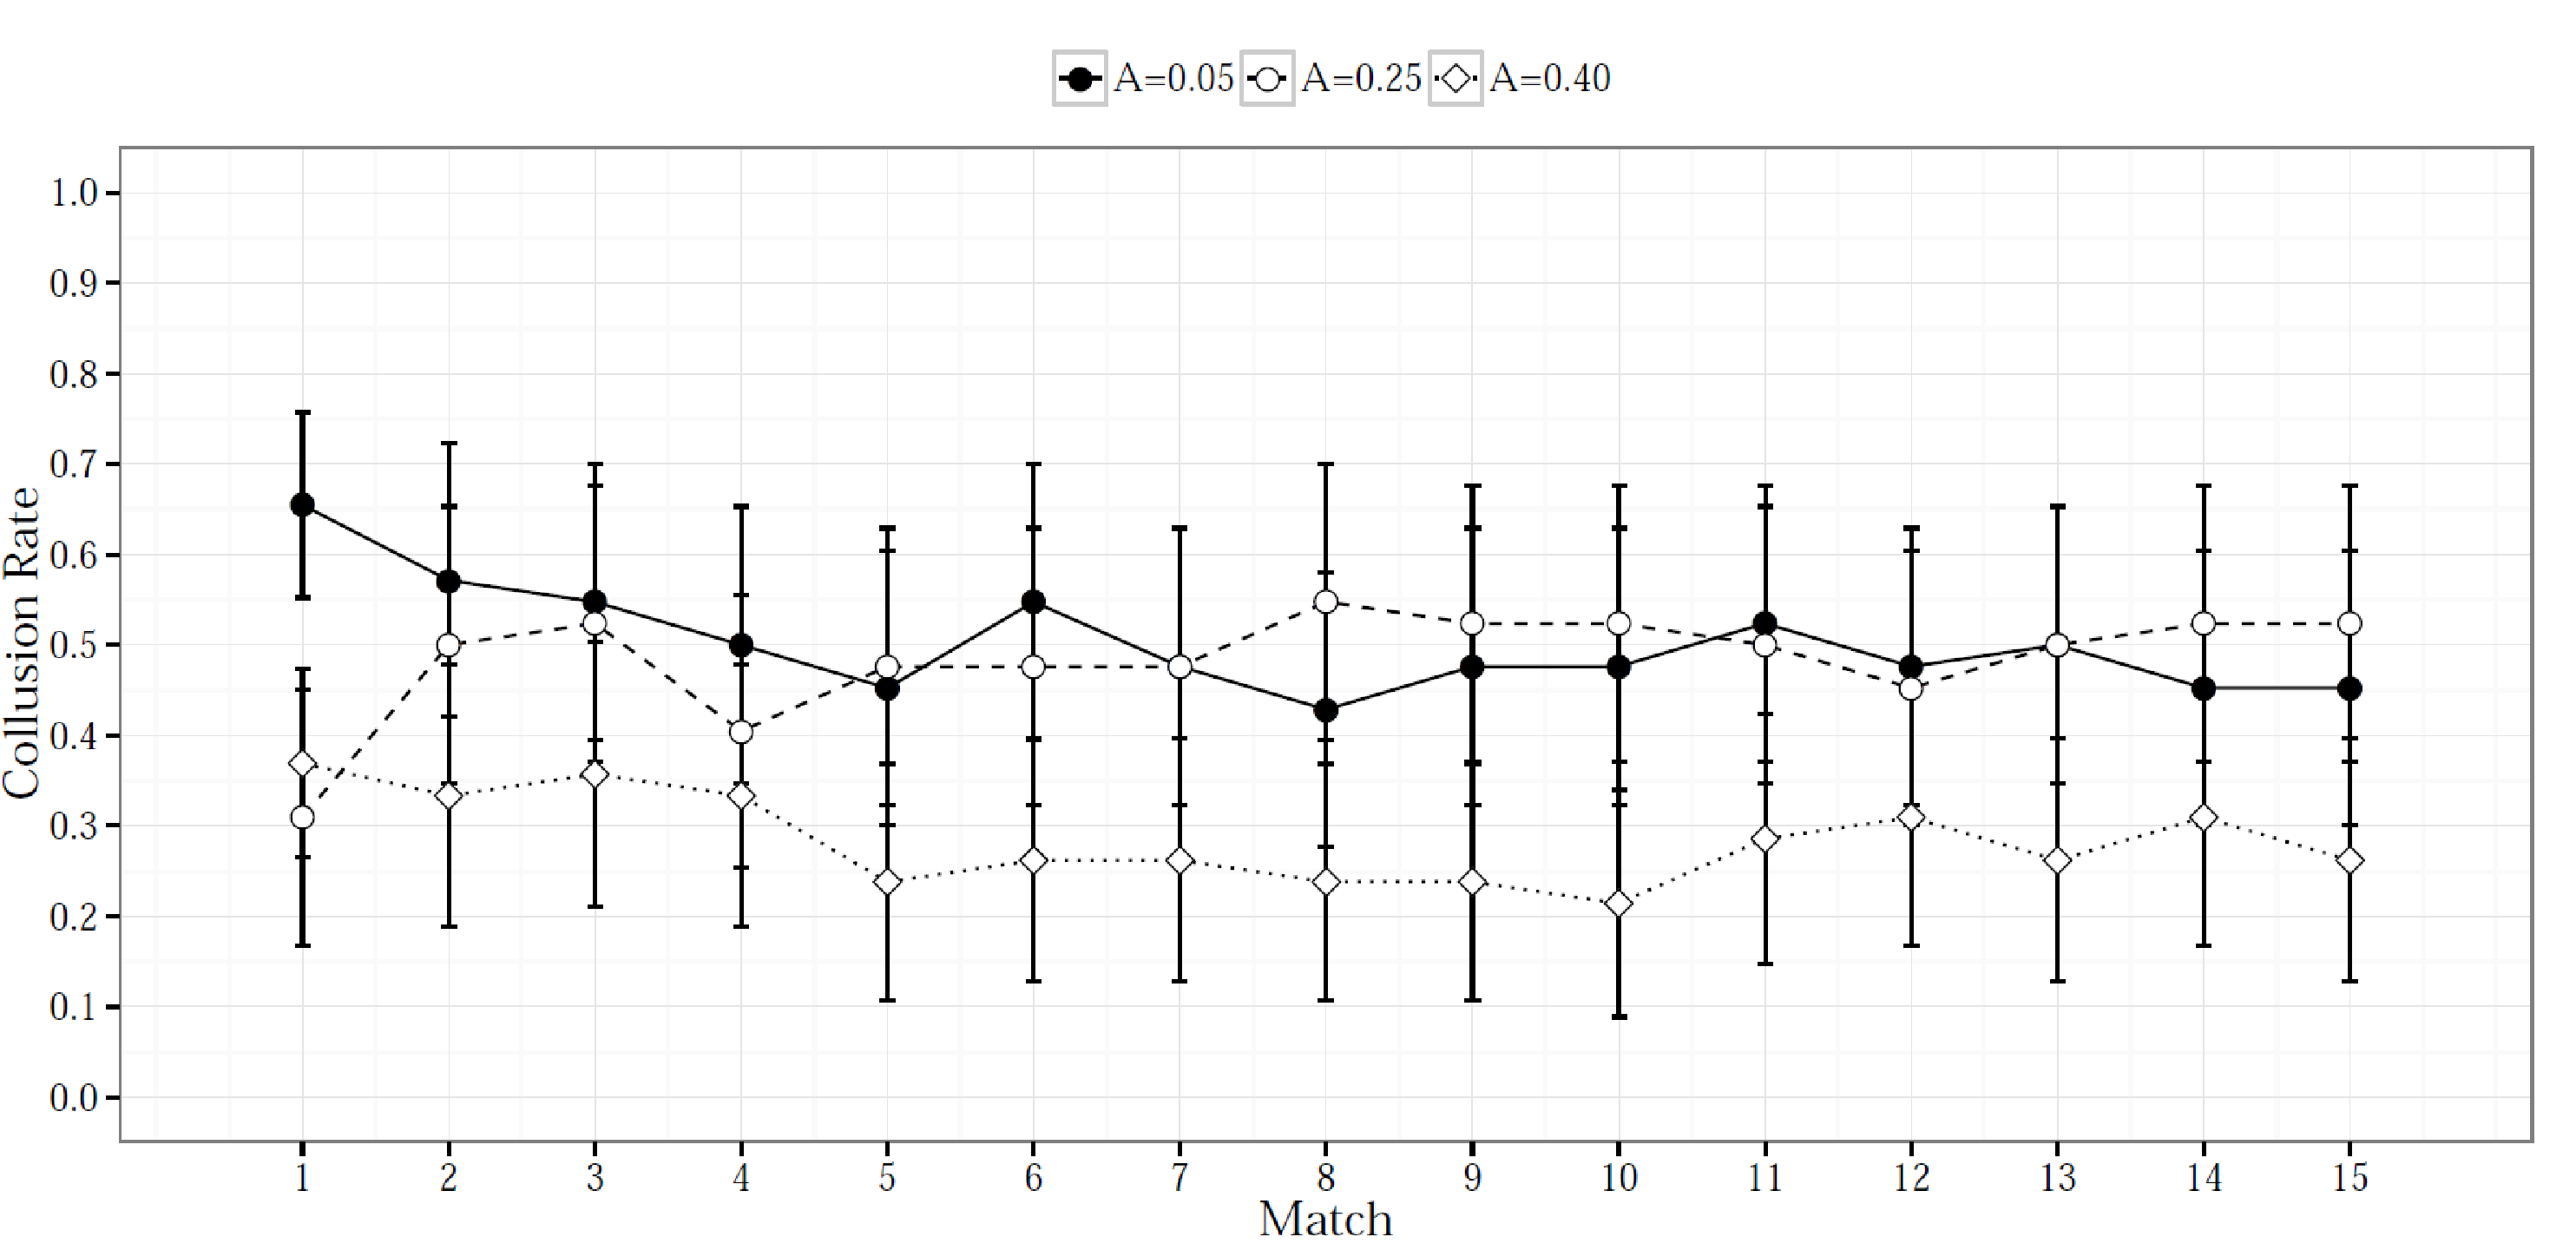
\includegraphics[width=0.8\textwidth]{../img/SVfig3.pdf}
	\end{center}

	\begin{itemize}
		\item Greater collusion in markets with lower $A$
		\item Matches reapeated game results as cooperation is less risky
	\end{itemize}

\end{frame}

\begin{frame}{Salz \& Vespa (2014) }
	\begin{itemize}
		\item Use Bajari, Benkard and Levin (EMA 2007) to estimate parameters of the game
		\item Using the observed probabilities of entry/exit, the estimation procedure spits out the
		\begin{item}
		\item Implied market size $A$
		\item Competitive effect $\rho$
		\item The fixed entry costs $\tau$
		\end{itemize}\pause
		\item Discount $\delta$ and the distribution of scrap/entry costs are assumed to be known by econometrician
	\end{itemize}
\end{frame}


\begin{frame}{Salz \& Vespa (2014) }

\begin{center}
		\includegraphics<1>[width=0.8\textwidth]{../img/SVtbl5-1.pdf}
		\includegraphics<2>[width=0.8\textwidth]{../img/SVtbl5-2.pdf}
		\includegraphics<3>[width=0.8\textwidth]{../img/SVtbl5-3.pdf}
	\end{center}
	\begin{itemize}
		\item Parameters assessed using the experimental data
		\begin{itemize}
			\item True parameters are $\tau$ is 0.15, and $\rho$ is 0.6
		\end{itemize}
	\end{itemize}
\end{frame}

\begin{frame}{Salz \& Vespa (2014) }

	\begin{itemize}
		\item Using the estimated parameters, they then examine counterfactuals\pause
		\item For example:
		\begin{itemize}
			\item The large markets has $A=0.4$, medium $A=0.25$
			\item Rescale the estimated large market by $\tfrac{0.25}{0.40}$
			\item Does the implied behavior look like the medium market?
		\end{itemize}
	\end{itemize}
\end{frame}

\begin{frame}{Salz \& Vespa (2014) }
\begin{center}
		\includegraphics<1>[width=0.8\textwidth]{../img/SVtbl6.pdf}
	\end{center}
	\begin{itemize}
		\item Look at mean average error for prediction $p$
		\item Mean average valuation error over continuations
		\item $R$ is the ratio of this error to the maximum possible under full collusion
	\end{itemize}
\end{frame}

\begin{frame}{Salz \& Vespa (2014) }
	The majority of the differences are shown to come from inertia in the decisions, rather than selection of equilibria
\end{frame}

\begin{frame}{Wilson \& Wu (2014) }
	Simpler state space Exit decisions
\end{frame}



\end{document}
